\documentclass[hyperref={pdfpagelabels=false},aspectratio=34,14pt]{beamer}
\usepackage{lmodern} %TODO: descobrir o que mudou as fontes dos slides (comparar com os primeiros)
\usepackage[utf8]{inputenc}
\usepackage[T1]{fontenc}
\usefonttheme[onlymath]{serif}
\usepackage[brazil]{babel}
\usepackage[outputdir=..]{minted}
\usepackage{xcolor}
\usepackage{soul} % strikethrough
\usepackage{advdate}
\usepackage{graphicx}
\usepackage[ampersand]{easylist}
\usepackage{multirow}
\usepackage{tikz}
\usetikzlibrary{shapes,arrows,positioning}
\usetikzlibrary{circuits.logic.US}
\usetikzlibrary{matrix,calc}
\usepackage{karnaugh-map}

\usepackage{pgfpages}
\setbeamertemplate{note page}{\pagecolor{yellow!5}\insertnote}\usepackage{palatino}
\newcommand{\yes}{edge node [above] {yes}}
\newcommand{\no}{edge  node [left]  {no}}
\newcommand{\textttb}[1]{\textcolor{blue}{\ttfamily #1}}

% \setmathfont{Latin Modern Math}[version=lm]

\graphicspath{{../figs/}}

\definecolor{bgc}{rgb}{0.95,0.9,0.95}
\definecolor{links}{HTML}{2A7F7F}
\hypersetup{colorlinks,linkcolor=,urlcolor=links}

\newminted{verilog}{fontsize=\scriptsize, 
		   linenos,
		   numbersep=8pt,
           bgcolor=bgc,
           tabsize=4,
		   framesep=3mm} 
%		   frame=lines,

\newcommand{\verilog}[1]{\verilogf{#1}{\footnotesize}

\newcommand{\verilogf}[2]{\inputminted[fontsize=#2, 
		   linenos,
		   tabsize=2,
		   numbersep=4pt,
           bgcolor=bgc,
		   framesep=3mm]{verilog}{../codes/#1.v}
}

\newminted{nasm}{fontsize=\scriptsize, 
		   linenos,
		   numbersep=8pt,
           bgcolor=bgc,
		   framesep=3mm} 

% \author[shortname]{\scriptsize Prof. Edilson Kato \and Prof. Maurício Figueiredo \and Prof. Ricardo Menotti\newline
% \href{mailto:kato@ufscar.br}{kato@ufscar.br} \and    \href{mailto:mauricio@ufscar.br}{mauricio@ufscar.br} \and
% \href{mailto:menotti@ufscar.br}{menotti@ufscar.br}}

\newcommand{\newauthor}[2]{
  \parbox{0.40\textwidth}{
    \texorpdfstring
      {
        \centering
        \footnotesize #1 \newline
        {\scriptsize{\urlstyle{same}\href{mailto:#2}{#2}\urlstyle{tt}}}
      }
      {#1} \newline
  }
}

\author{
%   \newauthor{Prof. Edilson Kato}{kato@ufscar.br}
% \and
  \newauthor{Prof. Ricardo Menotti}{menotti@ufscar.br}
\and 
  \newauthor{Prof. Maurício Figueiredo}{mauricio@ufscar.br}
% \and
%   \newauthor{Prof. Roberto Inoue}{rsinoue@ufscar.br}
}

\institute{\href{http://www.dc.ufscar.br/}{Departamento de Computação} \\
           \href{http://www.ufscar.br/}{Universidade Federal de São Carlos}} 
\titlegraphic{
  \makebox[.85\paperwidth]{
    
\includegraphics[height=1cm]{figs/LogoDC} 
    \hfill 
    
\includegraphics[height=1cm]{figs/LogoUfscar}}}
\date{Atualizado em: \today} 
% \date{\DayAfter[+1]} % +/-

%\logo{
\includegraphics[height=1cm]{figs/LogoUfscar}
\includegraphics[height=1cm]{figs/LogoDC}}

\title{Lógica Digital (1001351)}

\AtBeginSubsection[]
{
  \begin{frame}<beamer>{Roteiro}
    \tableofcontents[currentsection,currentsubsection]
  \end{frame}
}

\addtobeamertemplate{navigation symbols}{}{%
    \usebeamerfont{footline}%
    \usebeamercolor[fg]{footline}%
    \hspace{1em}%
    \raisebox{1.2pt}[0pt][0pt]{\insertframenumber/\inserttotalframenumber}
}


\title{Implementação de Sistemas Digitais em Verilog}

\subtitle{Laboratório de Arquitetura e Organização de Computadores I} % prática

\begin{document}

\begin{frame}
	\titlepage
\end{frame} 

\begin{frame}{Roteiro}
  \tableofcontents
  % You might wish to add the option [pausesections]
\end{frame}

% Section and subsections will appear in the presentation overview
% and table of contents.

\section{Sistemas de Numeração}

\subsection{Conceitos} 

\frame{
    \frametitle{Bases}
    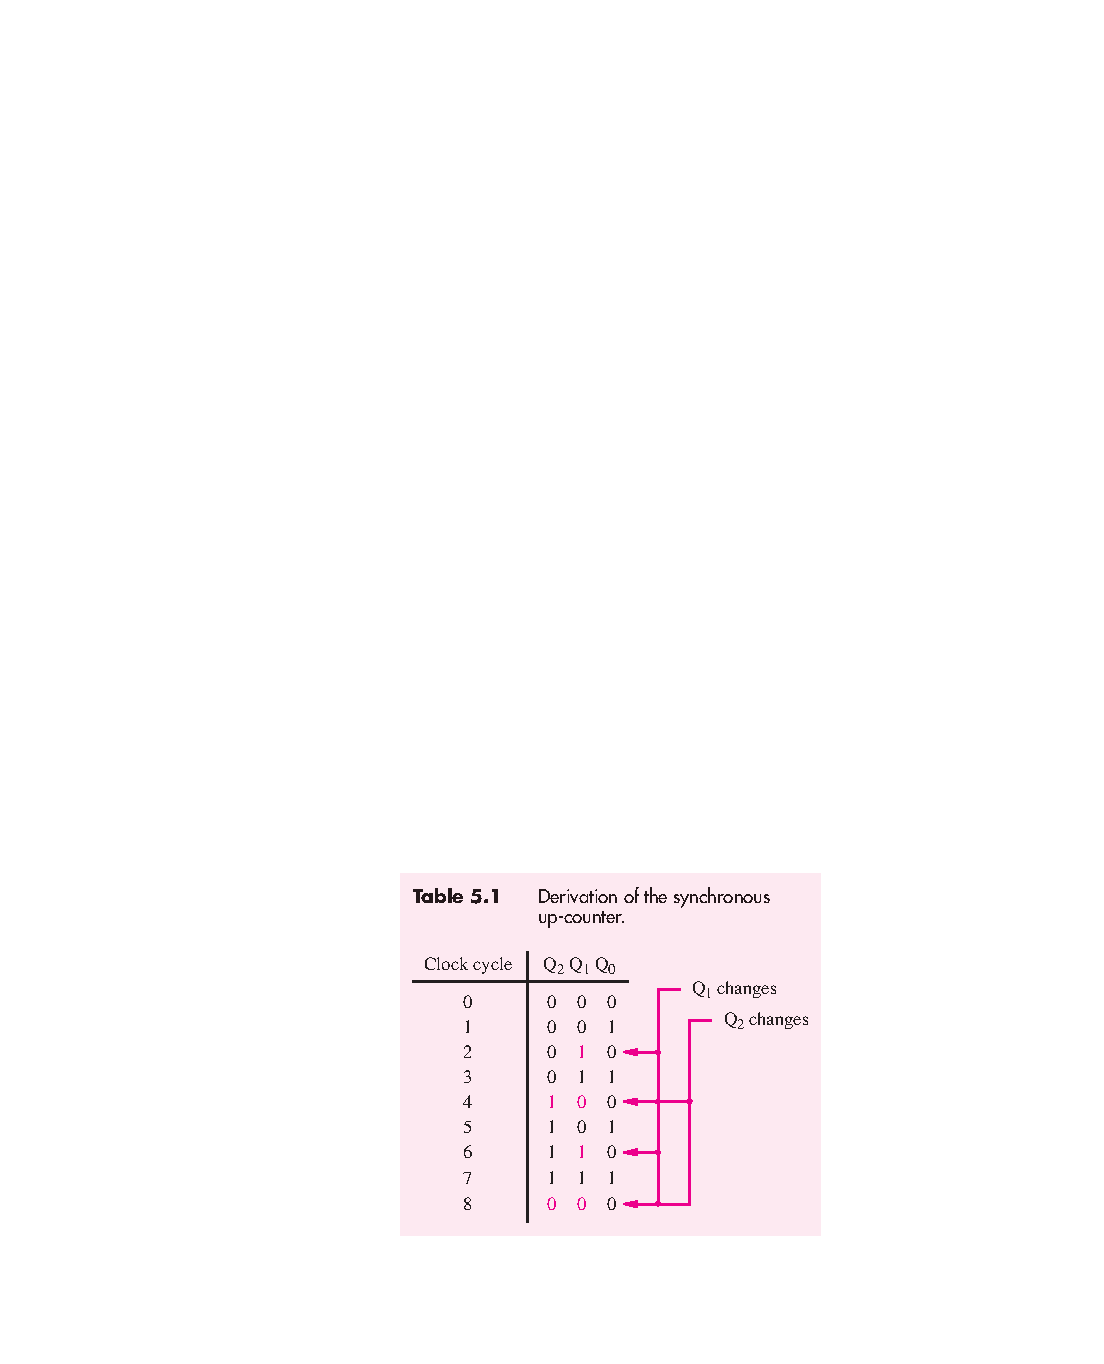
\includegraphics[scale=.7]{figs/VerilogTab5_1}
}

\frame{
    \frametitle{Adição}
    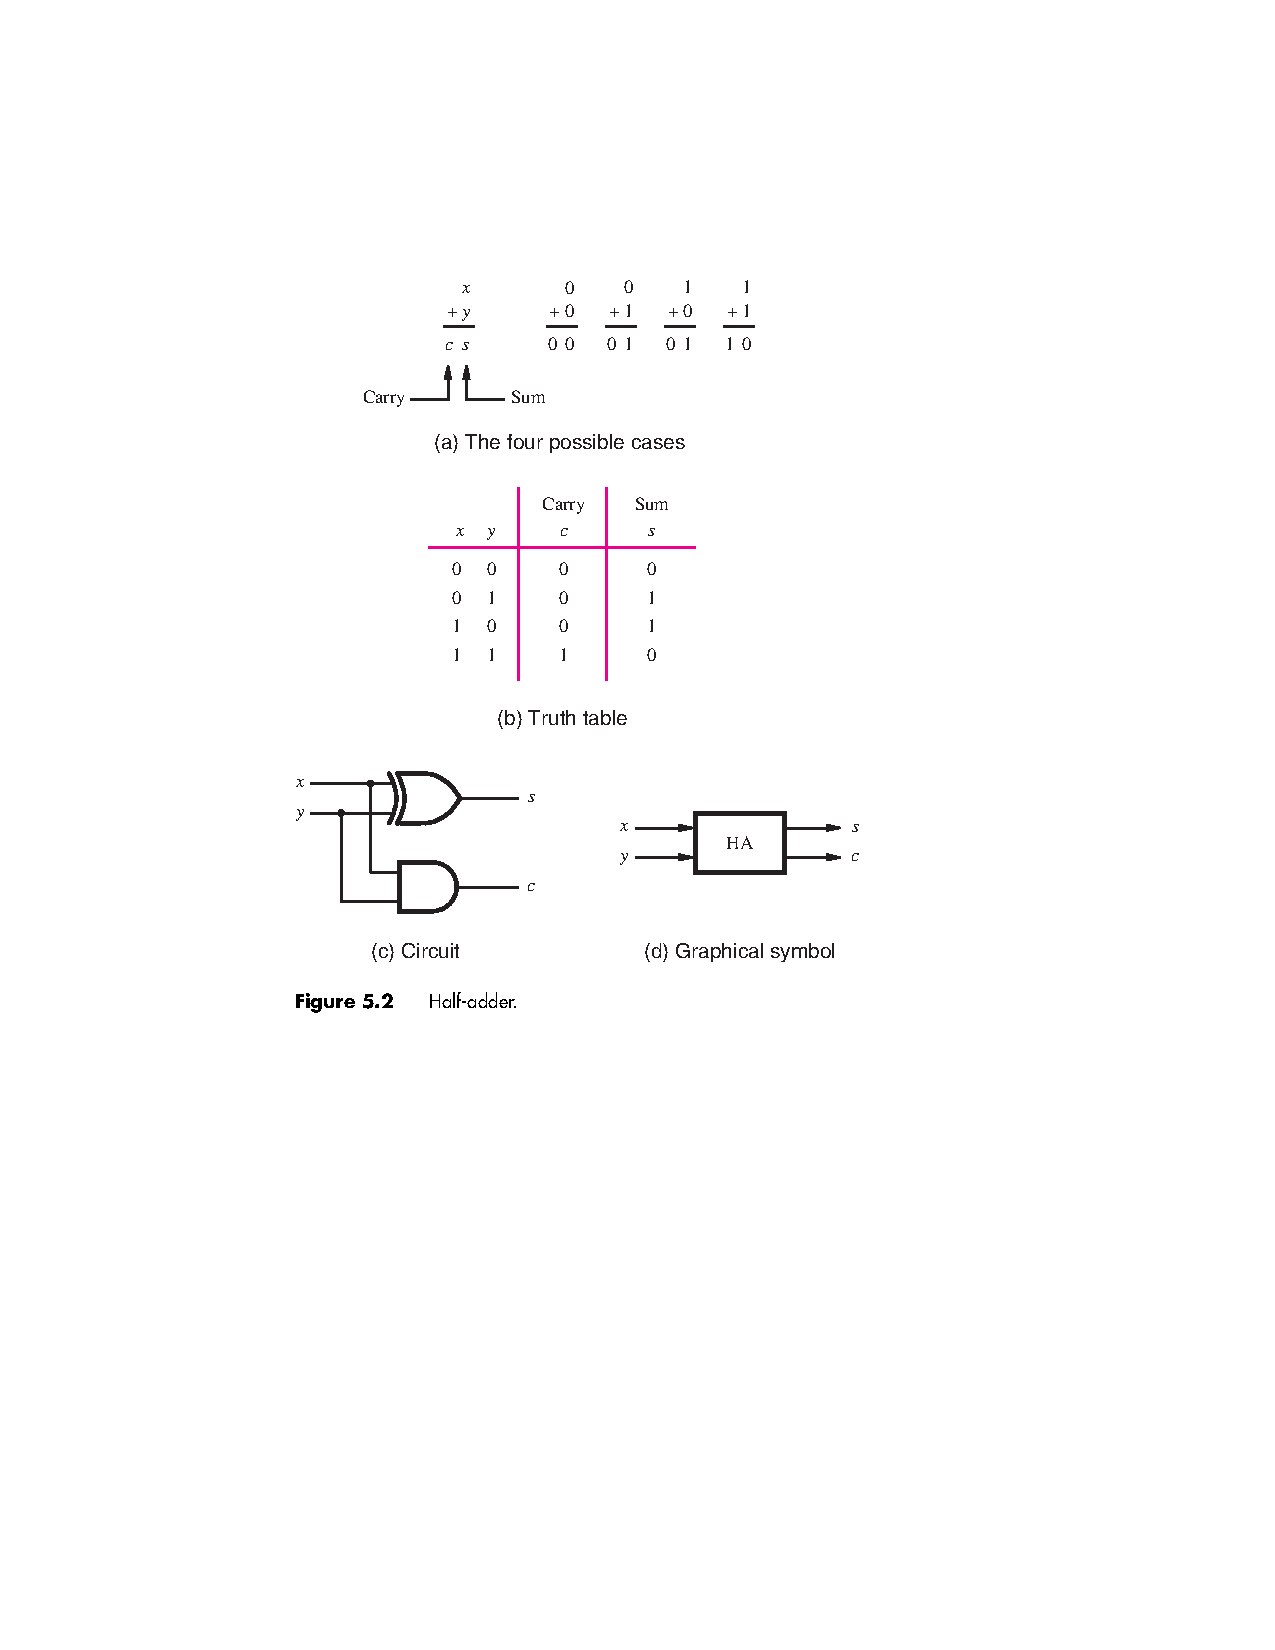
\includegraphics[scale=.6]{figs/VerilogFig5_2}
}

\frame{
    \frametitle{Adição Completa}
    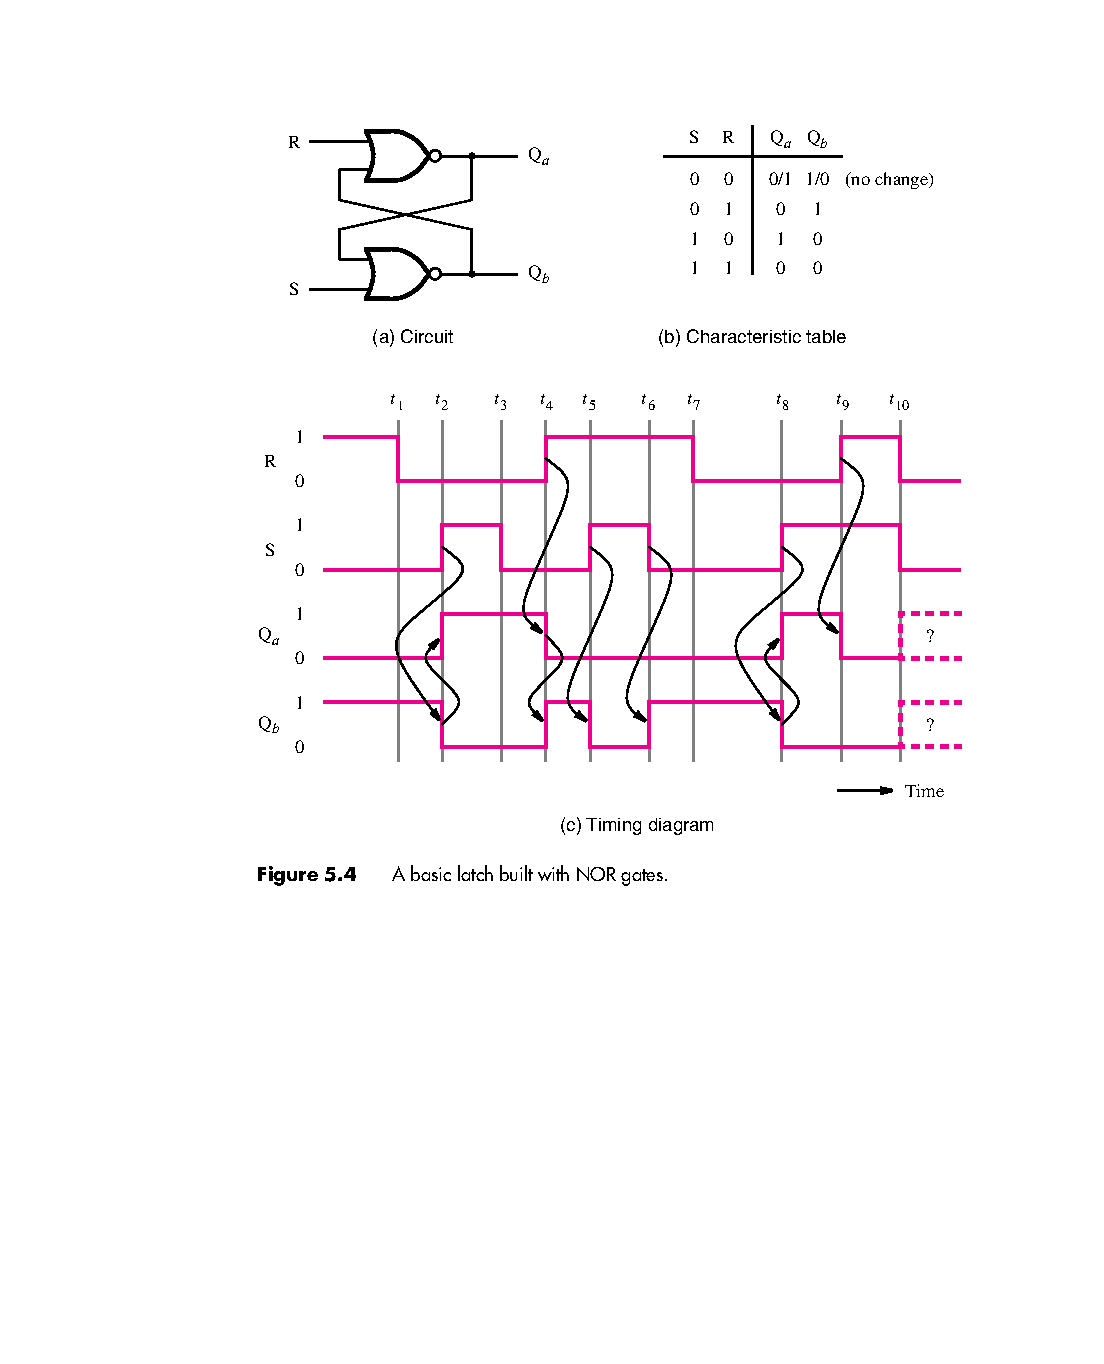
\includegraphics[scale=.5]{figs/VerilogFig5_4}
}

\frame{
    \frametitle{Números com Sinal}
    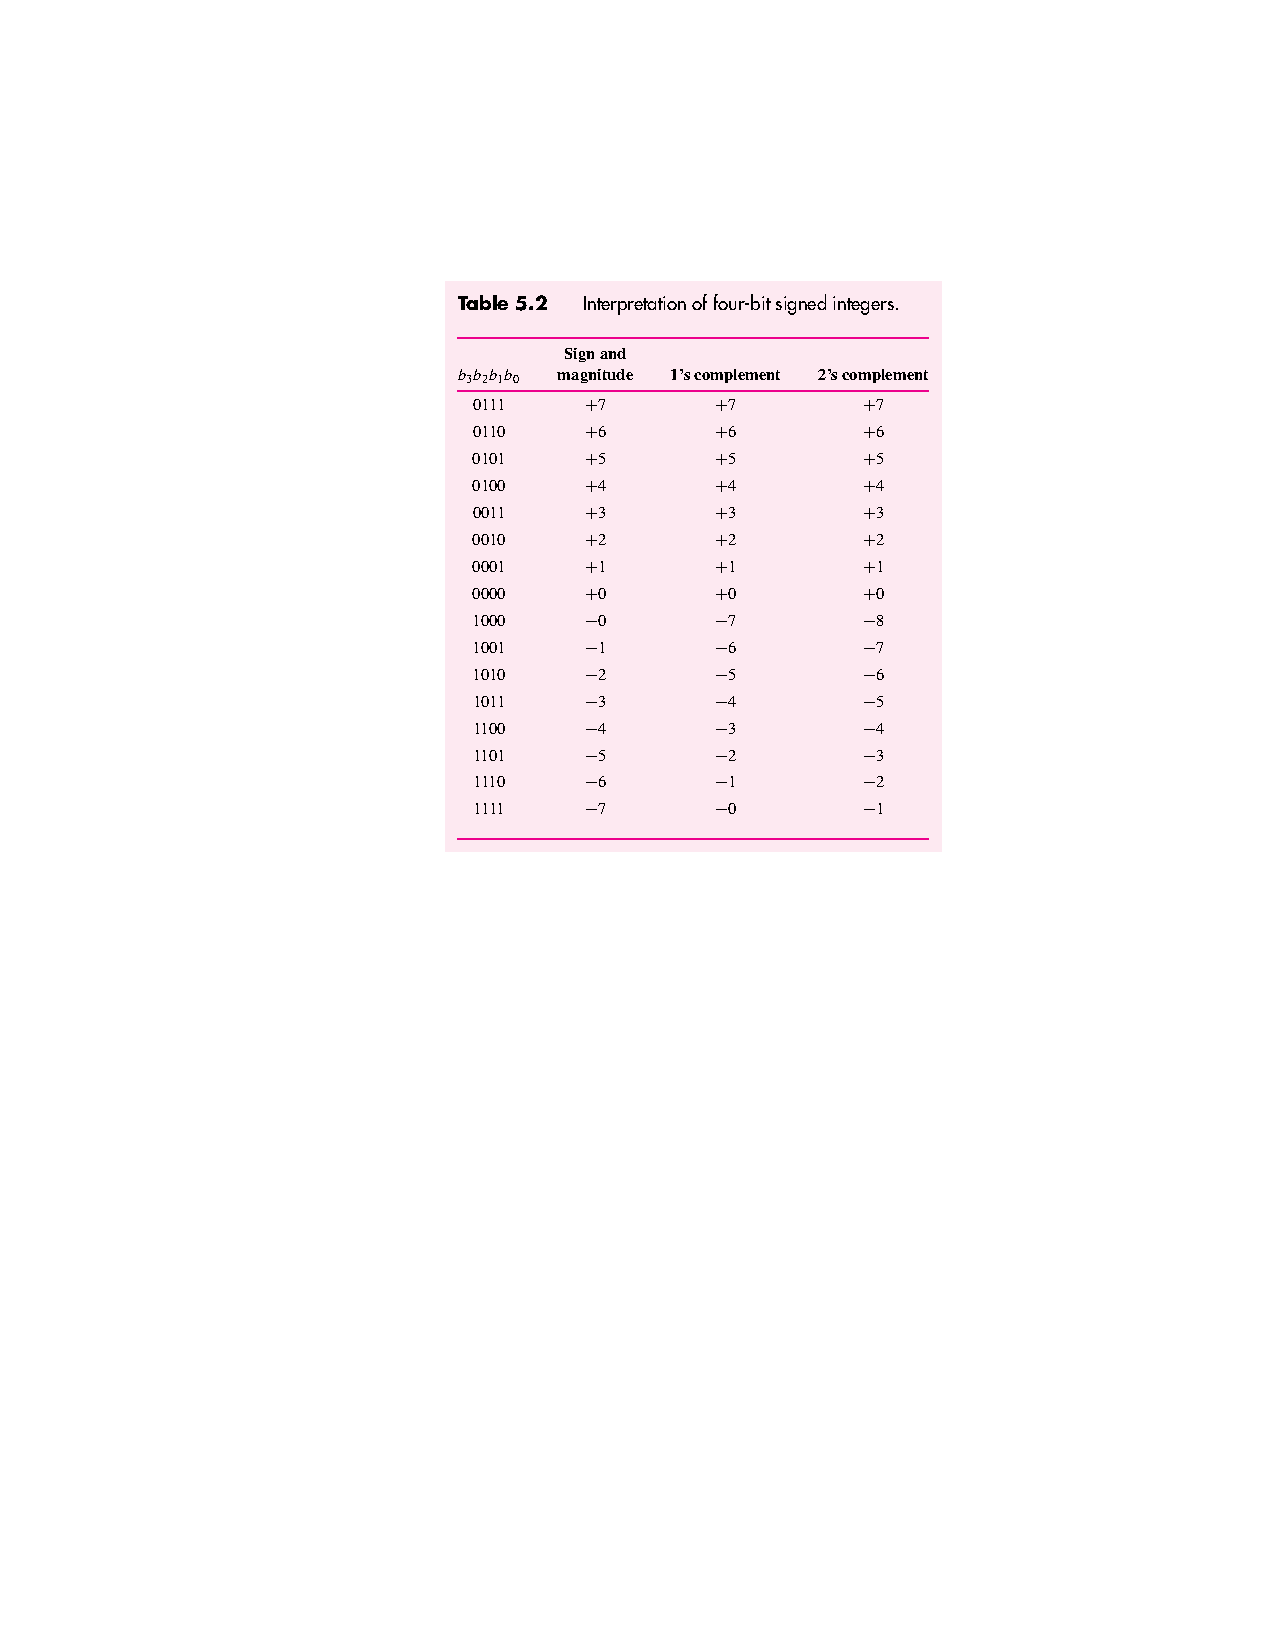
\includegraphics[scale=.7]{figs/VerilogTab5_2}
}

\frame{
    \frametitle{Soma em Complemento de Dois}
    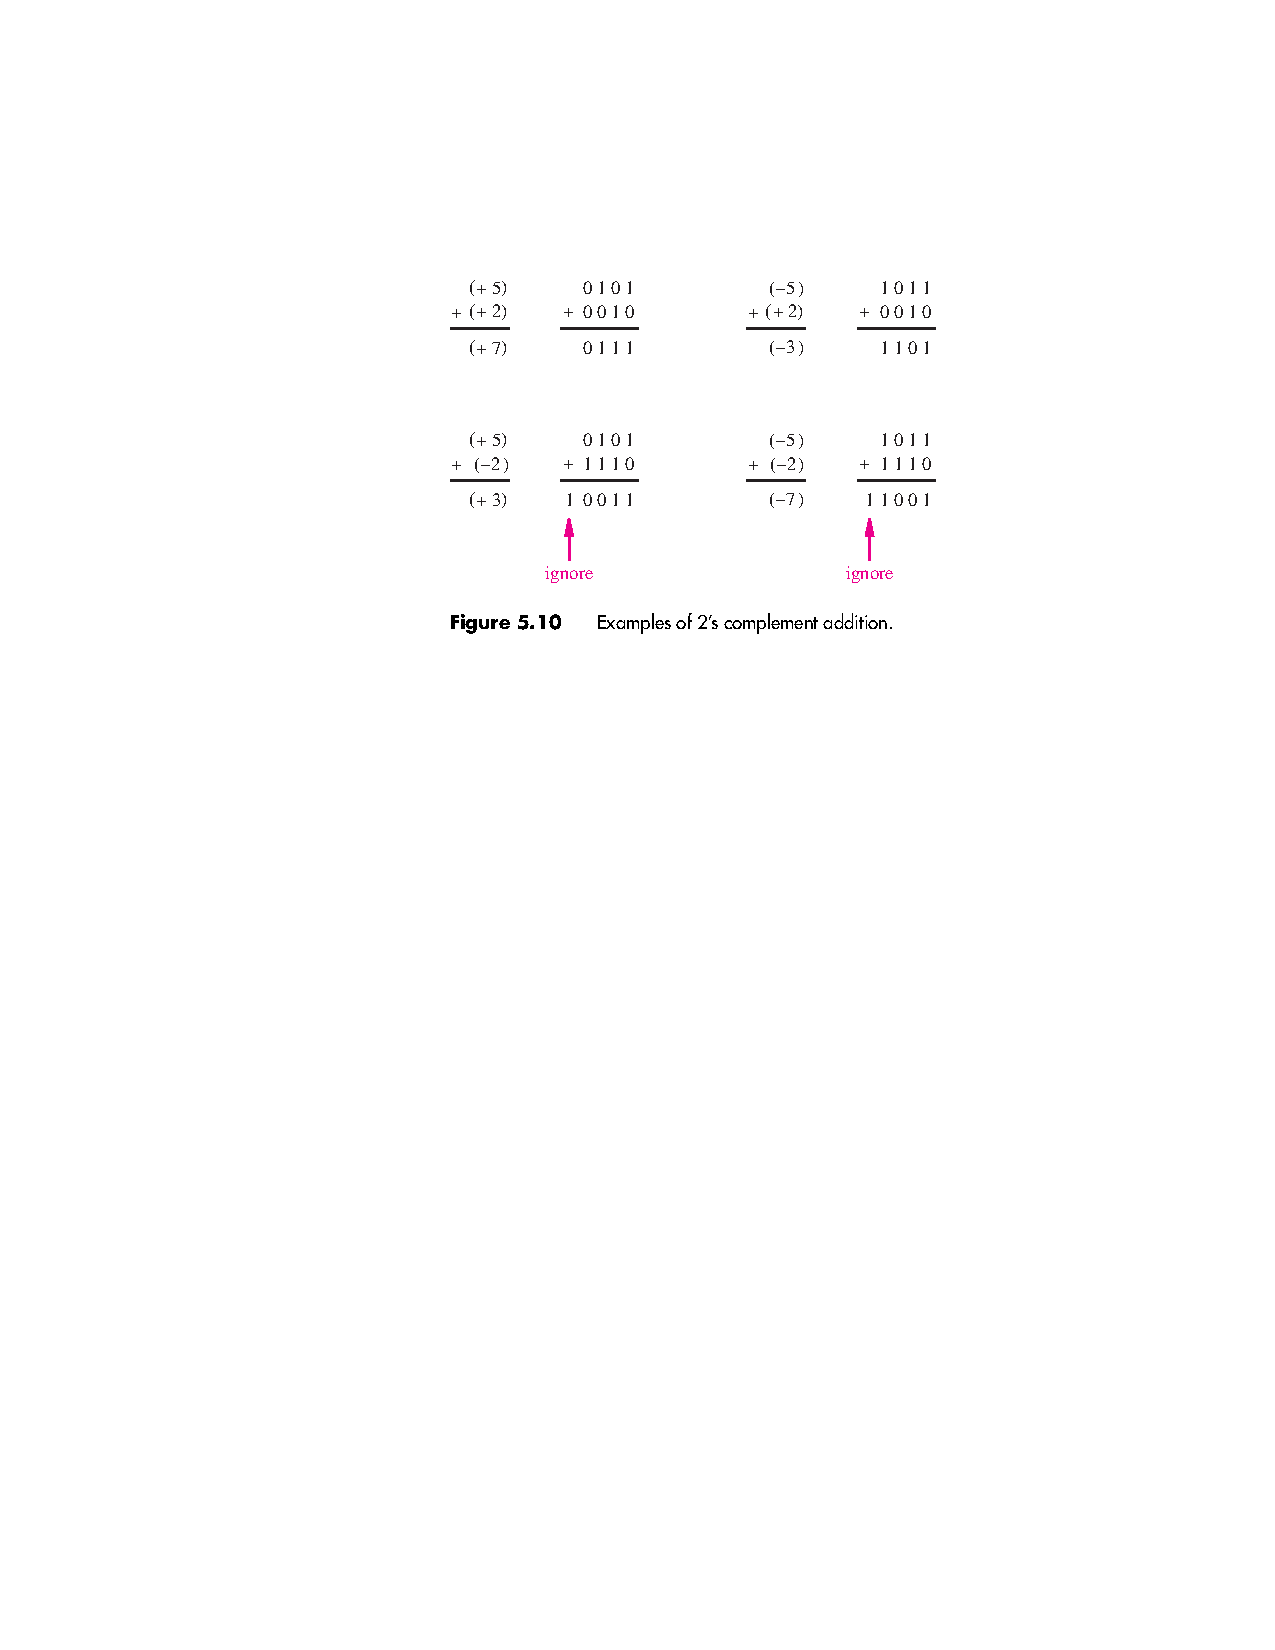
\includegraphics[scale=.7]{figs/VerilogFig5_10}
}

\frame{
    \frametitle{Somador/Subtrator}
    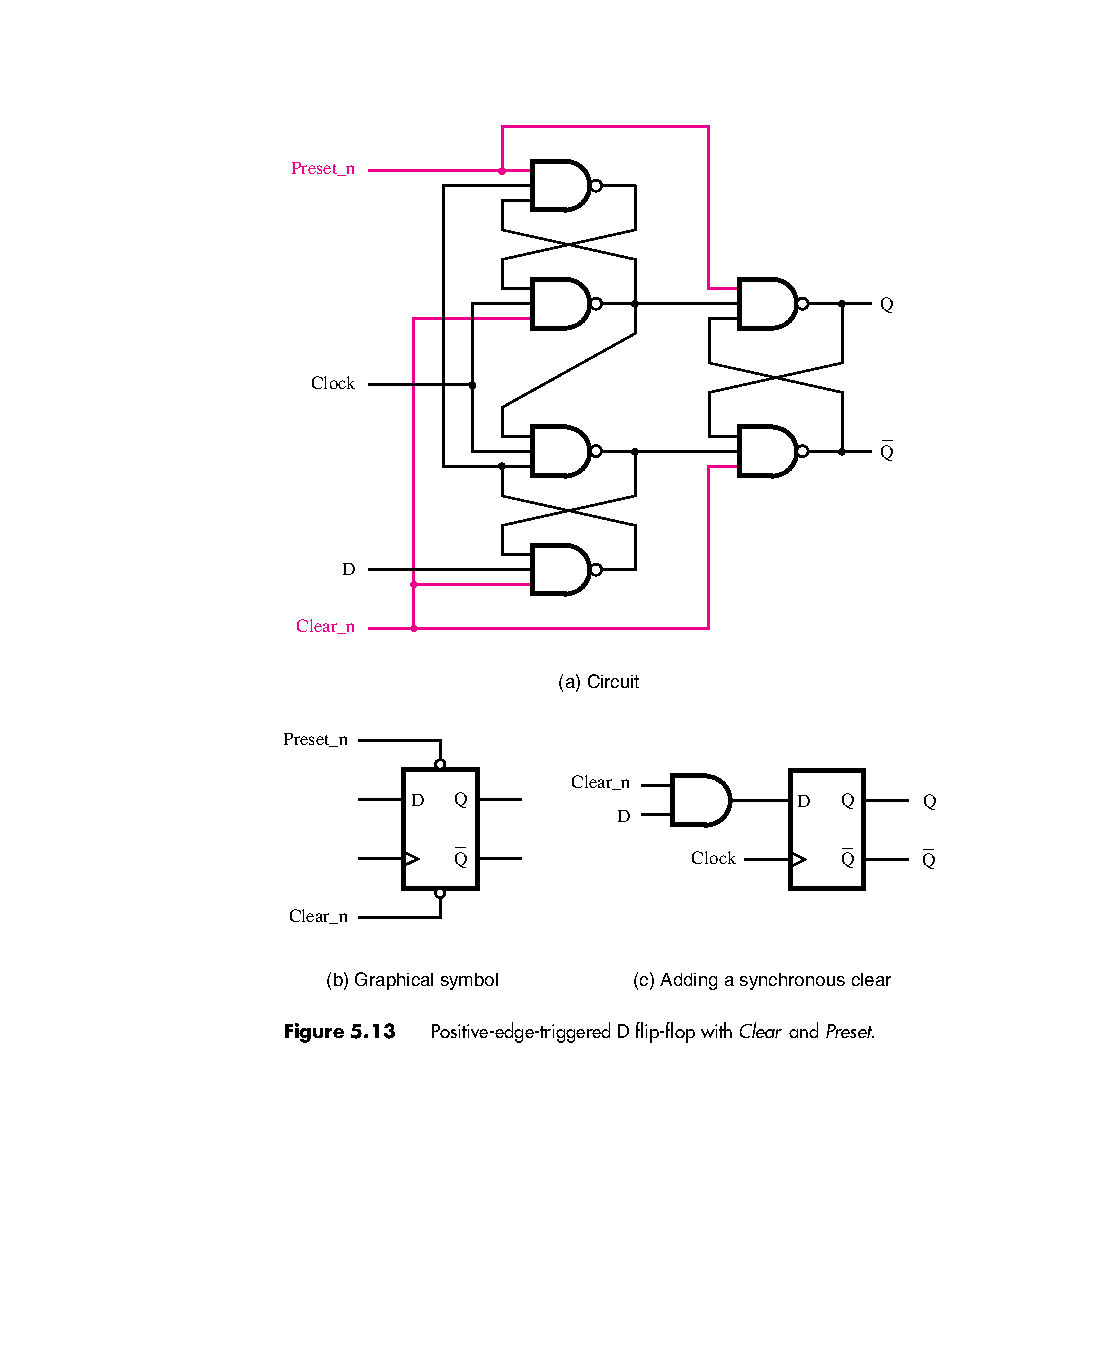
\includegraphics[scale=.7]{figs/VerilogFig5_13}
}

\frame{
    \frametitle{Detecção de Overflow}
    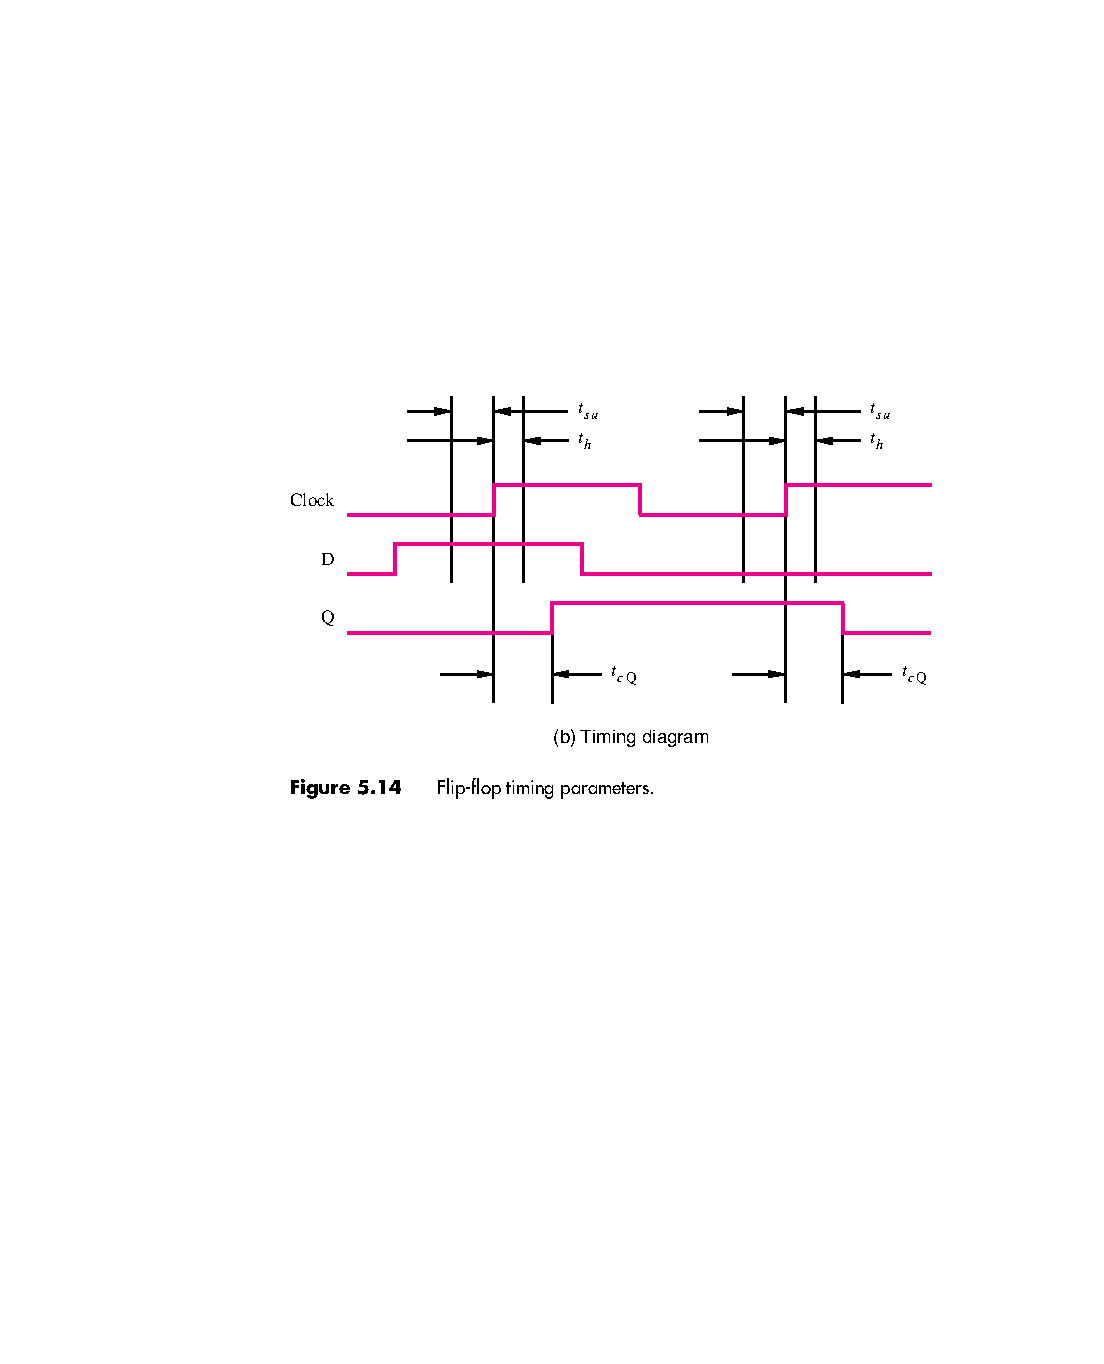
\includegraphics[scale=.7]{figs/VerilogFig5_14}
}

\subsection{Implementação (I)} 

\begin{frame}[fragile]
	\frametitle{Somador Completo usando primitivas}
	\begin{verilogcode}
module fulladd (Cin, x, y, s, Cout); 
  input Cin, x, y;
  output s, Cout;

  xor (s, x, y, Cin); 
  and (z1, x, y);
  and (z2, x, Cin); 
  and (z3, y, Cin);
  or (Cout, z1, z2, z3);
endmodule
	\end{verilogcode} 
\end{frame}

\begin{frame}[fragile]
	\frametitle{Sintaxe alternativa}
	\begin{verilogcode}
module fulladd (Cin, x, y, s, Cout); 
  input Cin, x, y;
  output s, Cout;

  xor (s, x, y, Cin); 
  and (z1, x, y),
      (z2, x, Cin),
      (z3, y, Cin);
  or (Cout, z1, z2, z3);
endmodule	
    \end{verilogcode} 
\end{frame}

\begin{frame}[fragile]
	\frametitle{Somador Completo usando Atribuições Contínuas}
	\begin{verilogcode}
module fulladd (Cin, x, y, s, Cout); 
  input Cin, x, y;
  output s, Cout;

  assign s = x ^ y ^ Cin;
  assign Cout = (x & y) | (x & Cin) | (y & Cin);
endmodule
    \end{verilogcode} 
\end{frame}

\begin{frame}[fragile]
	\frametitle{Sintaxe alternativa}
	\begin{verilogcode}
module fulladd (Cin, x, y, s, Cout); 
  input Cin, x, y;
  output s, Cout;

  assign s = x ^ y ^ Cin,
         Cout = (x & y) | (x & Cin) | (y & Cin);
endmodule
	\end{verilogcode} 
\end{frame}

\begin{frame}[fragile]
	\frametitle{Somador de 4 bits}
	\begin{verilogcode}
module adder4 (carryin, x3, x2, x1, x0, 
                        y3, y2, y1, y0, 
                        s3, s2, s1, s0, carryout); 
  input carryin, x3, x2, x1, x0, y3, y2, y1, y0;
  output s3, s2, s1, s0, carryout;

  fulladd stage0 (carryin, x0, y0, s0, c1); 
  fulladd stage1 (c1, x1, y1, s1, c2); 
  fulladd stage2 (c2, x2, y2, s2, c3); 
  fulladd stage3 (c3, x3, y3, s3, carryout);
endmodule	
	\end{verilogcode} 
\end{frame}

\begin{frame}[fragile]
	\frametitle{Somador de 4 bits}
	\begin{verilogcode}
module adder4 (carryin, x3, x2, x1, x0, 
                        y3, y2, y1, y0, 
                        s3, s2, s1, s0, carryout); 
  input carryin, x3, x2, x1, x0, y3, y2, y1, y0;
  output s3, s2, s1, s0, carryout;

  fulladd stage0 (.x(x0), .y(y0), .s(s0), .Cout(c1)); 
  fulladd stage1 (c1, x1, y1, s1, c2); 
  fulladd stage2 (c2, x2, y2, s2, c3); 
  fulladd stage3 (c3, x3, y3, s3, carryout);
endmodule	
	\end{verilogcode} 
\end{frame}

\begin{frame}[fragile]
	\frametitle{Usando vetores}
	\begin{verilogcode}
module adder4 (carryin, X, Y, S, carryout); 
  input carryin;
  input [3:0] X, Y;
  output [3:0] S;
  output carryout; 
  wire [3:1] C;
  
  fulladd stage0 (carryin, X[0], Y[0], S[0], C[1]); 
  fulladd stage1 (C[1], X[1], Y[1], S[1], C[2]); 
  fulladd stage2 (C[2], X[2], Y[2], S[2], C[3]); 
  fulladd stage3 (C[3], X[3], Y[3], S[3], carryout);
endmodule	
	\end{verilogcode} 
\end{frame}

\begin{frame}[fragile]
	\frametitle{Especificação Genérica}
	\begin{verilogcode}
module addern (carryin, X, Y, S, carryout); 
  parameter n = 32;
  input carryin;
  input [n-1:0] X, Y;
  output [n-1:0] S; 
  output carryout; 
  reg[n-1:0]S; 
  reg carryout;
  reg [n:0] C; 
  integer k;
  
  always @(X or Y or carryin) 
  begin
    C[0] = carryin;
    for (k = 0; k < n; k = k+1) 
    begin
      S[k] = X[k] ^ Y[k] ^ C[k];
      C[k+1] = (X[k] & Y[k]) | (X[k] & C[k]) | (Y[k] & C[k]); 
    end
    carryout = C[n];
  end 
endmodule
	\end{verilogcode} 
\end{frame}

\begin{frame}[fragile]
	\frametitle{Usando atribuição aritmética}
	\begin{verilogcode}
module addern (carryin, X, Y, S); 
  parameter n = 32;
  input carryin;
  input [n-1:0] X, Y;
  output [n-1:0] S; 
  reg [n-1:0] S;

  always @(X or Y or carryin) 
    S = X + Y + carryin;
endmodule
	\end{verilogcode} 
\end{frame}

\begin{frame}[fragile]
	\frametitle{Calculando Carry-out e Overflow}
	\begin{verilogcode}
module addern (carryin, X, Y, S, carryout, overflow); 
  parameter n = 32;
  input carryin;
  input [n-1:0] X, Y;
  output [n-1:0] S;
  output carryout, overflow; 
  reg[n-1:0]S;
  reg carryout, overflow;

  always @(X or Y or carryin) 
  begin
    S = X + Y + carryin;
    carryout=(X[n-1] & Y[n-1]) | (X[n-1] & S[n-1]) 
                               | (Y[n-1] & S[n-1]); 
    overflow = carryout ^ X[n-1] ^ Y[n-1] ^ S[n-1];
  end 
endmodule
	\end{verilogcode} 
\end{frame}

\begin{frame}[fragile]
	\frametitle{Sintaxe alternativa}
	\begin{verilogcode}
module addern (carryin, X, Y, S, carryout, overflow); 
  parameter n = 32;
  input carryin;
  input [n-1:0] X, Y;
  output [n-1:0] S;
  output carryout, overflow; 
  reg [n-1:0] S;
  reg carryout, overflow;

  always @(X or Y or carryin) 
  begin
    {carryout, S} = X + Y + carryin;
    overflow = carryout ^ X[n-1] ^ Y[n-1] ^ S[n-1]; 
  end
endmodule	
	\end{verilogcode} 
\end{frame}

\section{Circuitos Combinacionais}

\subsection{Multiplexadores}

\frame{
    \frametitle{Multiplexadores}
    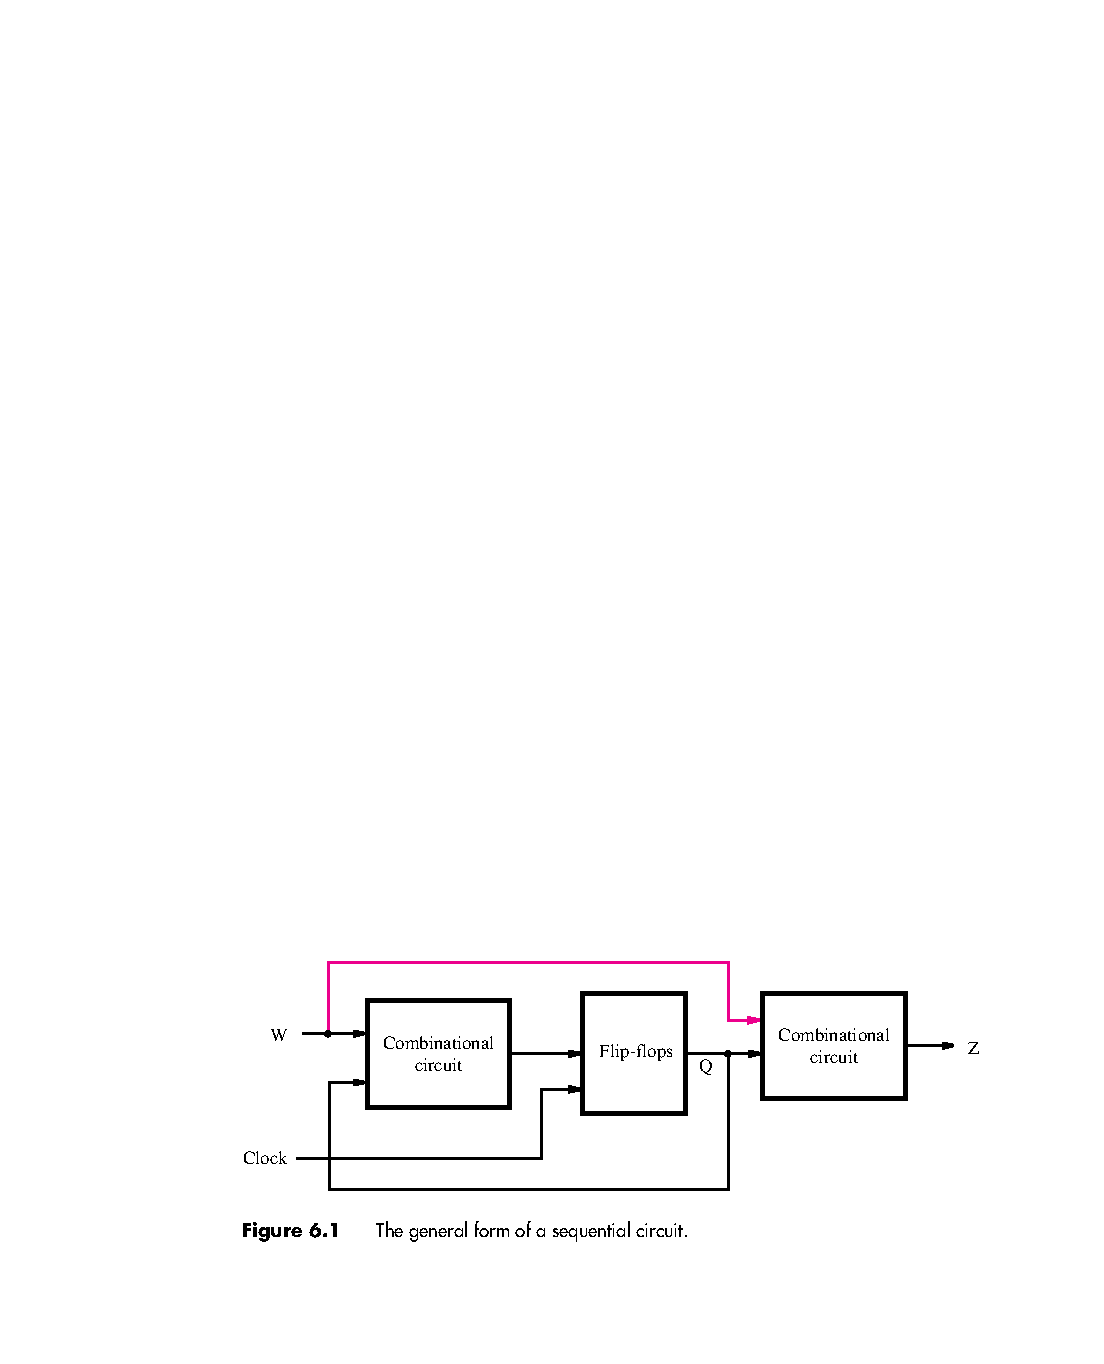
\includegraphics[scale=.7]{figs/VerilogFig6_1}
}

\begin{frame}[fragile]
	\frametitle{Multiplexador 2 para 1}
	\begin{verilogcode}
module mux2to1 (w0, w1, s, f); 
  input w0, w1, s;
  output f;

  assign f = s ? w1 : w0; 
endmodule
	\end{verilogcode} 
\end{frame}

\begin{frame}[fragile]
	\frametitle{Multiplexador 2 para 1}
	\begin{verilogcode}
module mux2to1 (w0, w1, s, f); 
  input w0, w1, s;
  output f;
  reg f;

  always @(w0 or w1 or s) 
    f = s ? w1 : w0;
endmodule
	\end{verilogcode} 
\end{frame}

\begin{frame}[fragile]
	\frametitle{Multiplexador 2 para 1}
	\begin{verilogcode}
module mux2to1 (w0, w1, s, f); 
  input w0, w1, s;
  output f;
  reg f;

  always @(w0 or w1 or s) 
    if (s == 0)
      f = w0;
    else
      f = w1;
endmodule
	\end{verilogcode} 
\end{frame}

\frame{
    \frametitle{Multiplexadores}
    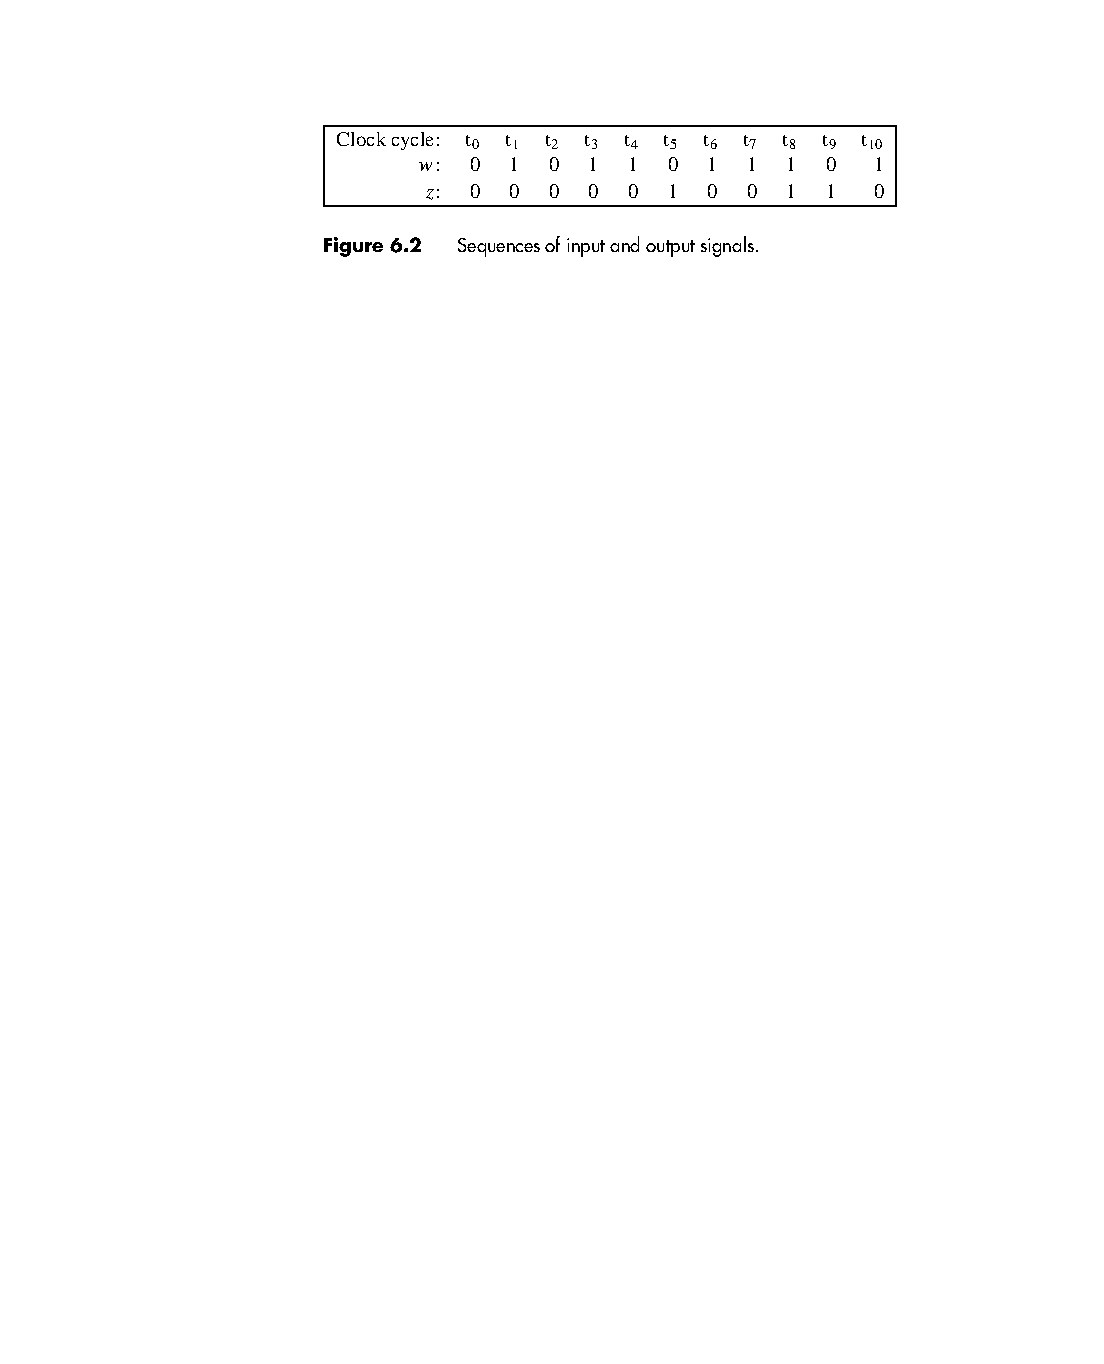
\includegraphics[scale=.7]{figs/VerilogFig6_2}
}

\begin{frame}[fragile]
	\frametitle{Multiplexador 4 para 1}
	\begin{verilogcode}
module mux4to1 (w0, w1, w2, w3, S, f);
  input w0, w1, w2, w3;
  input [1:0] S;
  output f;

  assign f = S[1] ? (S[0] ? w3 : w2) : (S[0] ? w1 : w0); 
endmodule
	\end{verilogcode} 
\end{frame}

\begin{frame}[fragile]
	\frametitle{Multiplexador 4 para 1}
	\begin{verilogcode}
module mux4to1 (w0, w1, w2, w3, S, f); 
  input w0, w1, w2, w3;
  input [1:0] S;
  output f;
  reg f;

  always @(w0 or w1 or w2 or w3 or S) 
    if (S == 2'b00)
      f = w0;
    else if (S == 2'b01)
      f = w1;
    else if (S == 2'b10)
      f = w2;
    else if (S == 2'b11)
      f = w3;
endmodule
	\end{verilogcode} 
\end{frame}

\begin{frame}[fragile]
	\frametitle{Multiplexador 4 para 1}
	\begin{verilogcode}
module mux4to1 (W, S, f); 
  input [0:3] W;
  input [1:0] S;
  output f;
  reg f;

  always @(W or S) 
    if (S == 0)
      f = W[0]; 
    else if (S == 1) 
      f = W[1]; 
    else if (S == 2)
      f = W[2]; 
    else if (S == 3) 
      f = W[3];
endmodule
    \end{verilogcode} 
\end{frame}



\begin{frame}[fragile]
	\frametitle{Multiplexador 4 para 1}
	\begin{verilogcode}
module mux4to1 (W, S, f); 
  input [0:3] W;
  input [1:0] S;
  output f;
  reg f;

  always @(W or S) 
    case (S)
      0: f = W[0]; 
      1: f = W[1]; 
      2: f = W[2]; 
      3: f = W[3];
    endcase 
endmodule
    \end{verilogcode} 
\end{frame}

\begin{frame}[fragile]
	\frametitle{Multiplexador 16 para 1}
	\begin{verilogcode}
module mux16to1 (W, S16, f); 
  input [0:15] W;
  input [3:0] S16;
  output f;
  wire [0:3] M;

  mux4to1 Mux1 (W[ 0: 3], S16[1:0], M[0]);
  mux4to1 Mux2 (W[ 4: 7], S16[1:0], M[1]);
  mux4to1 Mux3 (W[ 8:11], S16[1:0], M[2]);
  mux4to1 Mux4 (W[12:15], S16[1:0], M[3]);
  mux4to1 Mux5 (M[ 0: 3], S16[3:2], f);
endmodule
    \end{verilogcode} 
\end{frame}

\frame{
    \frametitle{Multiplexadores (Aplicação)}
    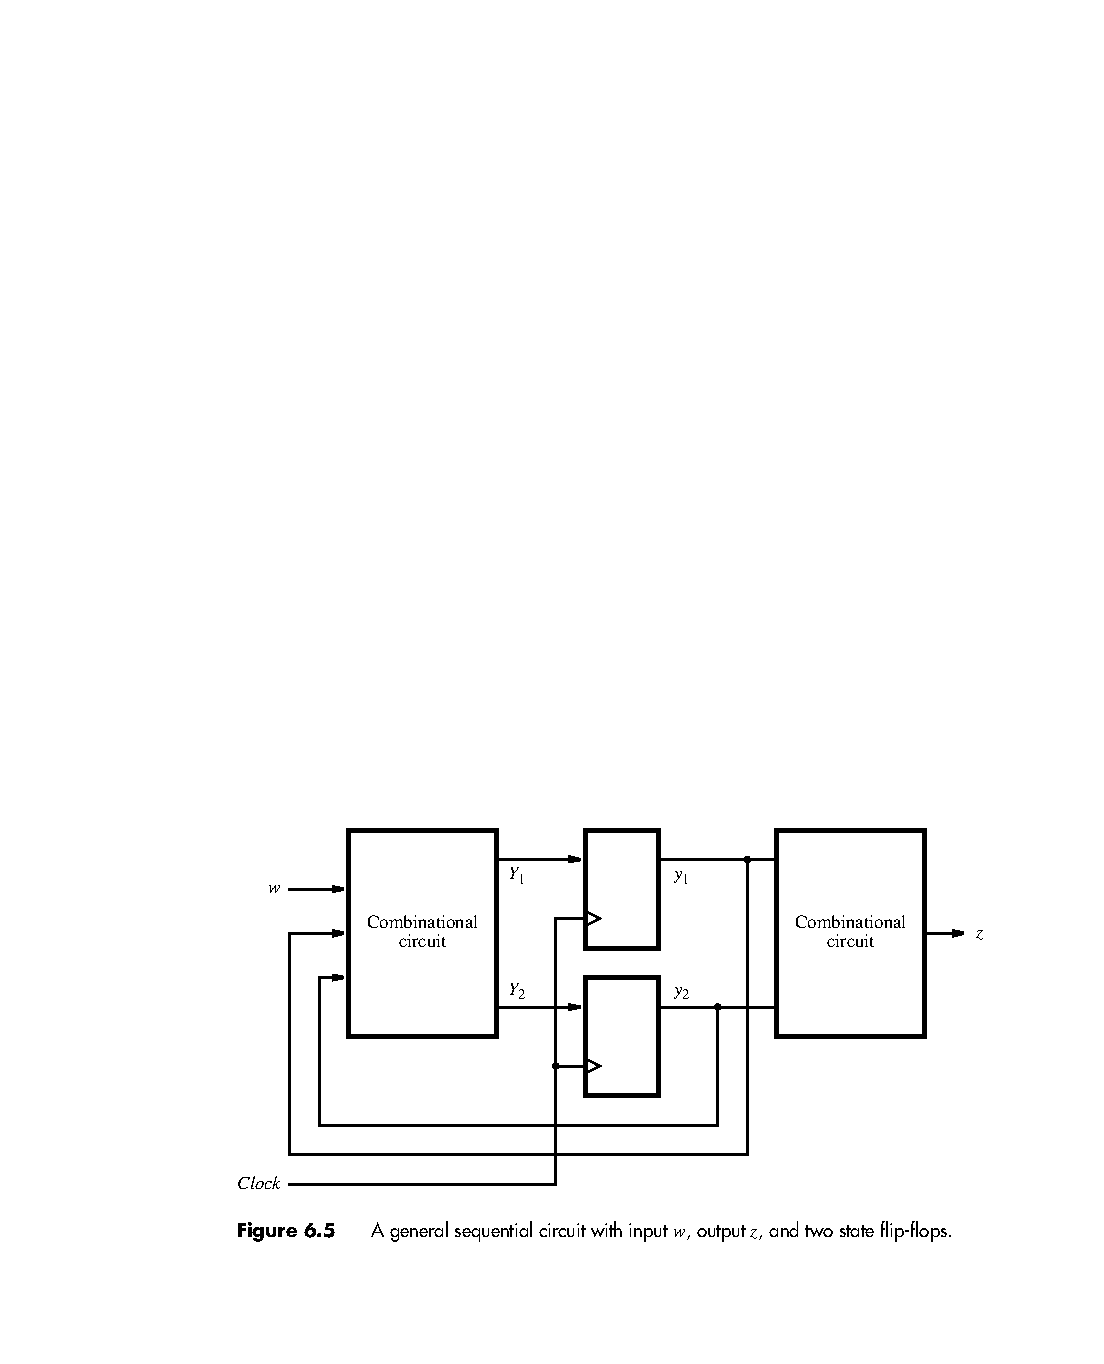
\includegraphics[scale=.7]{figs/VerilogFig6_5}
}


\subsection{Decodificadores}

\frame{
    \frametitle{Decodificadores}
    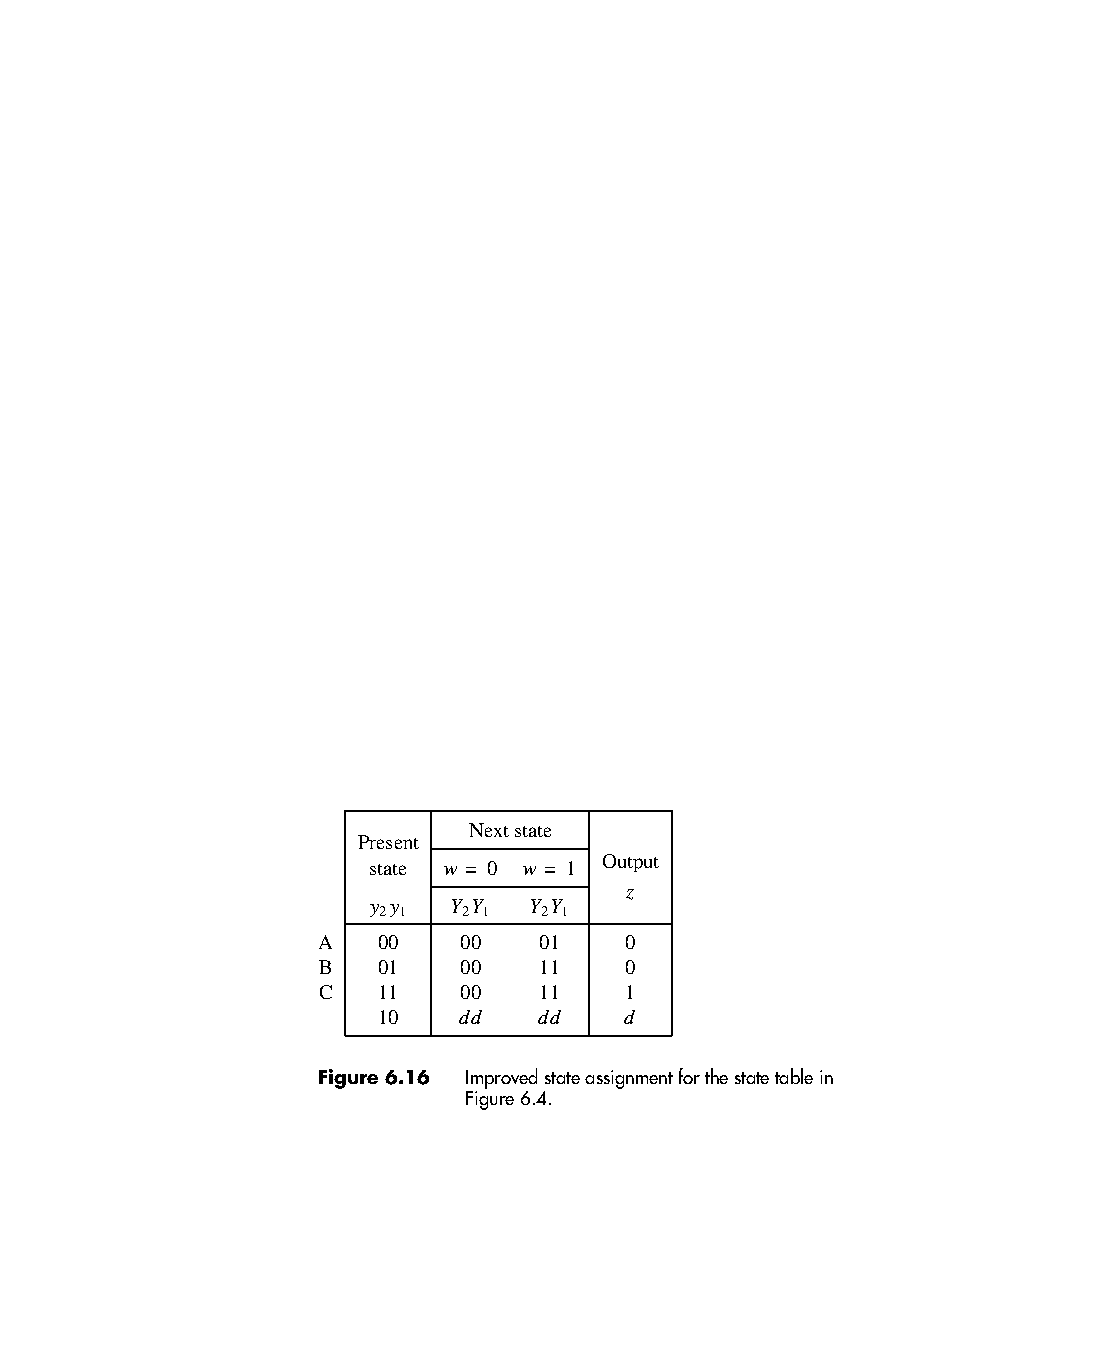
\includegraphics[scale=.6]{figs/VerilogFig6_16}
}

\begin{frame}[fragile]
	\frametitle{Multiplexador 16 para 1}
	\begin{verilogcode}
module dec2to4 (W, Y, En); 
  input [1:0] W;
  input En;
  output [0:3] Y;
  reg [0:3] Y;

  always @(W or En) 
    case ({En, W})
      3'b100: Y = 4'b1000; 
      3'b101: Y = 4'b0100; 
      3'b110: Y = 4'b0010; 
      3'b111: Y = 4'b0001; 
      default: Y = 4'b0000;
    endcase 
endmodule
    \end{verilogcode} 
\end{frame}

\begin{frame}[fragile]
	\frametitle{Multiplexador 16 para 1}
	\begin{verilogcode}
module dec2to4 (W, Y, En); 
  input [1:0] W;
  input En;
  output [0:3] Y;
  reg [0:3] Y;

  always @(W or En) 
  begin
    if (En == 0)
      Y = 4'b0000;
    else
      case (W)
        0: Y = 4'b1000; 
        1: Y = 4'b0100; 
        2: Y = 4'b0010; 
        3: Y = 4'b0001;
      endcase 
  end
endmodule
    \end{verilogcode} 
\end{frame}

\frame{
    \frametitle{Decodificadores}
    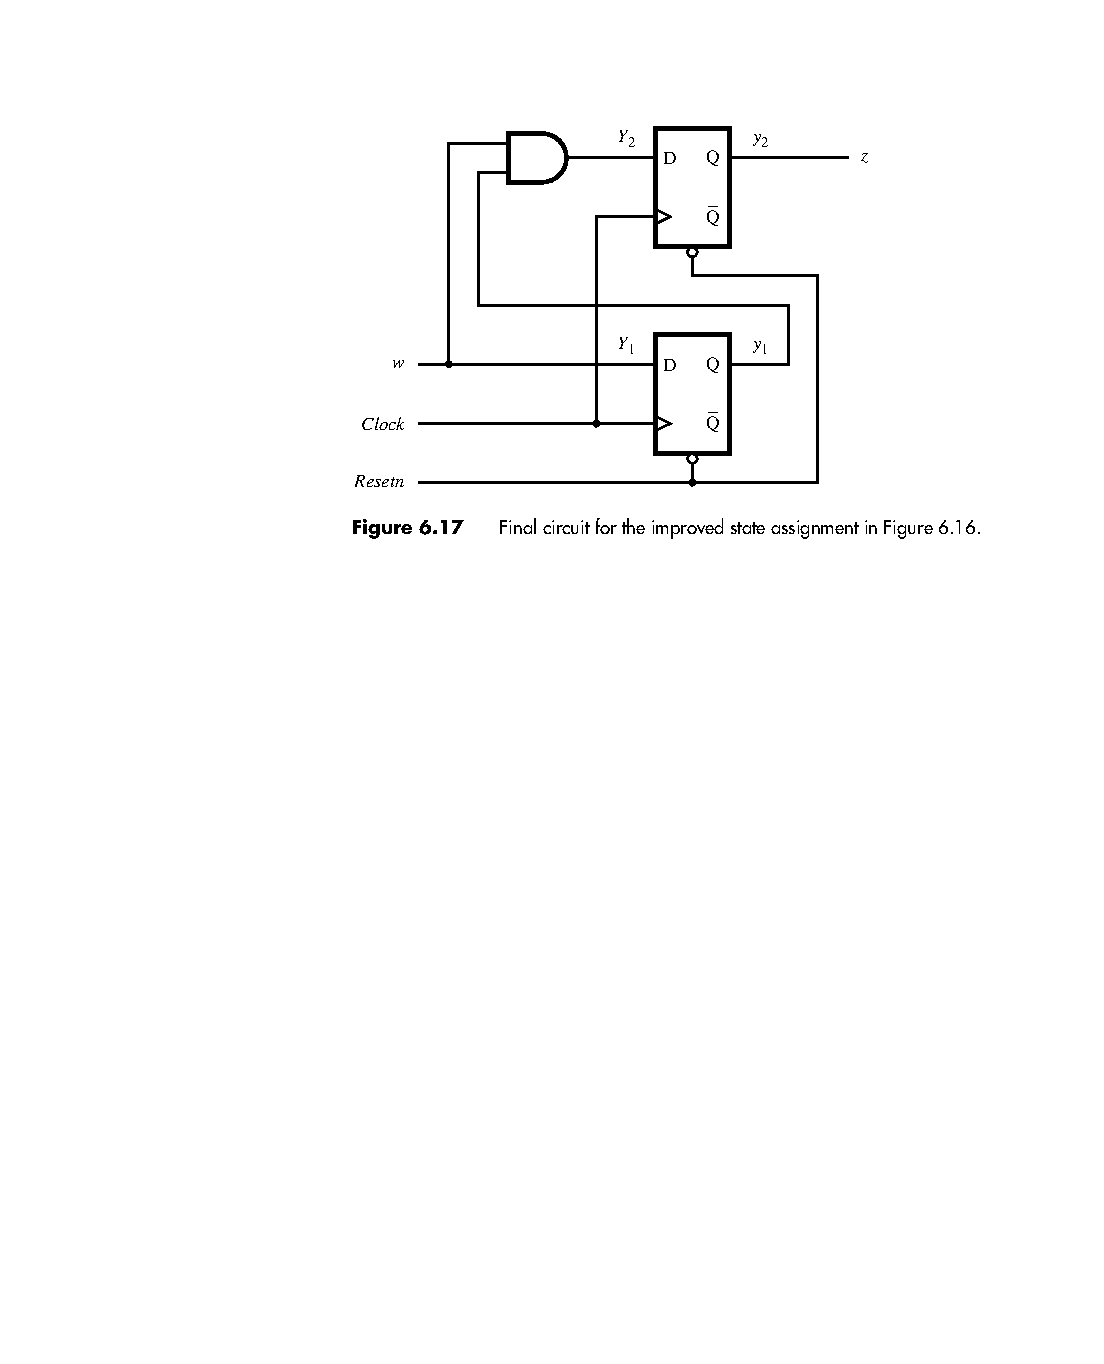
\includegraphics[scale=.7]{figs/VerilogFig6_17}
}

\frame{
    \frametitle{Decodificadores}
    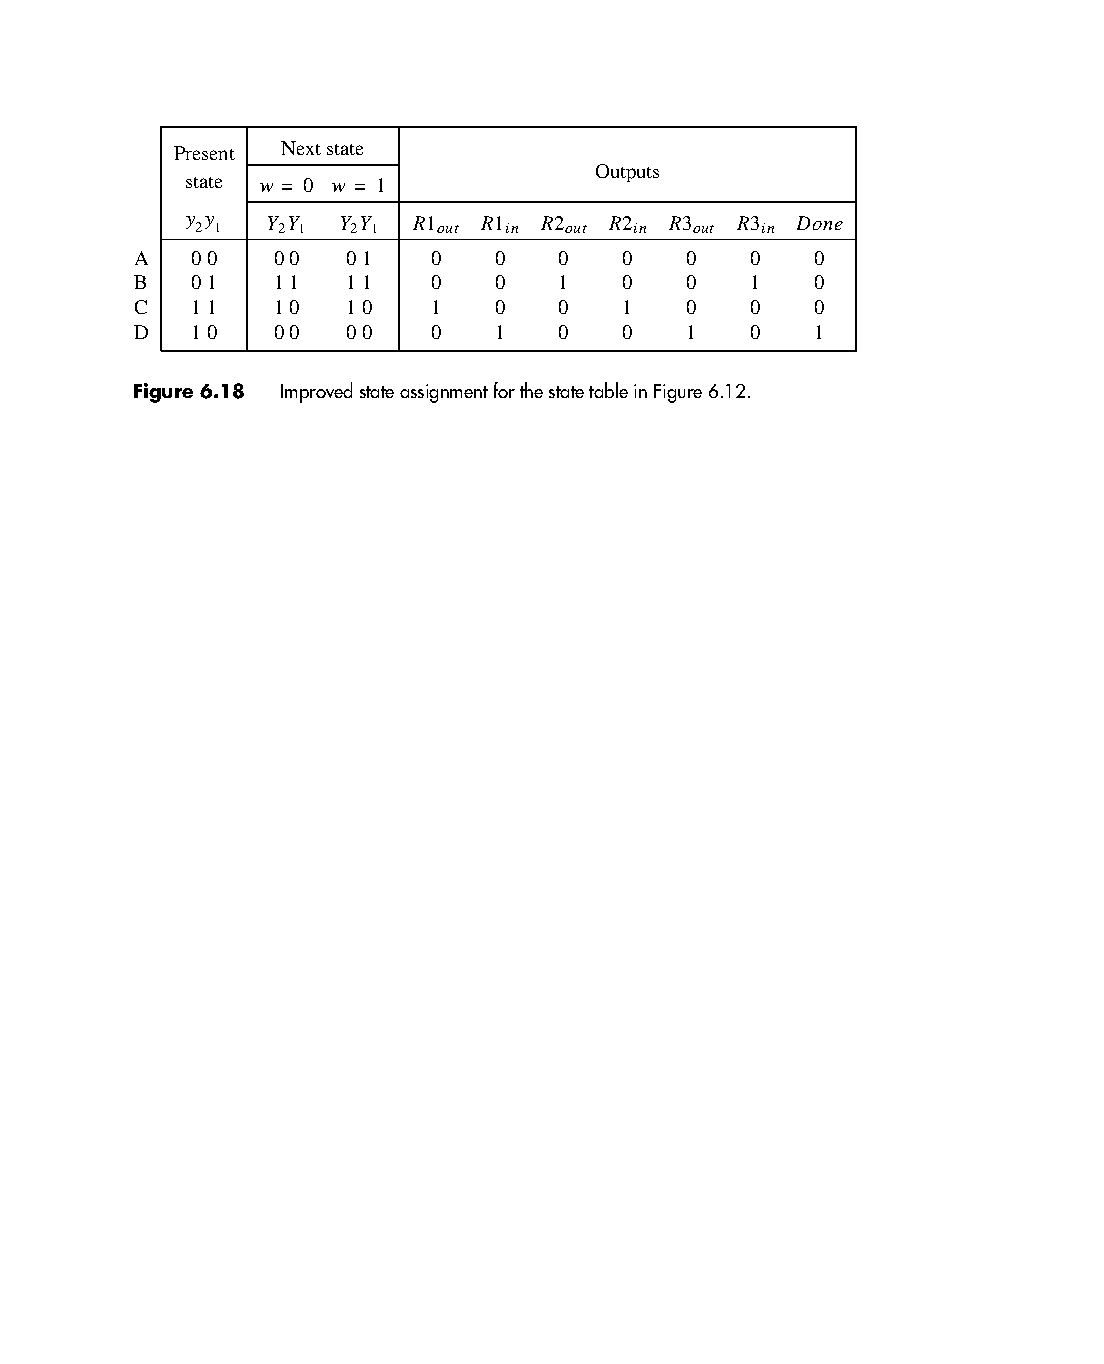
\includegraphics[scale=.7]{figs/VerilogFig6_18}
}

\begin{frame}[fragile]
	\frametitle{Decodificador 4 para 16}
	\begin{verilogcode}
module dec4to16 (W, Y, En); 
  input [3:0] W;
  input En;
  output [0:15] Y;
  wire [0:3] M;

  dec2to4 Dec1 (W[3:2], M[ 0: 3], En); 
  dec2to4 Dec2 (W[1:0], Y[ 0: 3], M[0]); 
  dec2to4 Dec3 (W[1:0], Y[ 4: 7], M[1]); 
  dec2to4 Dec4 (W[1:0], Y[ 8:11], M[2]); 
  dec2to4 Dec5 (W[1:0], Y[12:15], M[3]);
endmodule
    \end{verilogcode} 
\end{frame}

\subsection{Codificadores}

\frame{
    \frametitle{Codificadores}
    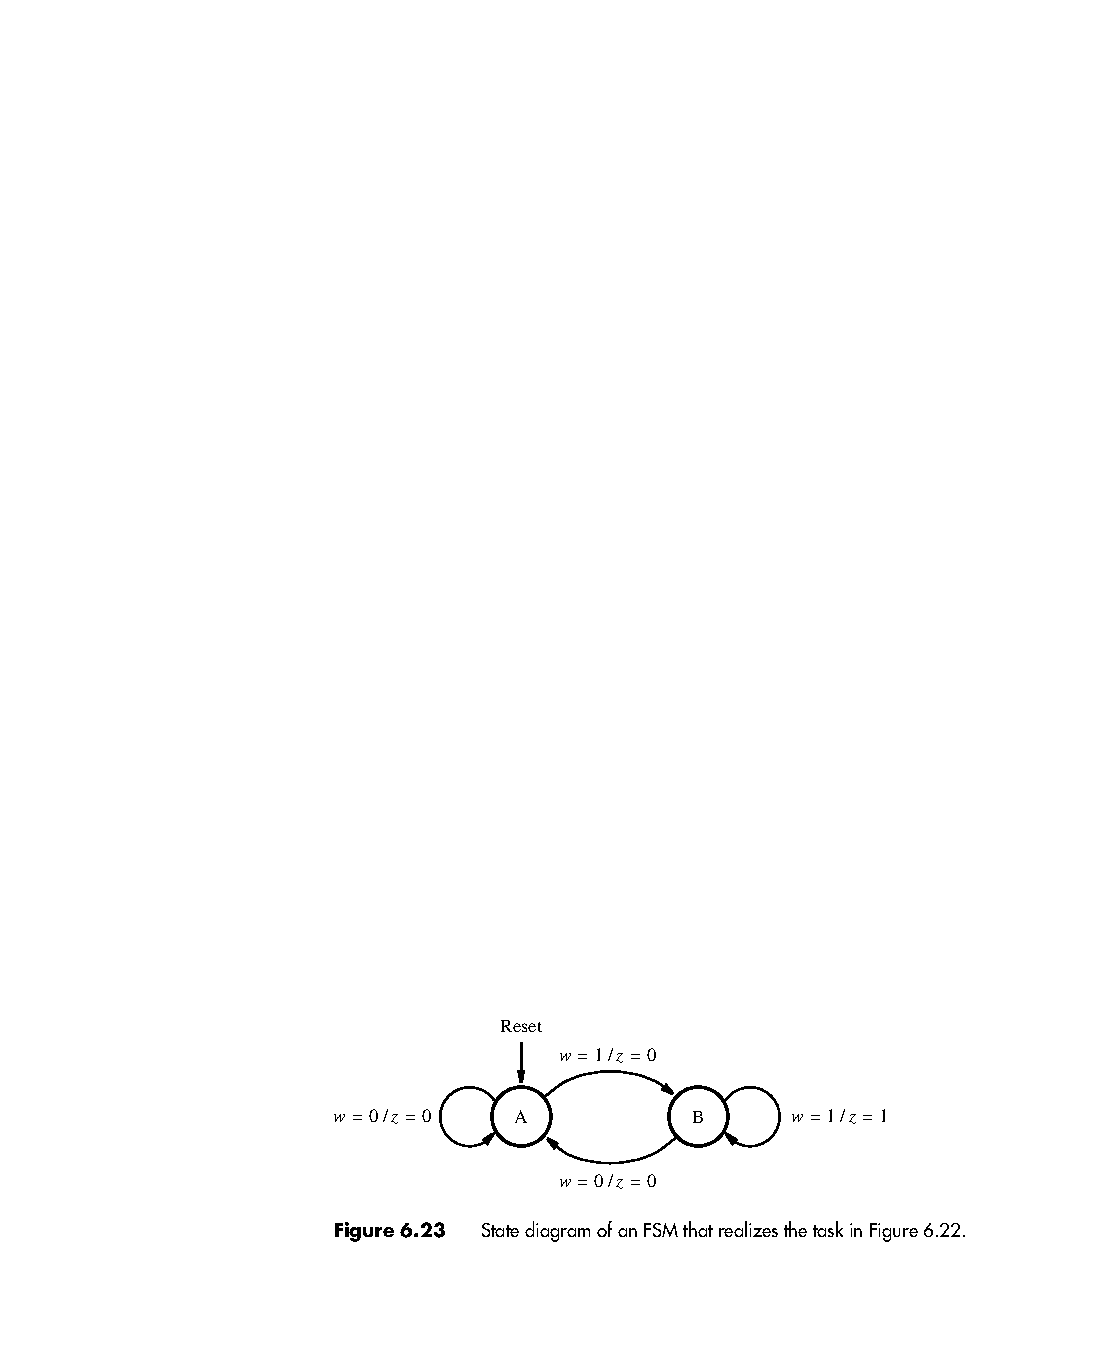
\includegraphics[scale=.7]{figs/VerilogFig6_23}
}

\begin{frame}[fragile]
	\frametitle{Codificador 4 para 2 (com prioridade)}
	\begin{verilogcode}
module priority (W, Y, z); 
  input [3:0] W;
  output [1:0] Y;
  output z;
  reg [1:0] Y; 
  reg z;

  always @(W) 
  begin
    z = 1; 
    casex (W)
      4'b1xxx: Y = 3;
      4'b01xx: Y = 2;
      4'b001x: Y = 1;
      4'b0001: Y = 0;
      default:
      begin
        z = 0;
        Y = 2'bx;
      end
    \end{verilogcode} 
\end{frame}

\subsection{Conversores}

\frame{
    \frametitle{Decodificador de 7 segmentos}
    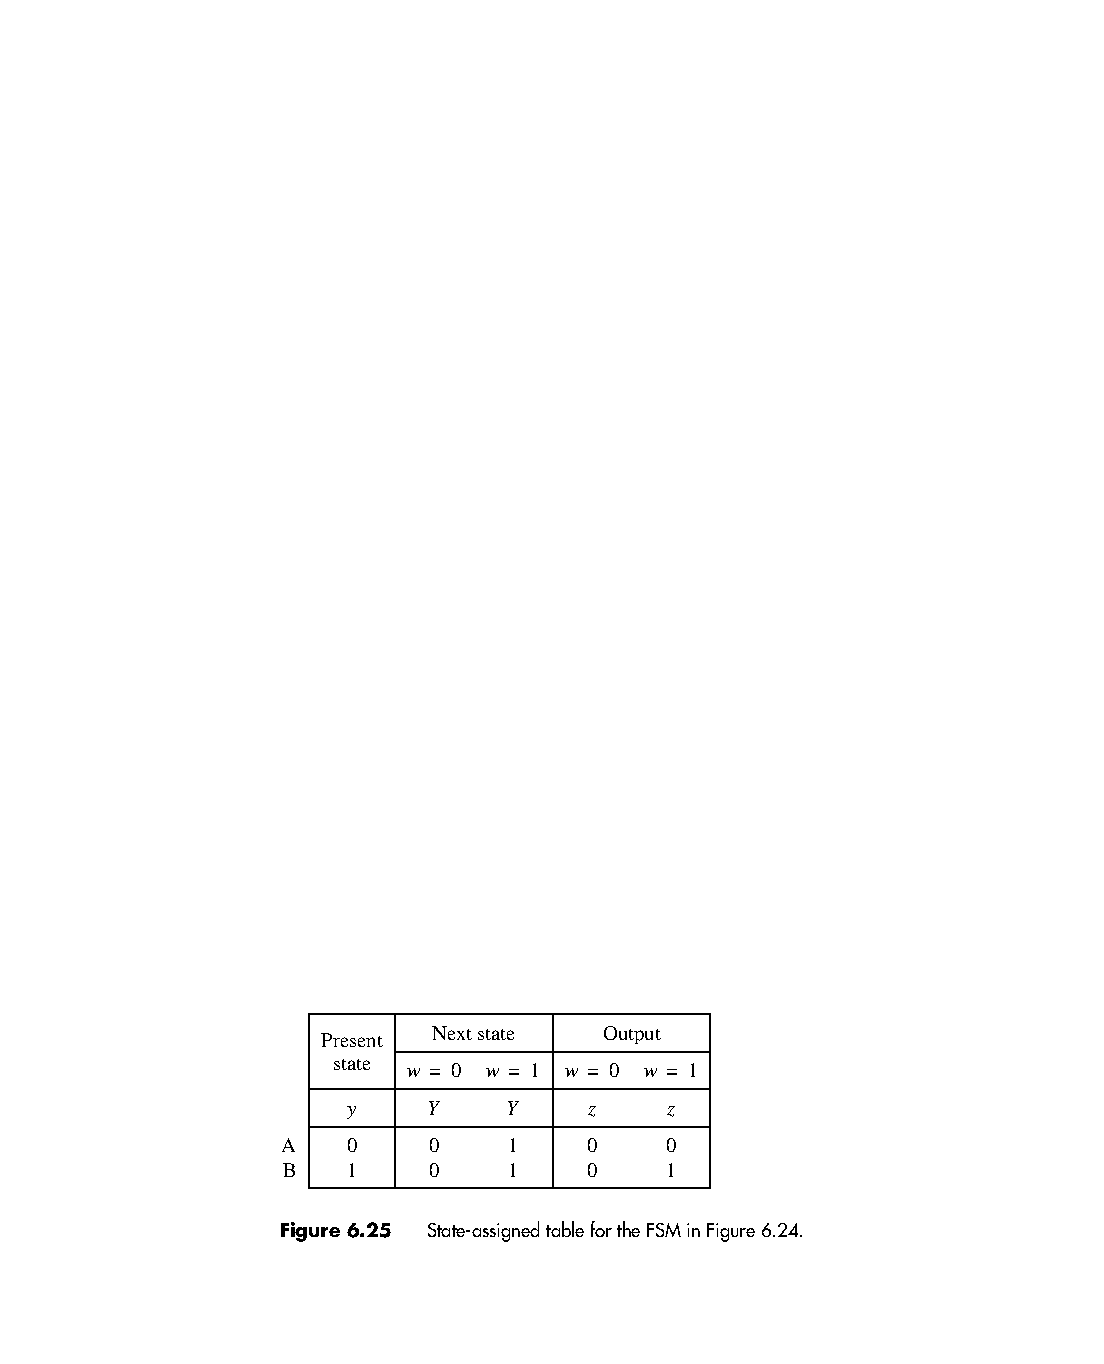
\includegraphics[scale=.7]{figs/VerilogFig6_25}
}

\begin{frame}[fragile]
	\frametitle{Decodificador de 7 segmentos}
	\begin{verilogcode}
module seg7 (bcd, leds); 
  input [3:0] bcd; 
  output [1:7] leds; 
  reg [1:7] leds;

  always @(bcd)
    case (bcd)   //abcdefg
      0: leds = 7'b1111110; 
      1: leds = 7'b0110000; 
      2: leds = 7'b1101101; 
      3: leds = 7'b1111001; 
      4: leds = 7'b0110011; 
      5: leds = 7'b1011011; 
      6: leds = 7'b1011111; 
      7: leds = 7'b1110000; 
      8: leds = 7'b1111111; 
      9: leds = 7'b1111011; 
      default: leds = 7'bx;
    endcase 
endmodule
    \end{verilogcode} 
\end{frame}

\subsection{Comparadores}

\frame{
    \frametitle{Comparadores}
    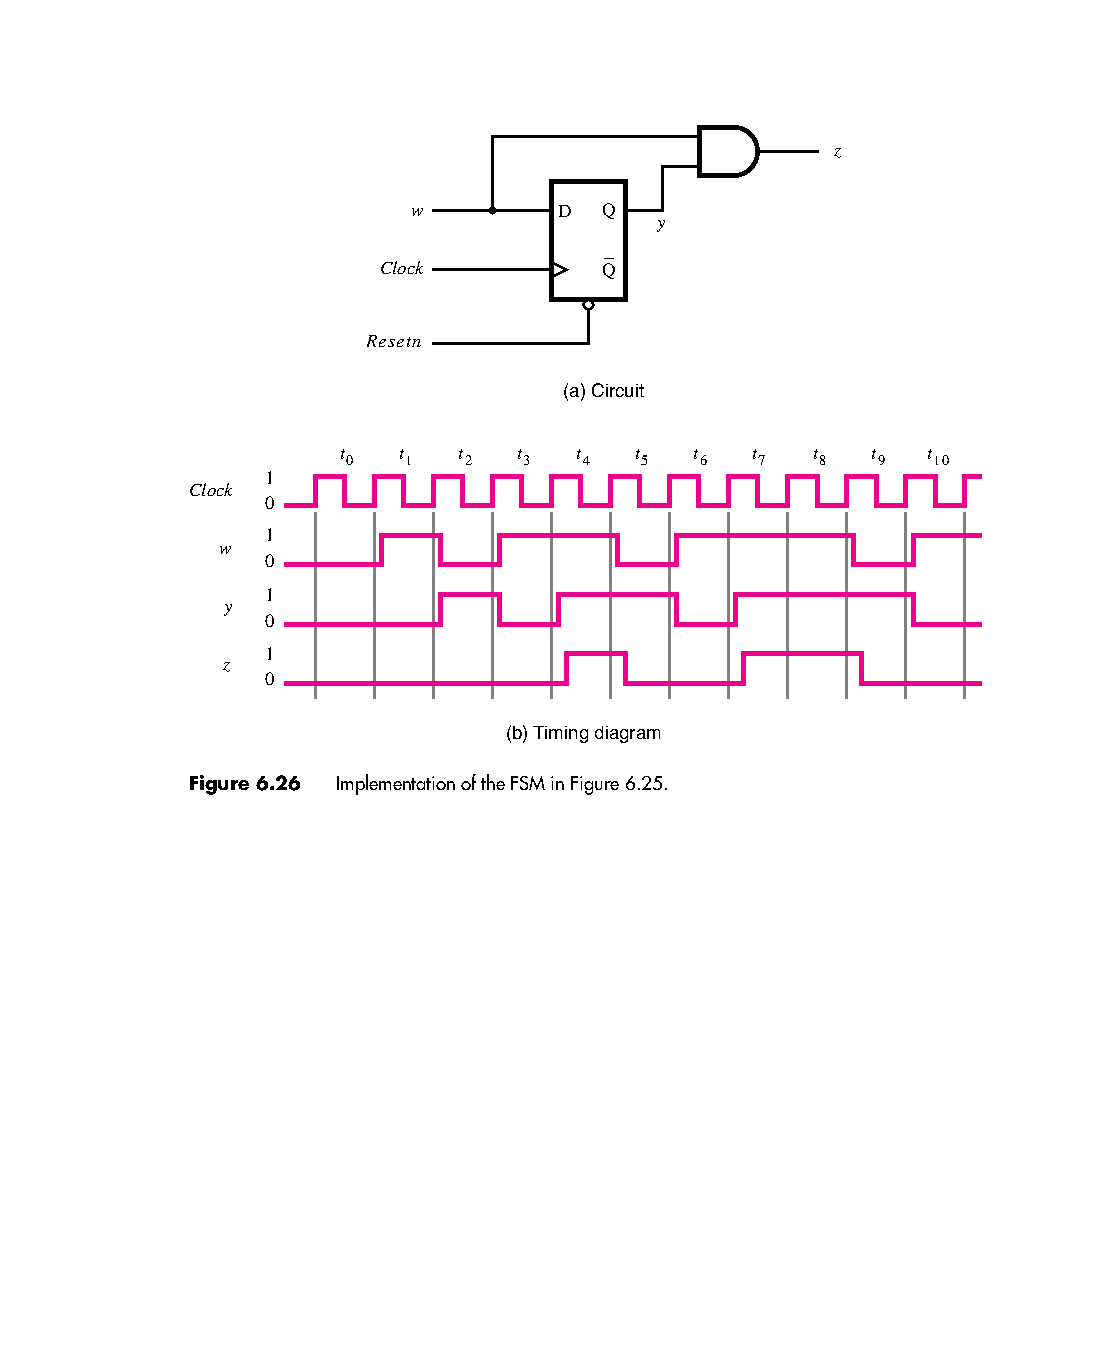
\includegraphics[scale=.7]{figs/VerilogFig6_26}
}

\begin{frame}[fragile]
	\frametitle{Comparador de 4 bits}
	\begin{verilogcode}
module compare (A, B, AeqB, AgtB, AltB); 
  input [3:0] A, B;
  output AeqB, AgtB, AltB;
  reg AeqB, AgtB, AltB;

  always @(A or B) 
  begin
    AeqB = 0; 
    AgtB = 0; 
    AltB = 0; 
    if (A == B)
      AeqB = 1; 
    else if (A > B)
      AgtB = 1;
    else
      AltB = 1;
  end 
  endmodule
    \end{verilogcode} 
\end{frame}

\subsection{Implementação (II)}

\begin{frame}[fragile]
	\frametitle{Usando \texttt{generate}}
	\begin{verilogcode}
module addern (carryin, X, Y, S, carryout); 
  parameter n = 32;
  input carryin;
  input [n-1:0] X, Y;
  output [n-1:0] S; 
  output carryout; 
  wire [n:0] C;

  genvar k;  
  assign C[0] = carryin; 
  assign carryout = C[n]; 
  generate
    for (k = 0; k < n; k = k + 1) 
    begin: fulladd_stage
      wire z1, z2, z3; //wires within full-adder 
      xor (S[k], X[k], Y[k], C[k]);
      and (z1, X[k], Y[k]);
      and (z2, X[k], C[k]);
      and (z3, Y[k], C[k]);
      or (C[k+1], z1, z2, z3); 
    end
  endgenerate 
endmodule
    \end{verilogcode} 
\end{frame}

\begin{frame}[fragile]
	\frametitle{Usando \texttt{task}}
	\begin{verilogcode}
module mux16to1 (W, S16, f); 
  input [0:15] W;
  input [3:0] S16;
  output f;
  reg f;

  always @(W or S16) 
    case (S16[3:2])
      0: mux4to1 (W[ 0: 3], S16[1:0], f); 
      1: mux4to1 (W[ 4: 7], S16[1:0], f); 
      2: mux4to1 (W[ 8:11], S16[1:0], f); 
      3: mux4to1 (W[12:15], S16[1:0], f);
    endcase

//...
    \end{verilogcode} 
\end{frame}

\begin{frame}[fragile]
	\frametitle{Usando \texttt{task}}
	\begin{verilogcode*}{firstnumber=13}
//...

  // Task that specifies a 4-to-1 multiplexer 
  task mux4to1;
    input [0:3] X; 
    input [1:0] S4; 
    output g;
    reg g;

    case (S4)
      0: g = X[0];
      1: g = X[1]; 
      2: g = X[2]; 
      3: g = X[3];
    endcase 
  endtask
endmodule
    \end{verilogcode*} 
\end{frame}

\begin{frame}[fragile]
	\frametitle{Usando \texttt{function}}
	\begin{verilogcode}
module mux16to1 (W, S16, f); 
  input [0:15] W;
  input [3:0] S16;
  output f;
  reg f;
  
  // Function that specifies a 4-to-1 multiplexer 
  function mux4to1;
    input [0:3] X; 
    input [1:0] S4;

    case (S4)
      0: mux4to1 = X[0]; 
      1: mux4to1 = X[1]; 
      2: mux4to1 = X[2]; 
      3: mux4to1 = X[3];
    endcase 
  endfunction
  
//...
    \end{verilogcode} 
\end{frame}

\begin{frame}[fragile]
	\frametitle{Usando \texttt{function}}
	\begin{verilogcode*}{firstnumber=18}
//...
  
  always @(W or S16) 
    case (S16[3:2])
      0: f = mux4to1 (W[ 0: 3], S16[1:0]); 
      1: f = mux4to1 (W[ 4: 7], S16[1:0]); 
      2: f = mux4to1 (W[ 8:11], S16[1:0]); 
      3: f = mux4to1 (W[12:15], S16[1:0]);
    endcase 
endmodule
    \end{verilogcode*} 
\end{frame}

\frame{
    \frametitle{Operadores}
    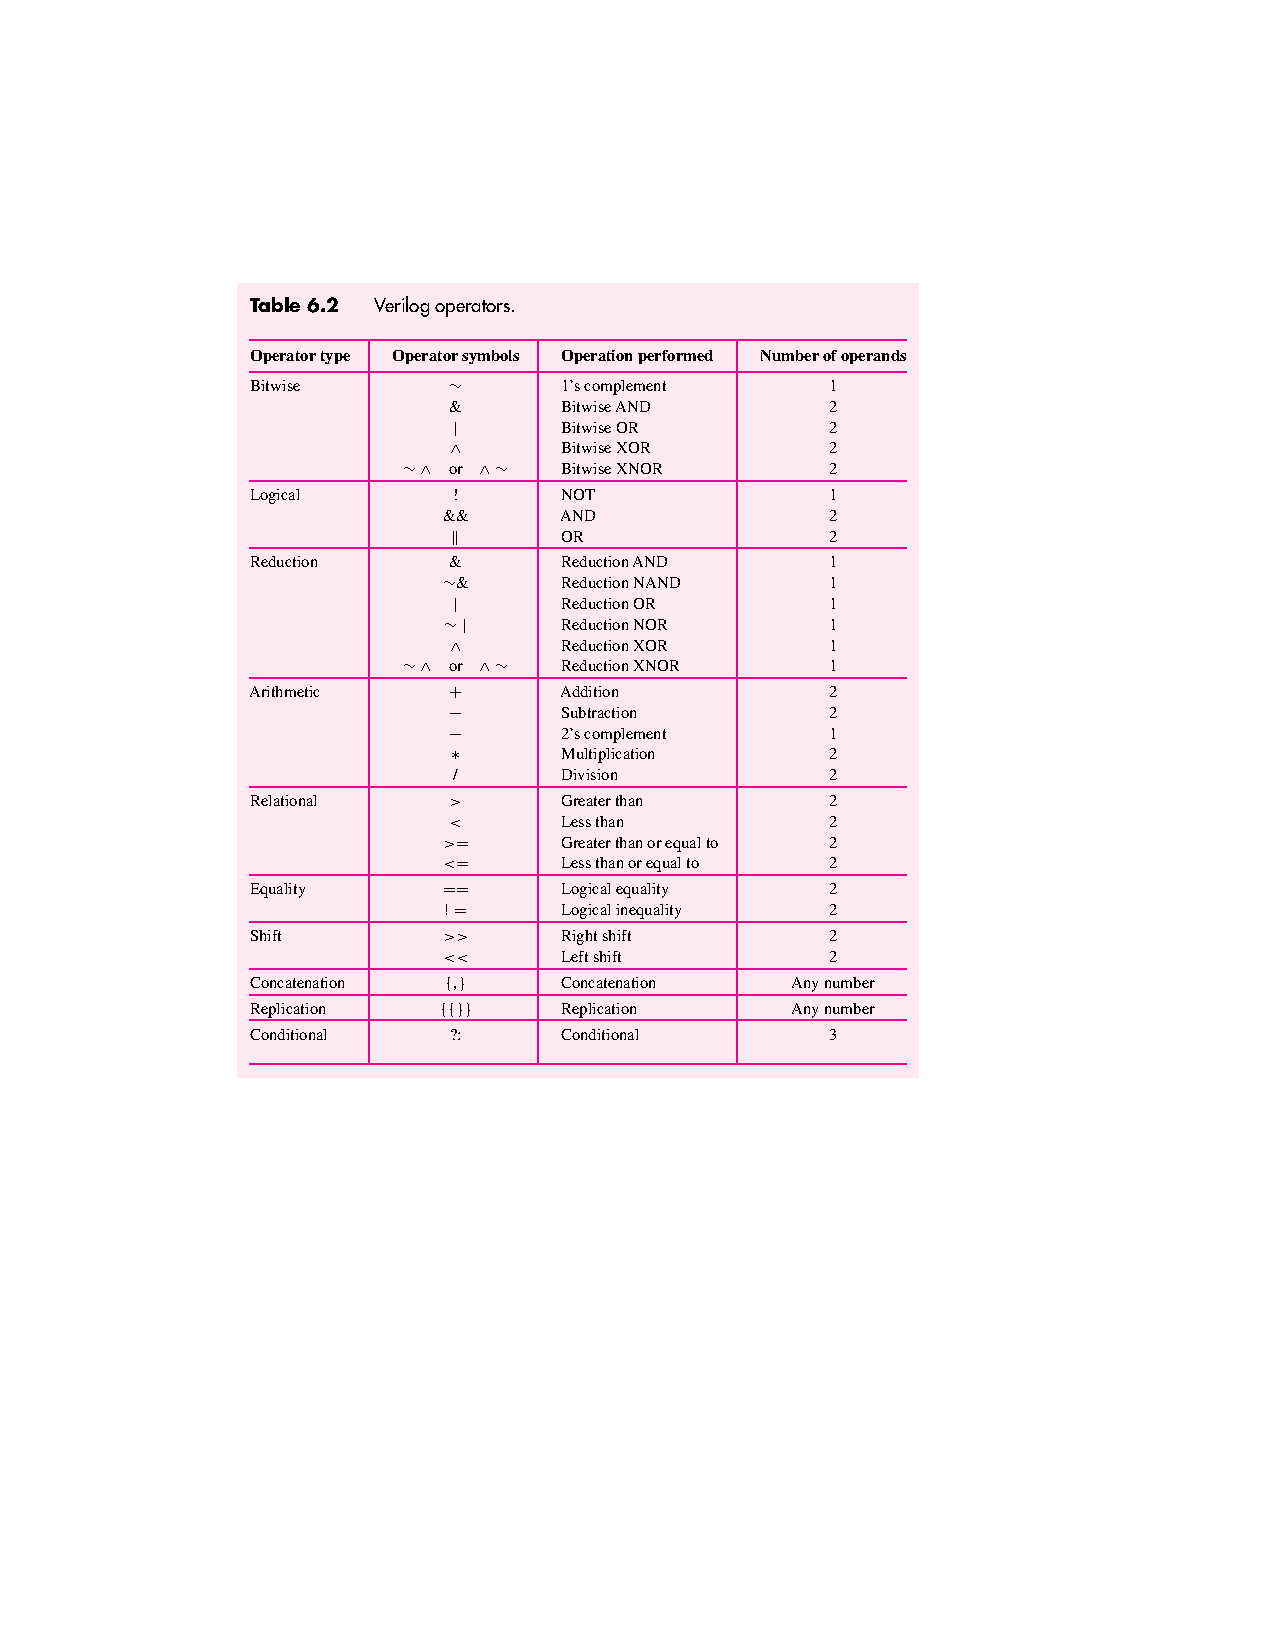
\includegraphics[scale=.6]{figs/VerilogTab6_2}
}

\frame{
    \frametitle{Precedência dos operadores}
    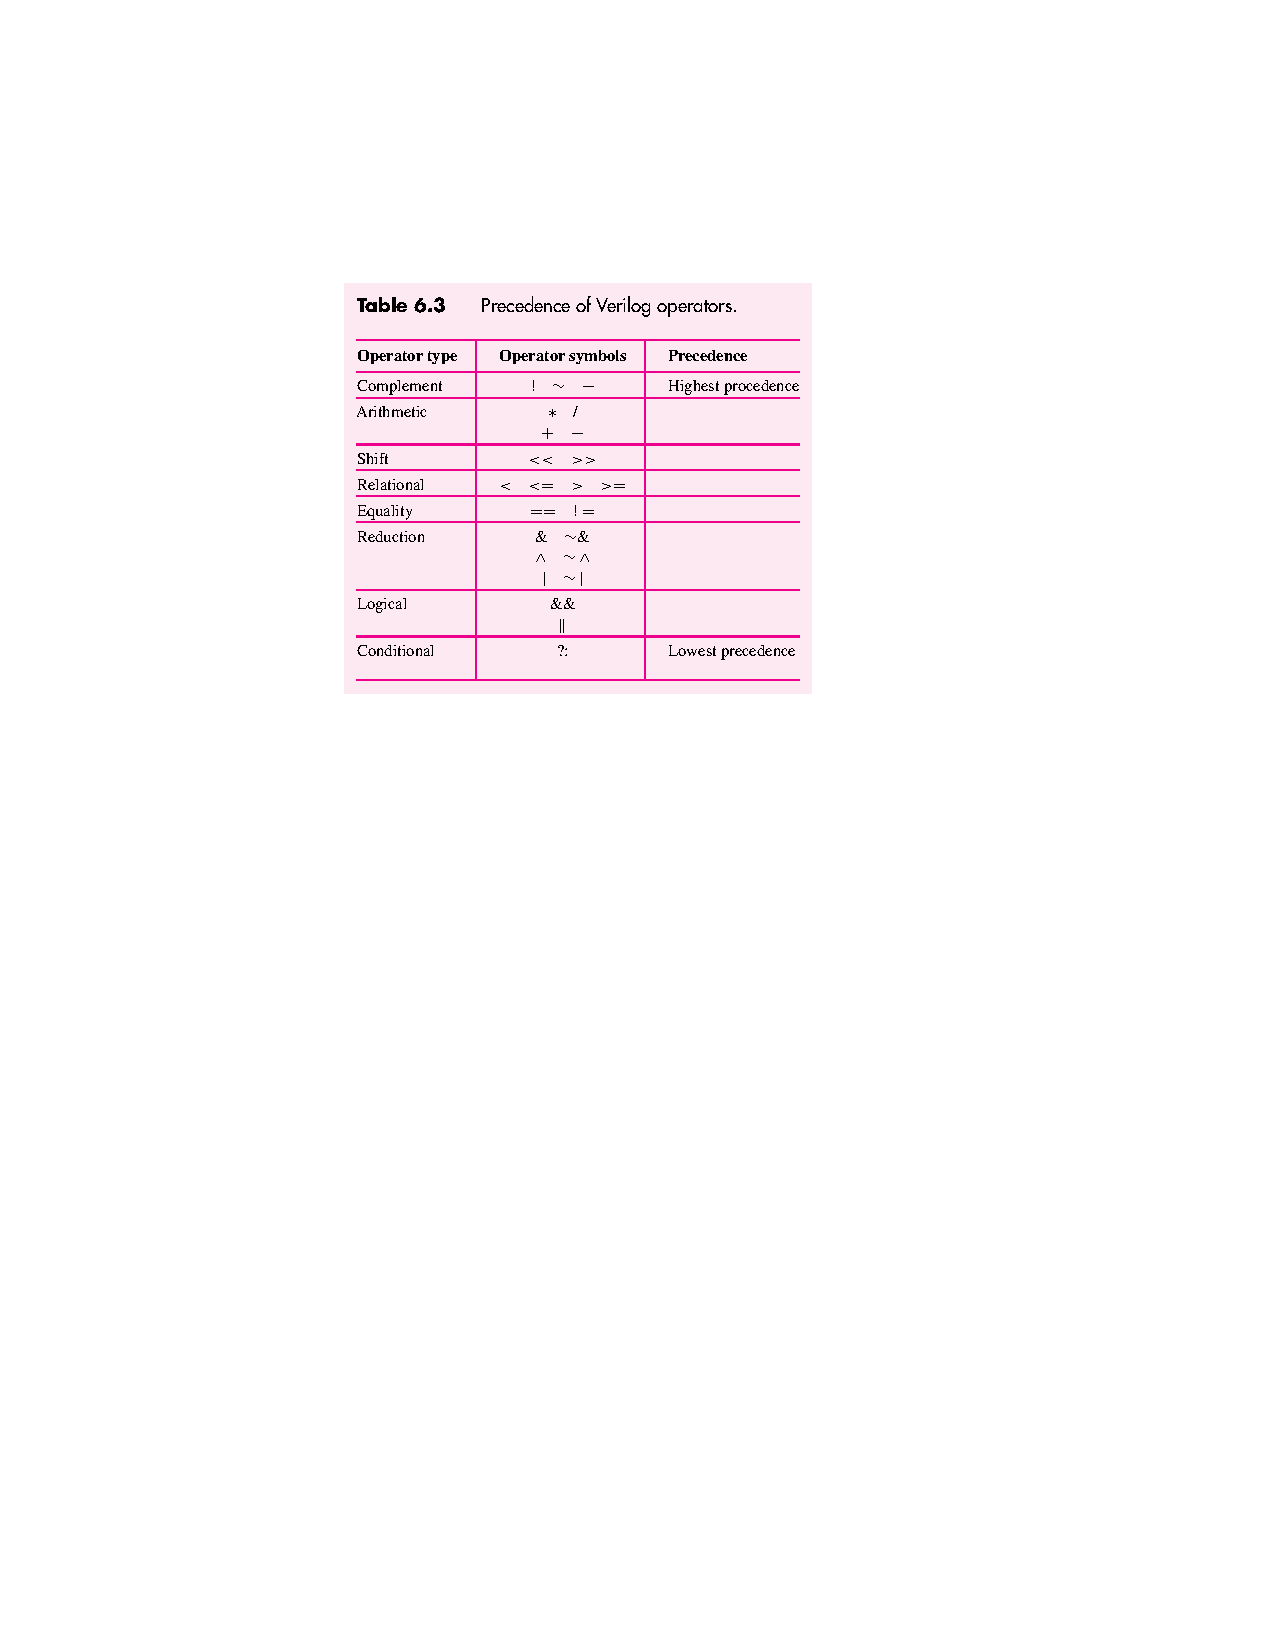
\includegraphics[scale=.7]{figs/VerilogTab6_3}
}

\frame{
    \frametitle{Verilog Registers}
    \begin{itemize}
        \item Nos sistemas digitais, registradores representam elementos de memória (veremos a seguir);
        \item Os registradores digitais precisam de um sinal de relógio (\em{clock}) para operar e atualizar seu estado em determinado nível ou borda; 
        \item Os registradores em Verilog não devem ser confundidos com registradores de hardware;
        \item Em Verilog, o termo register (reg) significa simplesmente um variável que pode conter um valor (equivalente ao signal em VHDL);
        \item Os registradores em Verilog não precisam de um relógio, eles podem ser alterados a qualquer momento, atribuindo-se um novo valor a eles.
    \end{itemize}
}
        
\section{Circuitos Sequenciais}

\subsection{Latchs \& Flip-Flops}

\frame{
    \frametitle{Elementos de memória}
    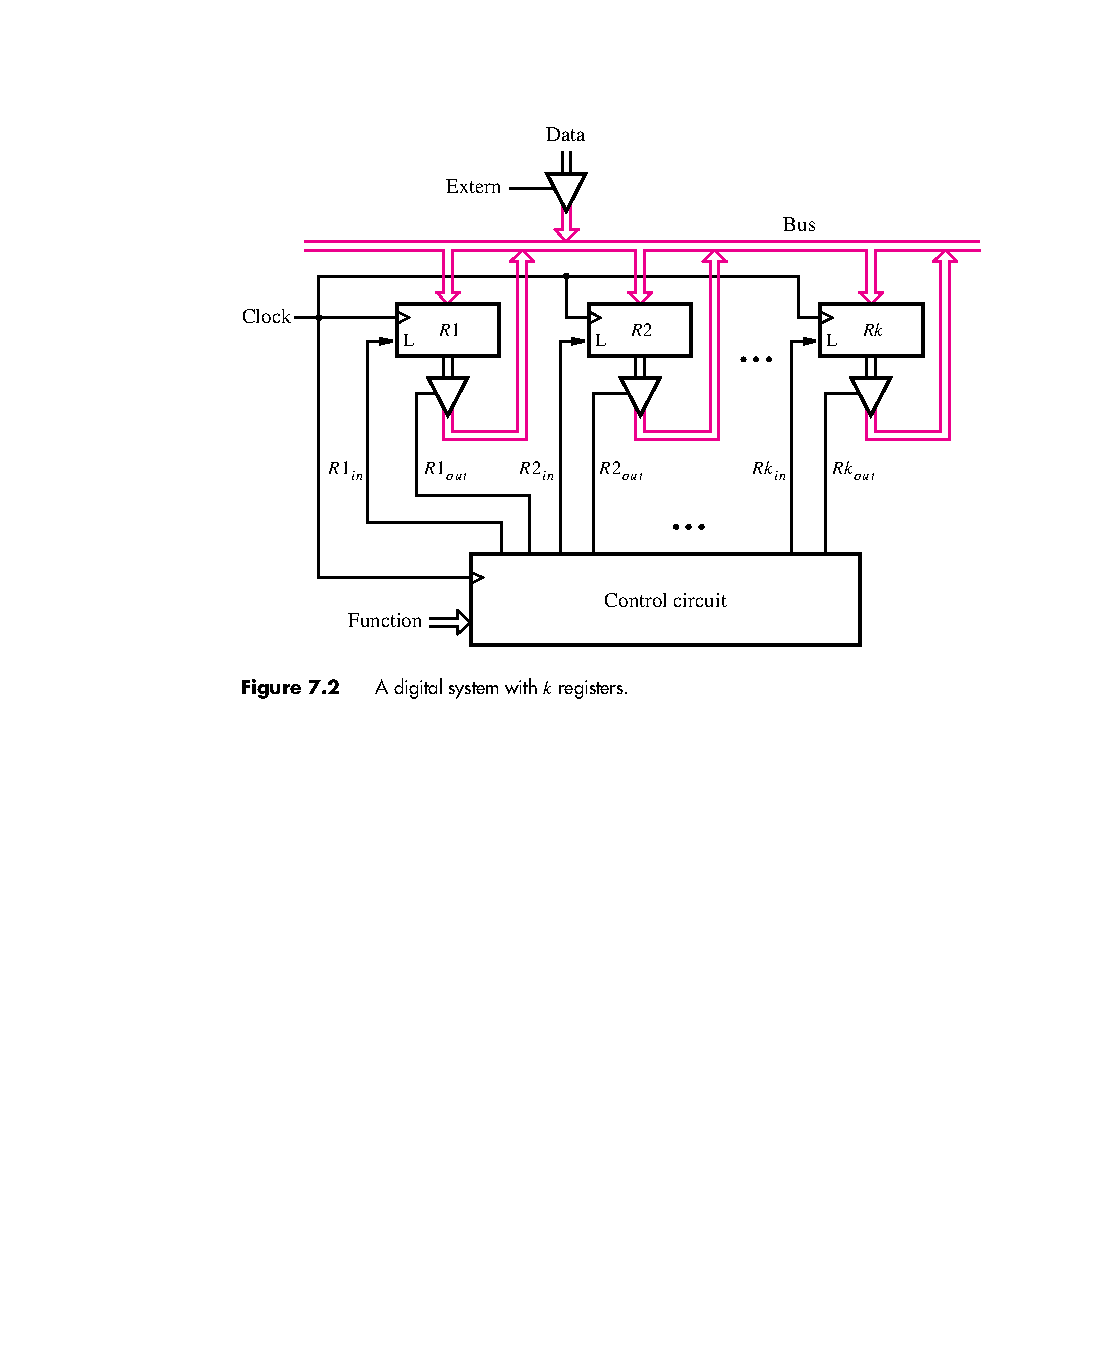
\includegraphics[scale=.7]{figs/VerilogFig7_2}
}

\frame{
    \frametitle{Latch SR}
    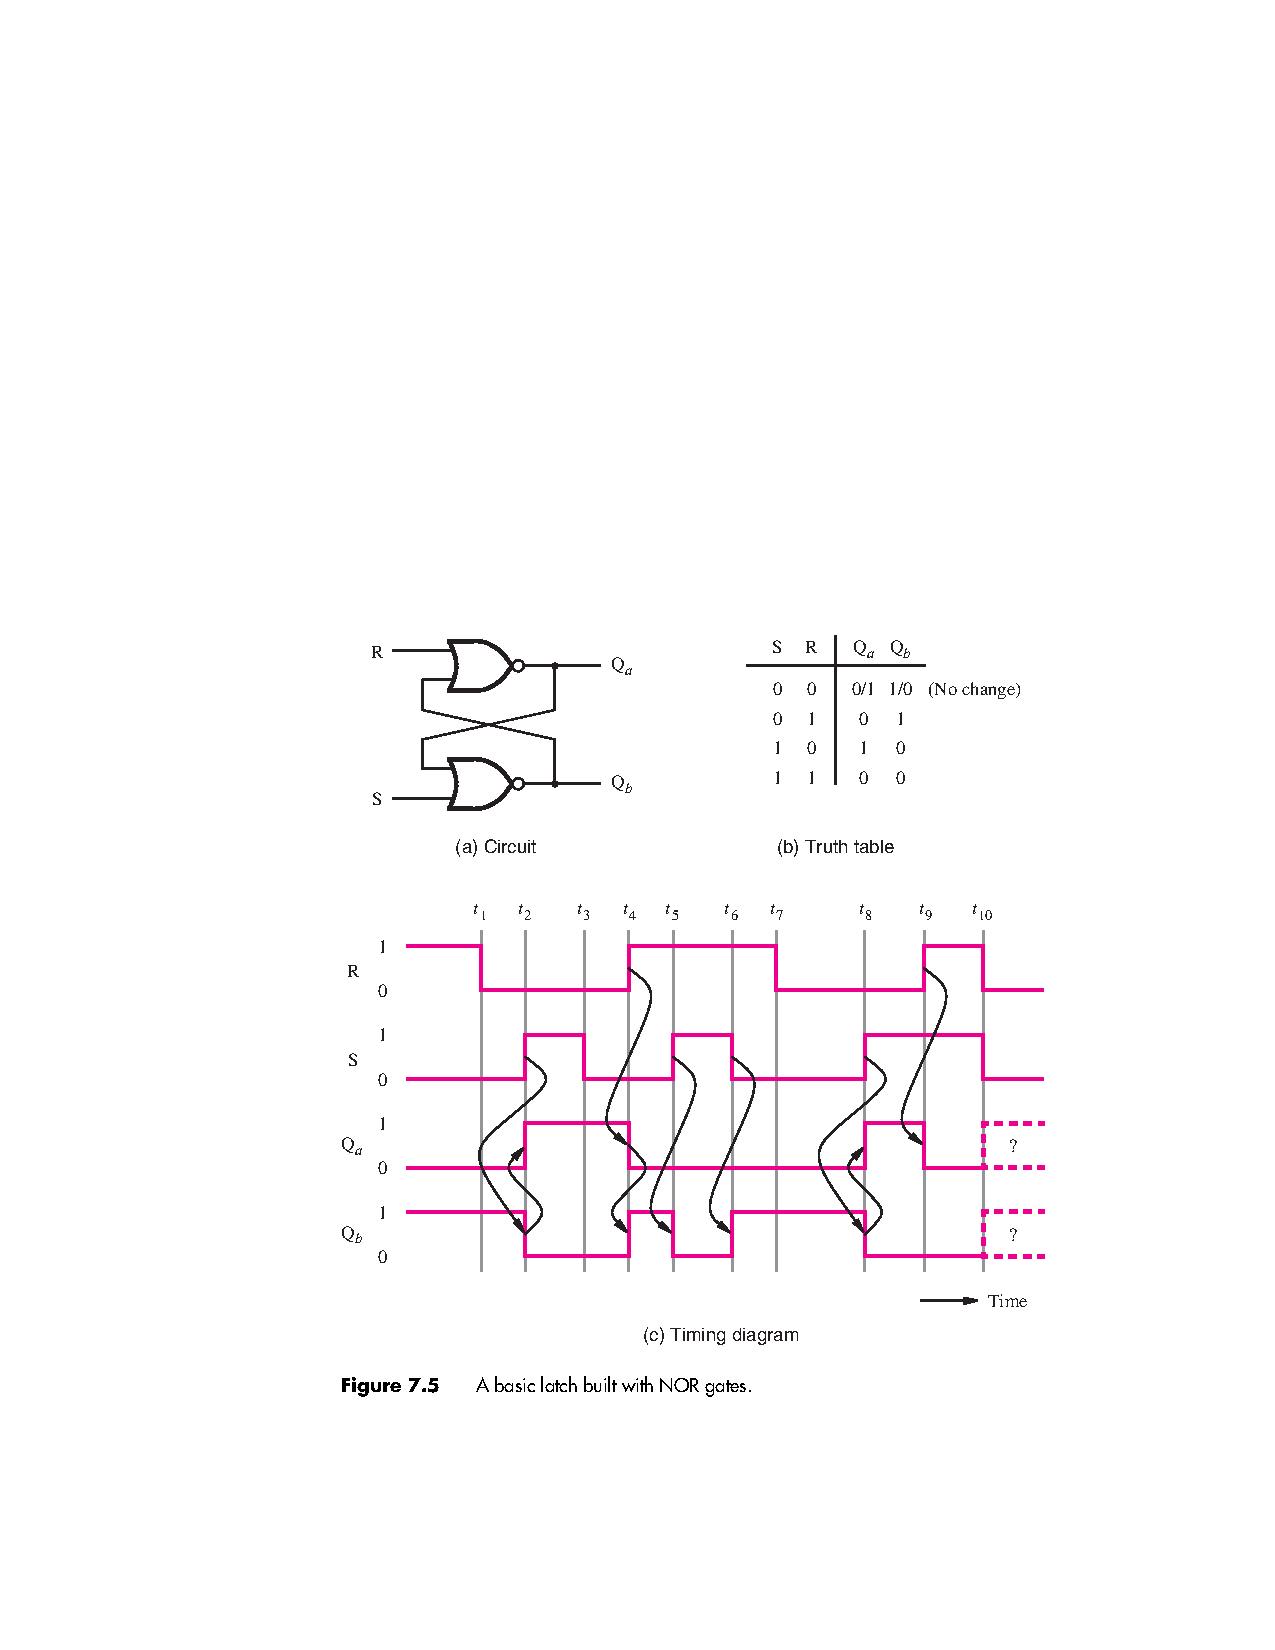
\includegraphics[scale=.6]{figs/VerilogFig7_5}
}

\frame{
    \frametitle{Latch SR com enable}
    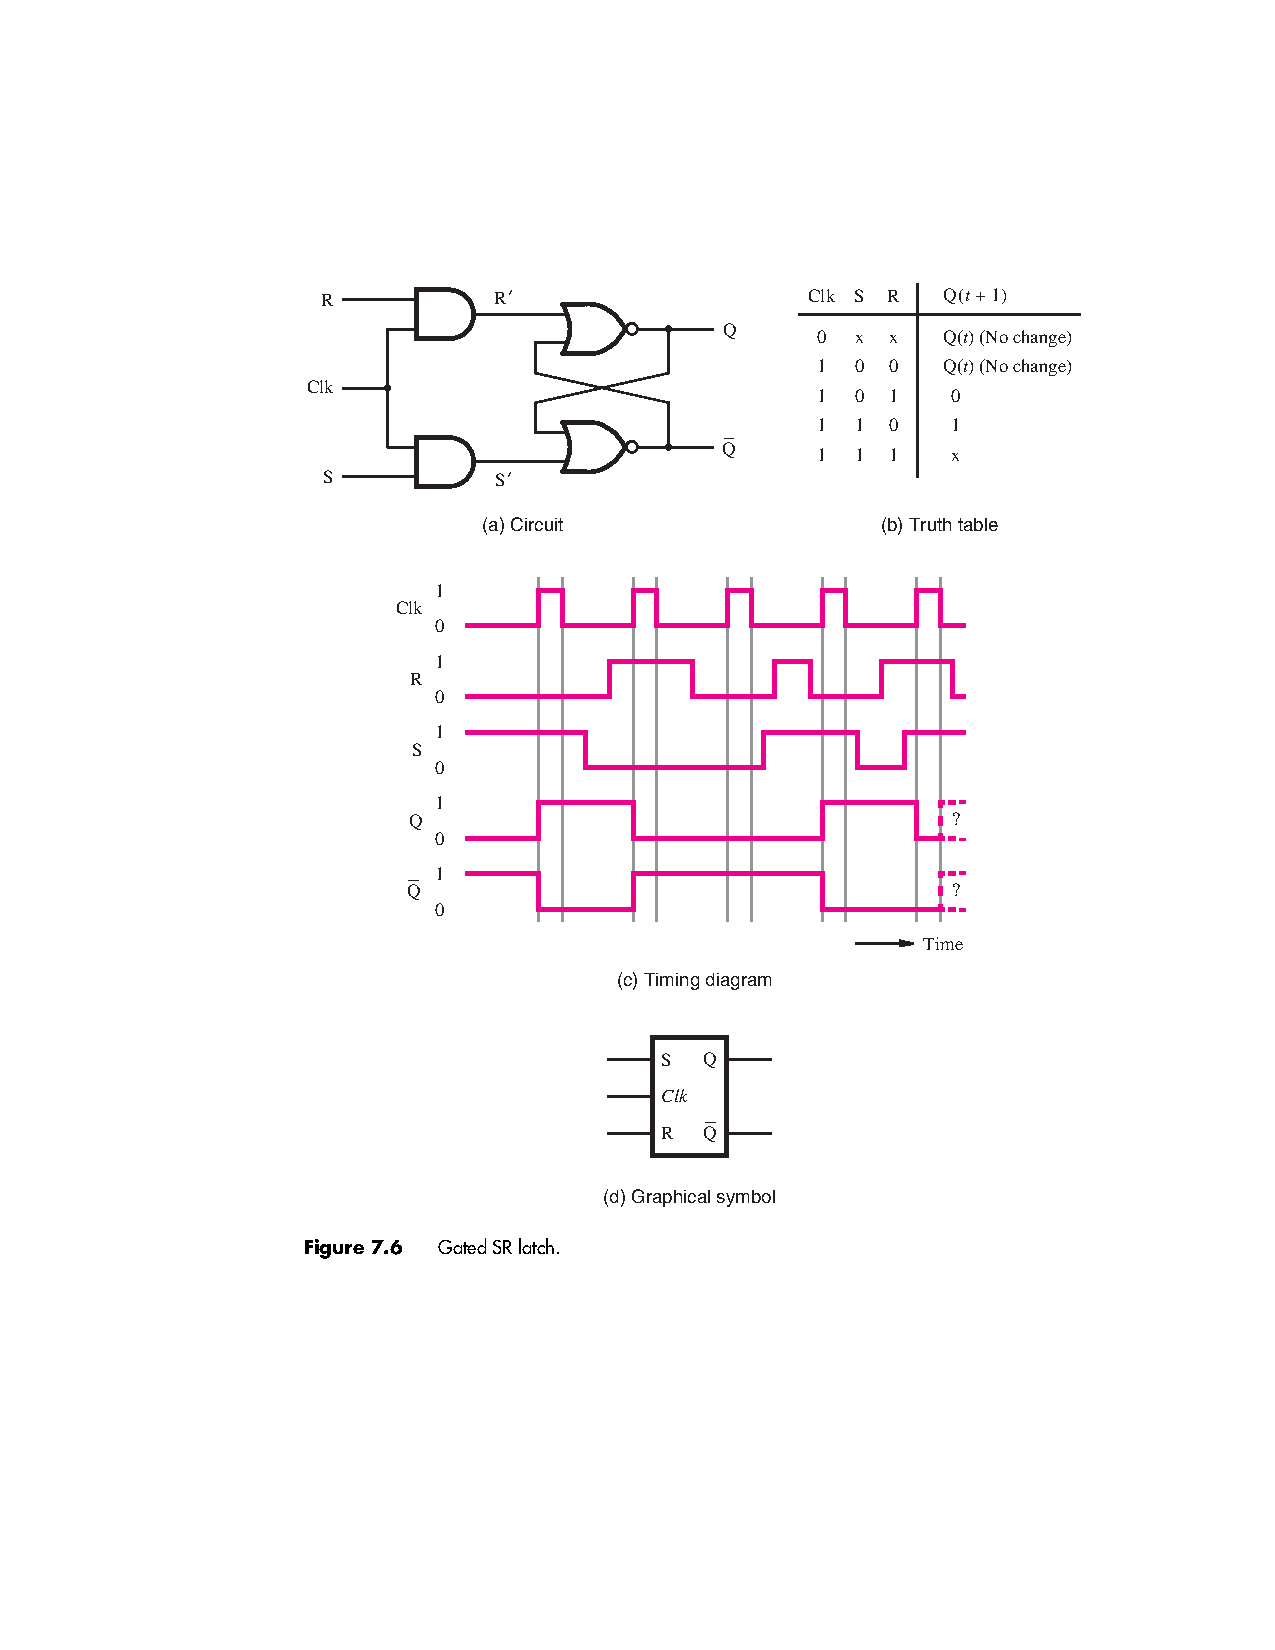
\includegraphics[scale=.5]{figs/VerilogFig7_6}
}

\frame{
    \frametitle{Latch D com enable}
    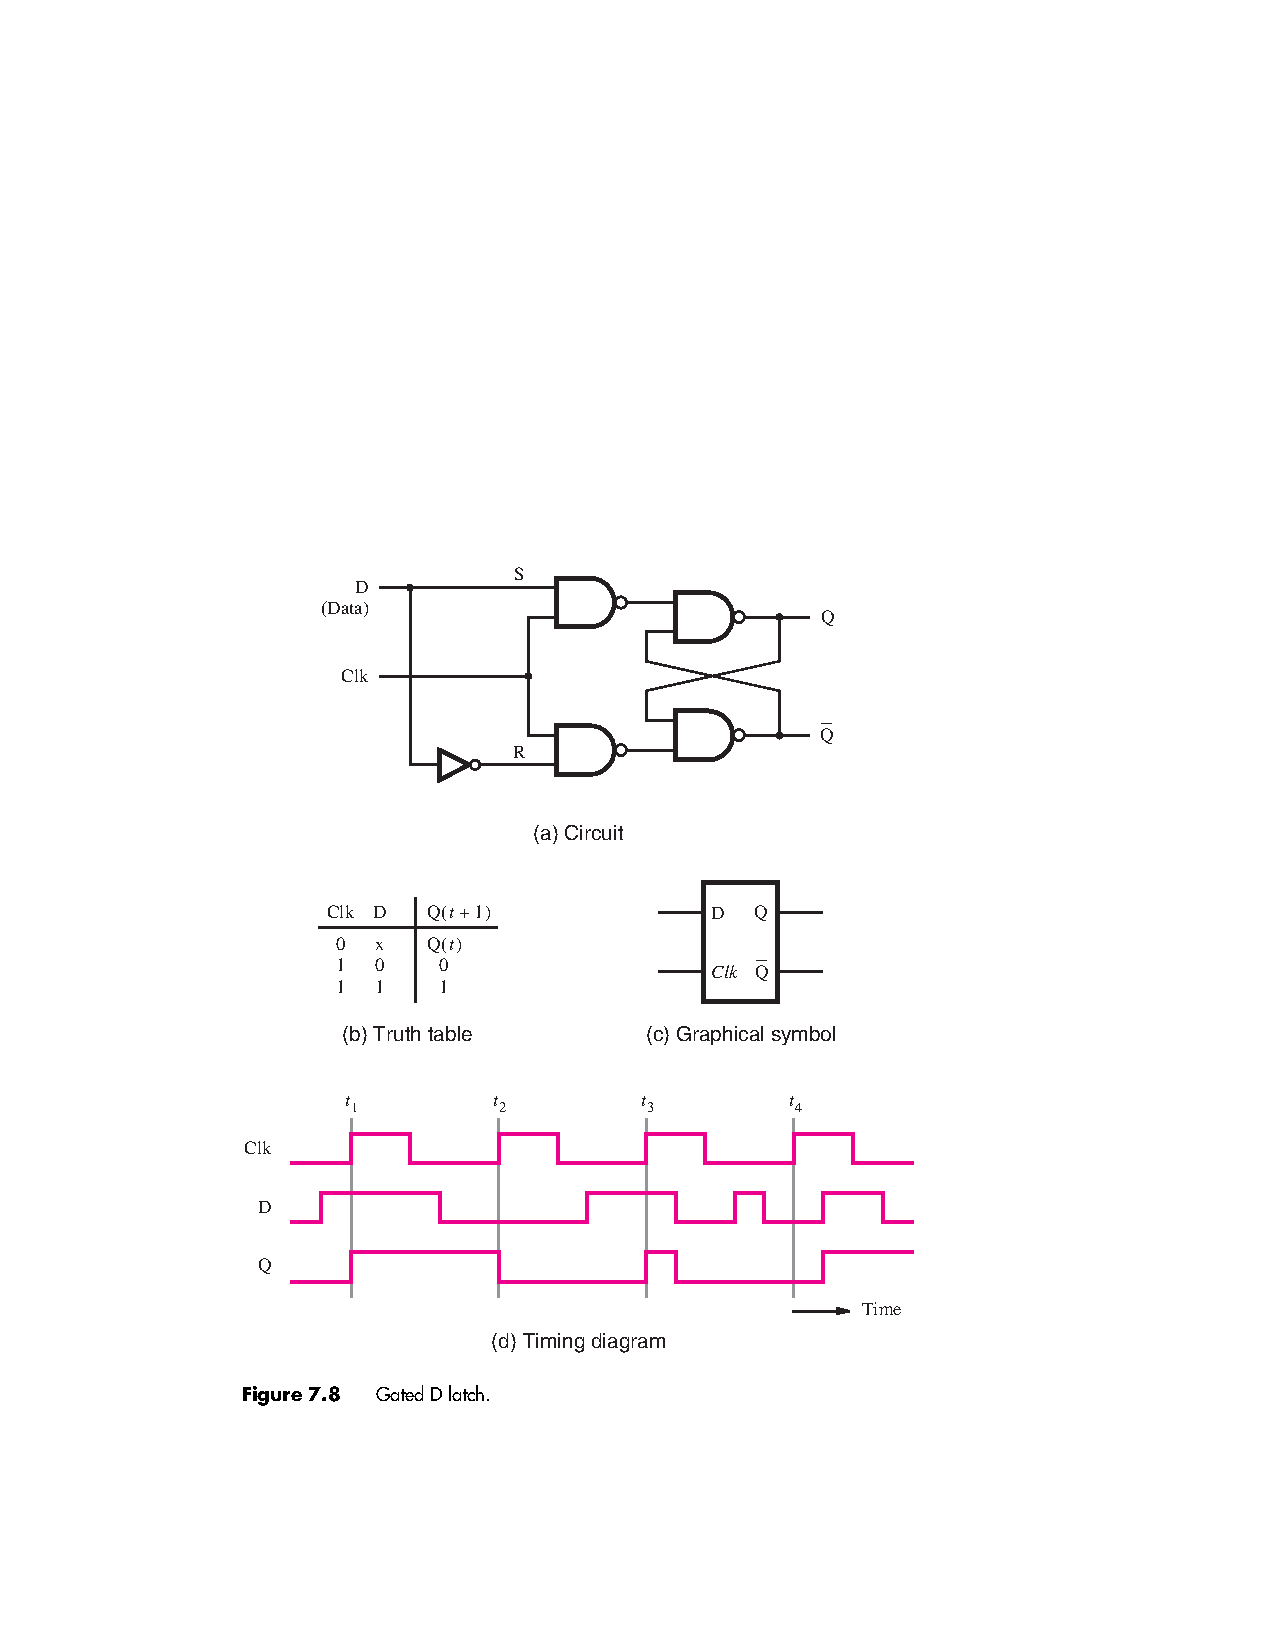
\includegraphics[scale=.6]{figs/VerilogFig7_8}
}

\begin{frame}[fragile]
	\frametitle{Latch D com enable}
	\begin{verilogcode}
module D latch (D, Clk, Q); 
  input D, Clk;
  output Q;
  reg Q;

  always @(D or Clk) 
    if (Clk)
      Q = D;
endmodule
    \end{verilogcode}
\end{frame}

\frame{
    \frametitle{Flip-Flop D Mestre-Escravo}
    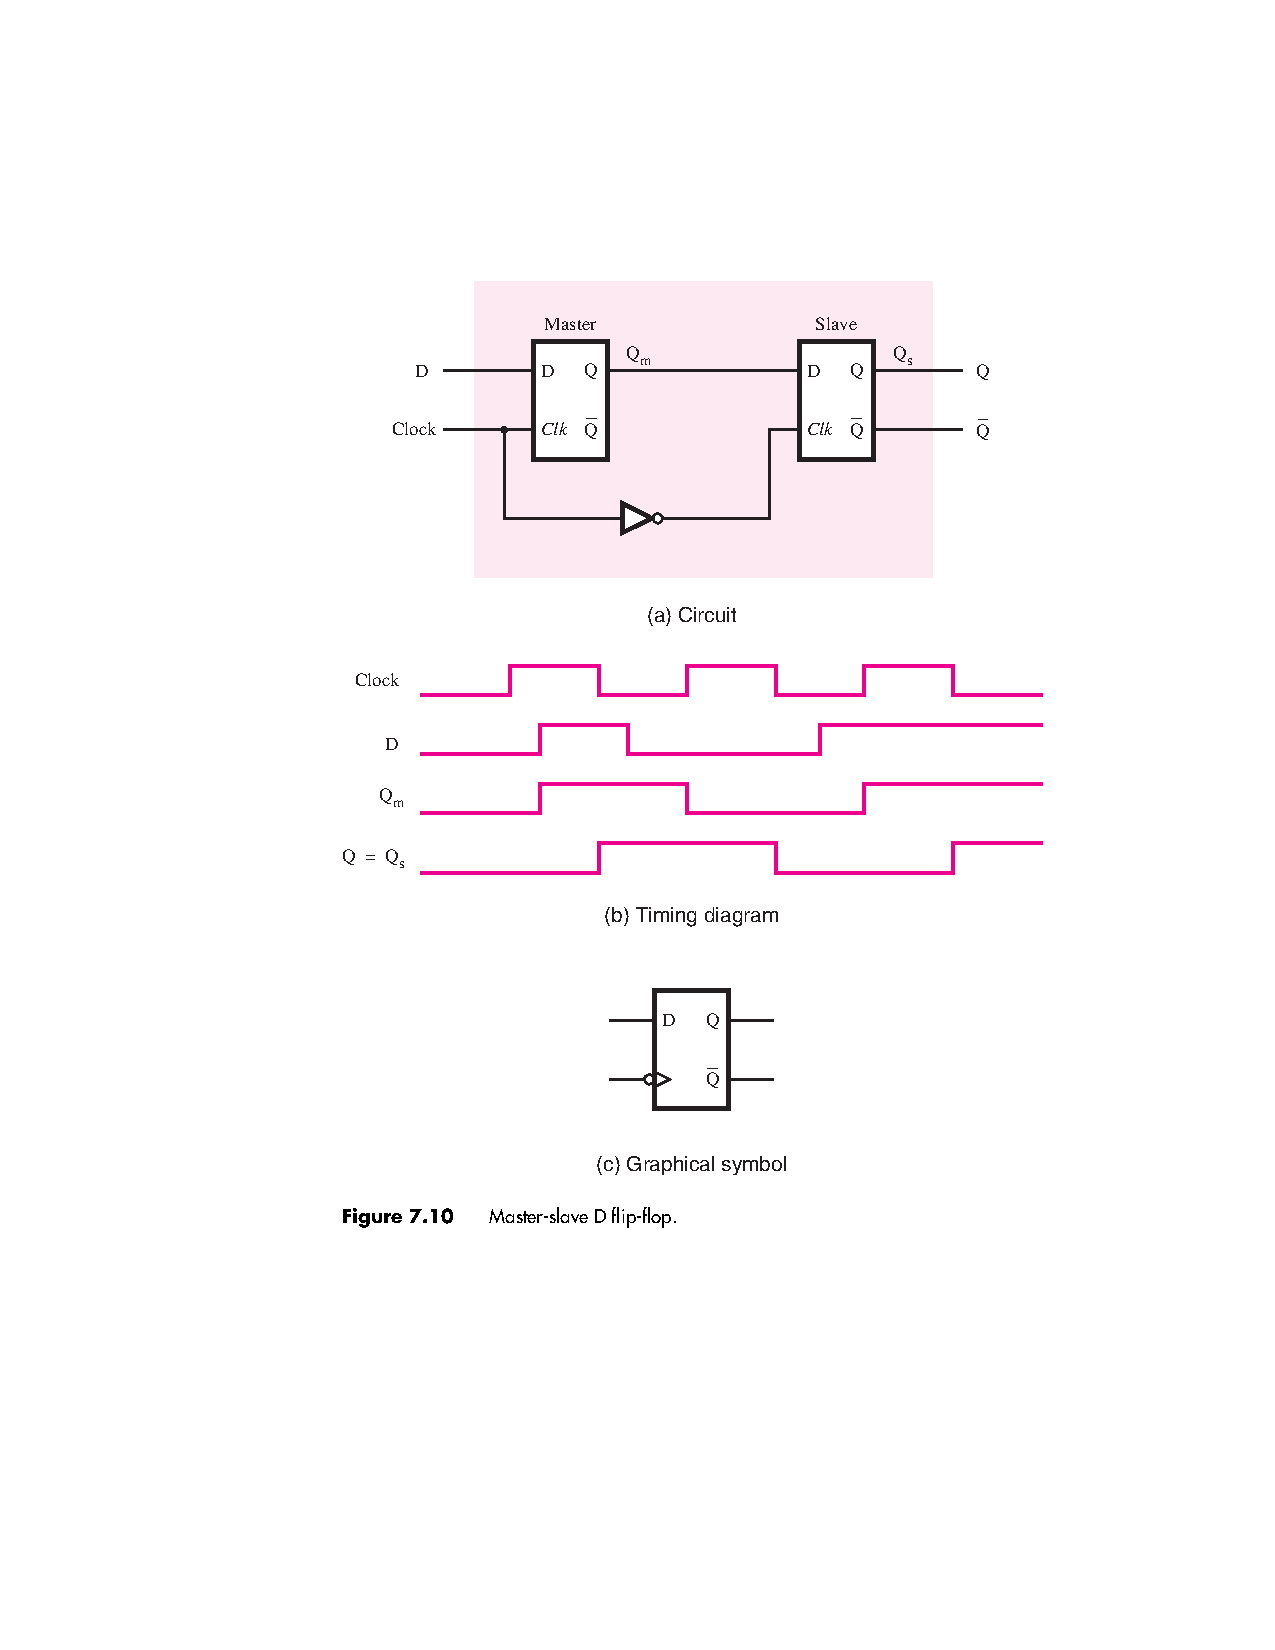
\includegraphics[scale=.5]{figs/VerilogFig7_10}
}

\frame{
    \frametitle{Flip-Flop D Sensível à borda}
    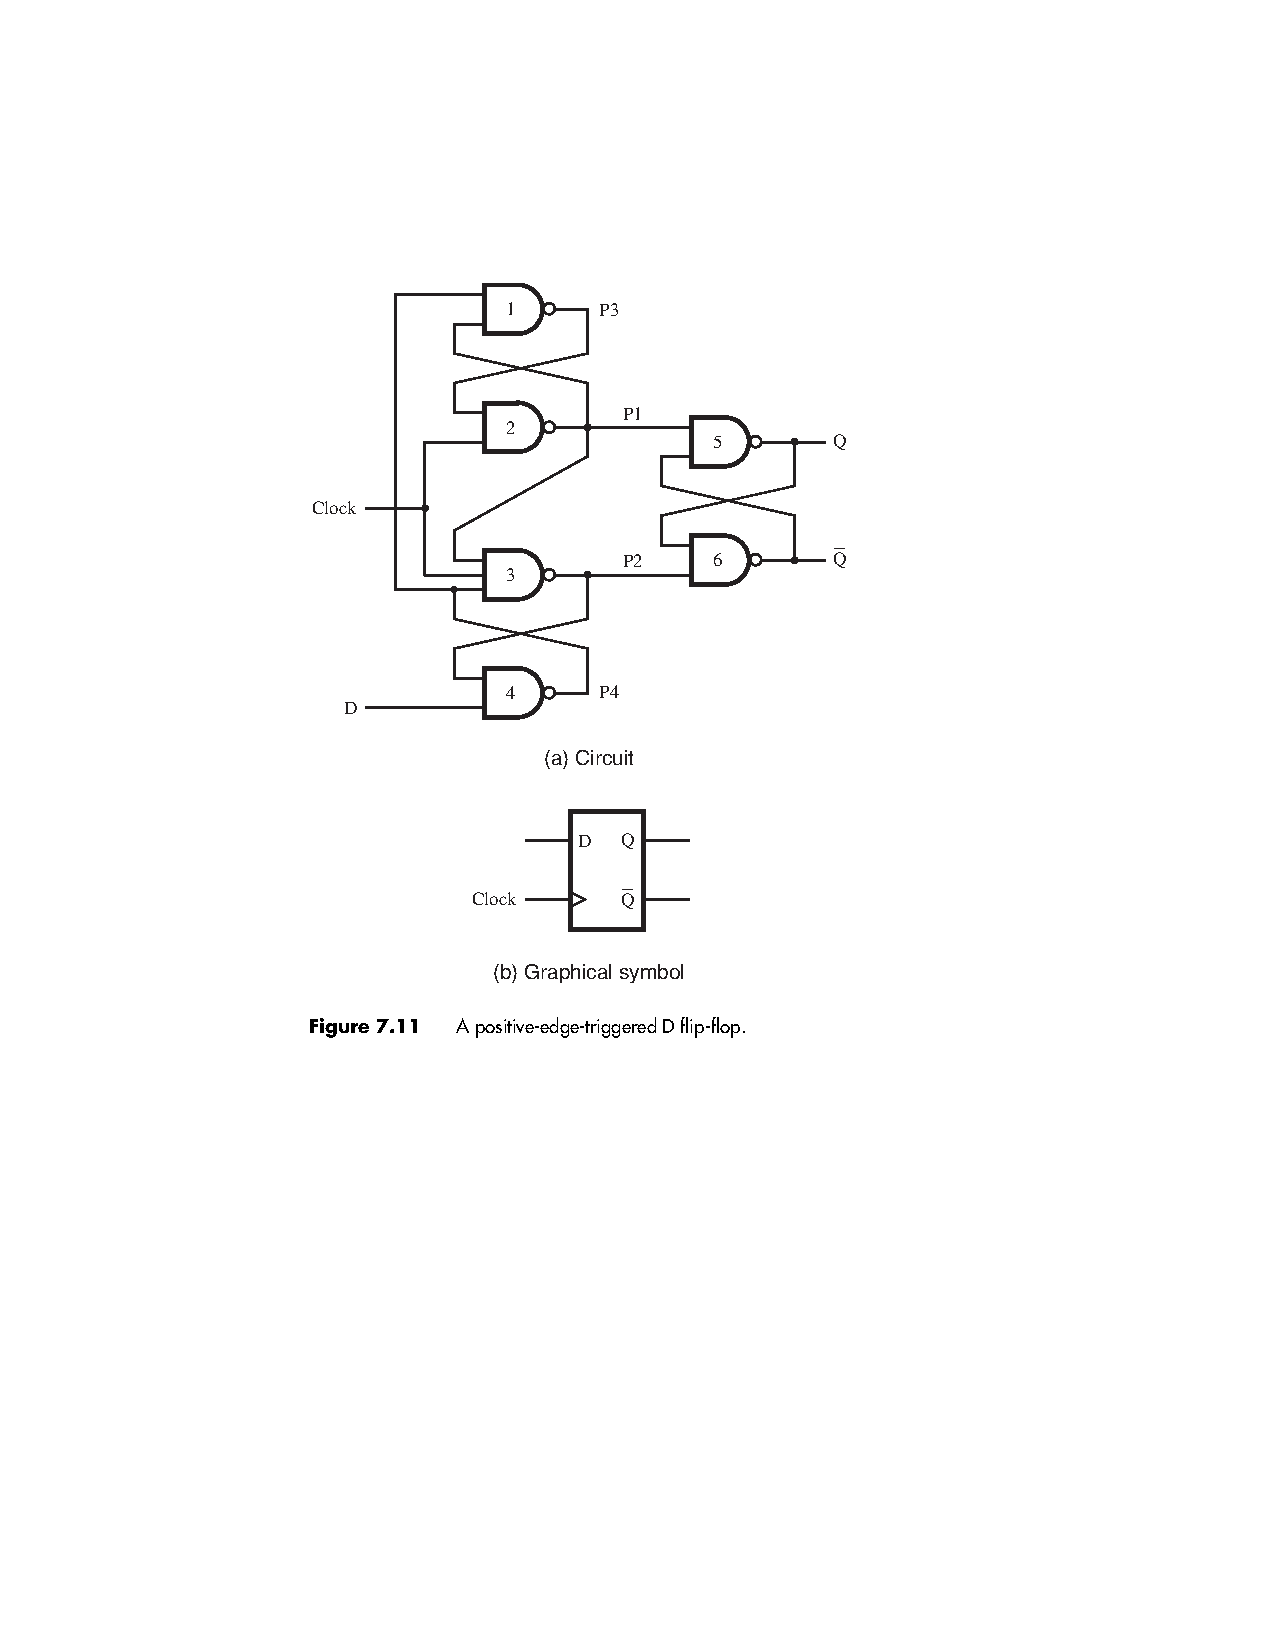
\includegraphics[scale=.6]{figs/VerilogFig7_11}
}

\begin{frame}[fragile]
	\frametitle{}
	\begin{verilogcode}
module flipflop(D, Clock, Q); 
  input D, Clock;
  output Q;
  reg Q;

  always @(posedge Clock) 
    Q = D;
endmodule
    \end{verilogcode}
\end{frame}

\frame{
    \frametitle{Comparação entre nível e borda}
    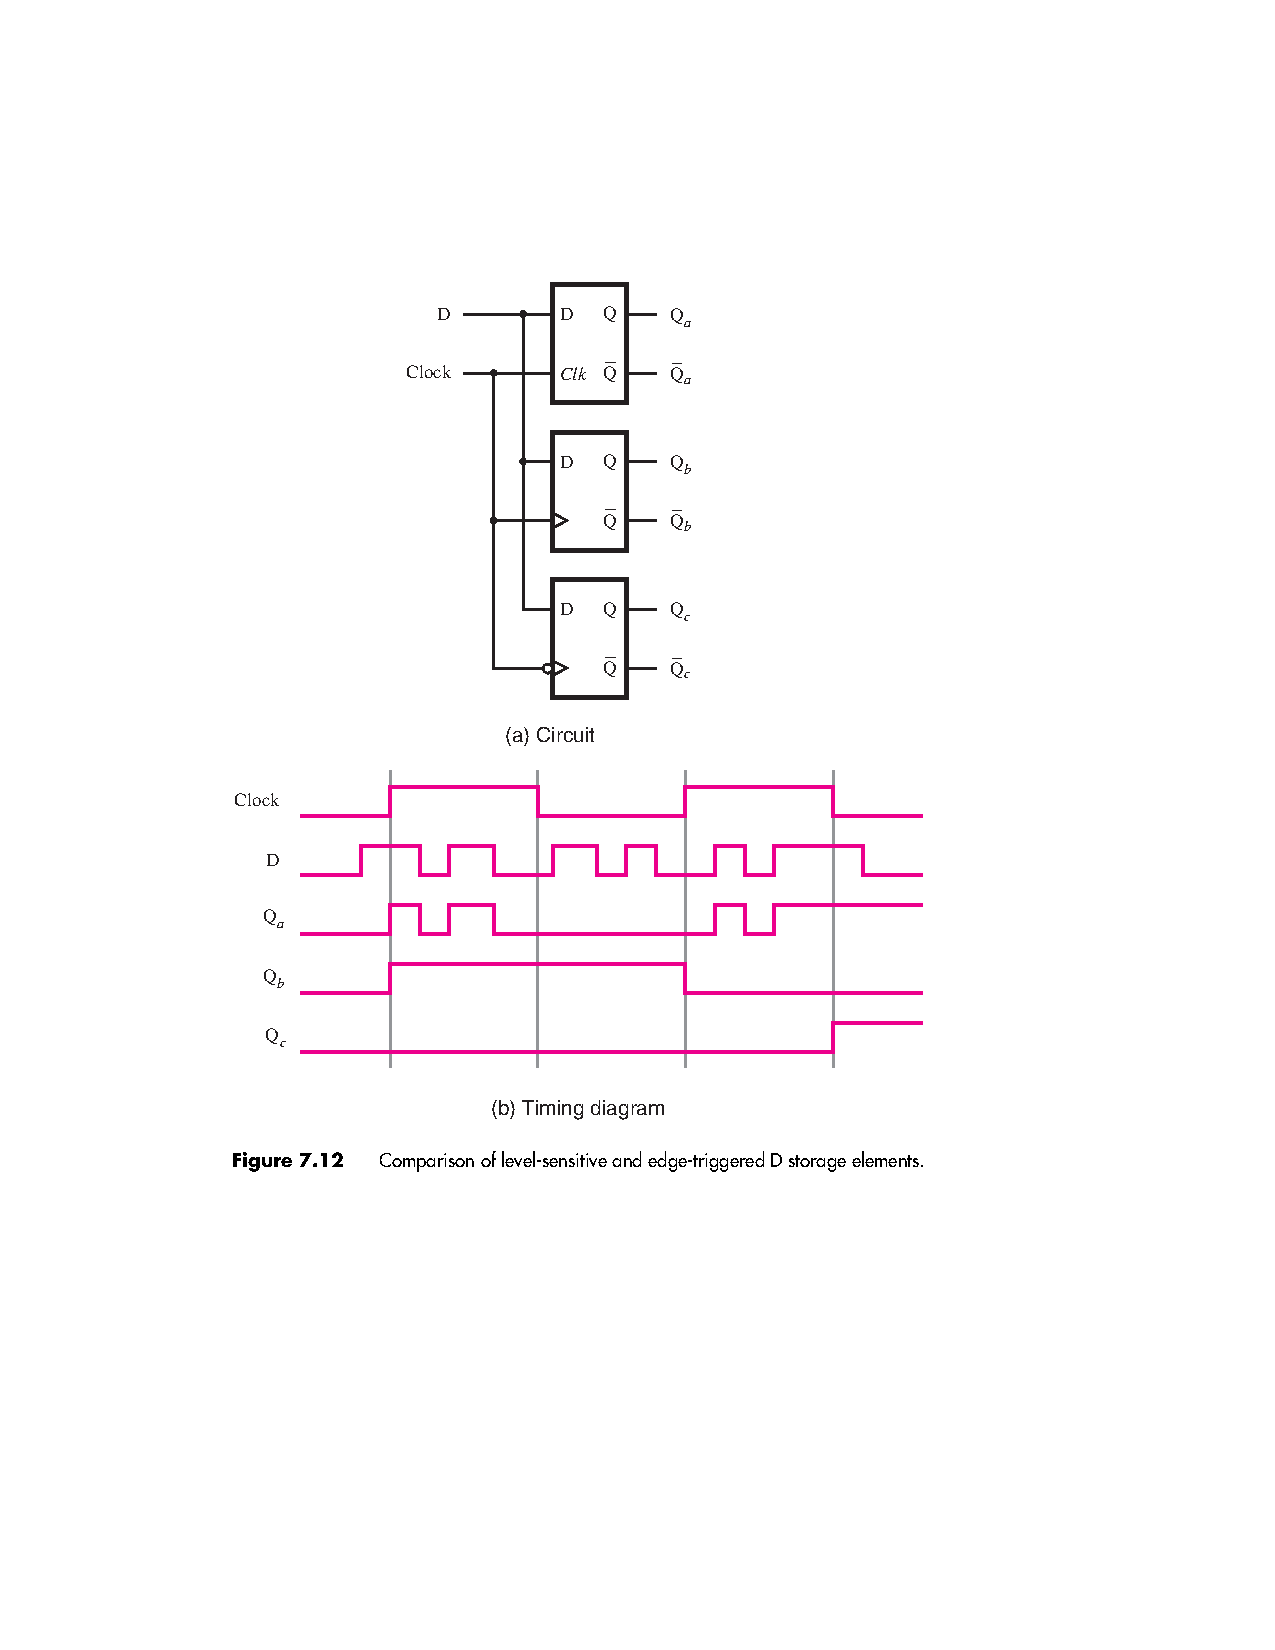
\includegraphics[scale=.55]{figs/VerilogFig7_12}
}

\begin{frame}[fragile]
	\frametitle{Blocking}
	\begin{verilogcode}
module example7_3 (D, Clock, Q1, Q2); 
  input D, Clock;
  output Q1, Q2;
  reg Q1, Q2;

  always @(posedge Clock) 
  begin
    Q1 = D;
    Q2 = Q1;
  end 
endmodule
    \end{verilogcode}
    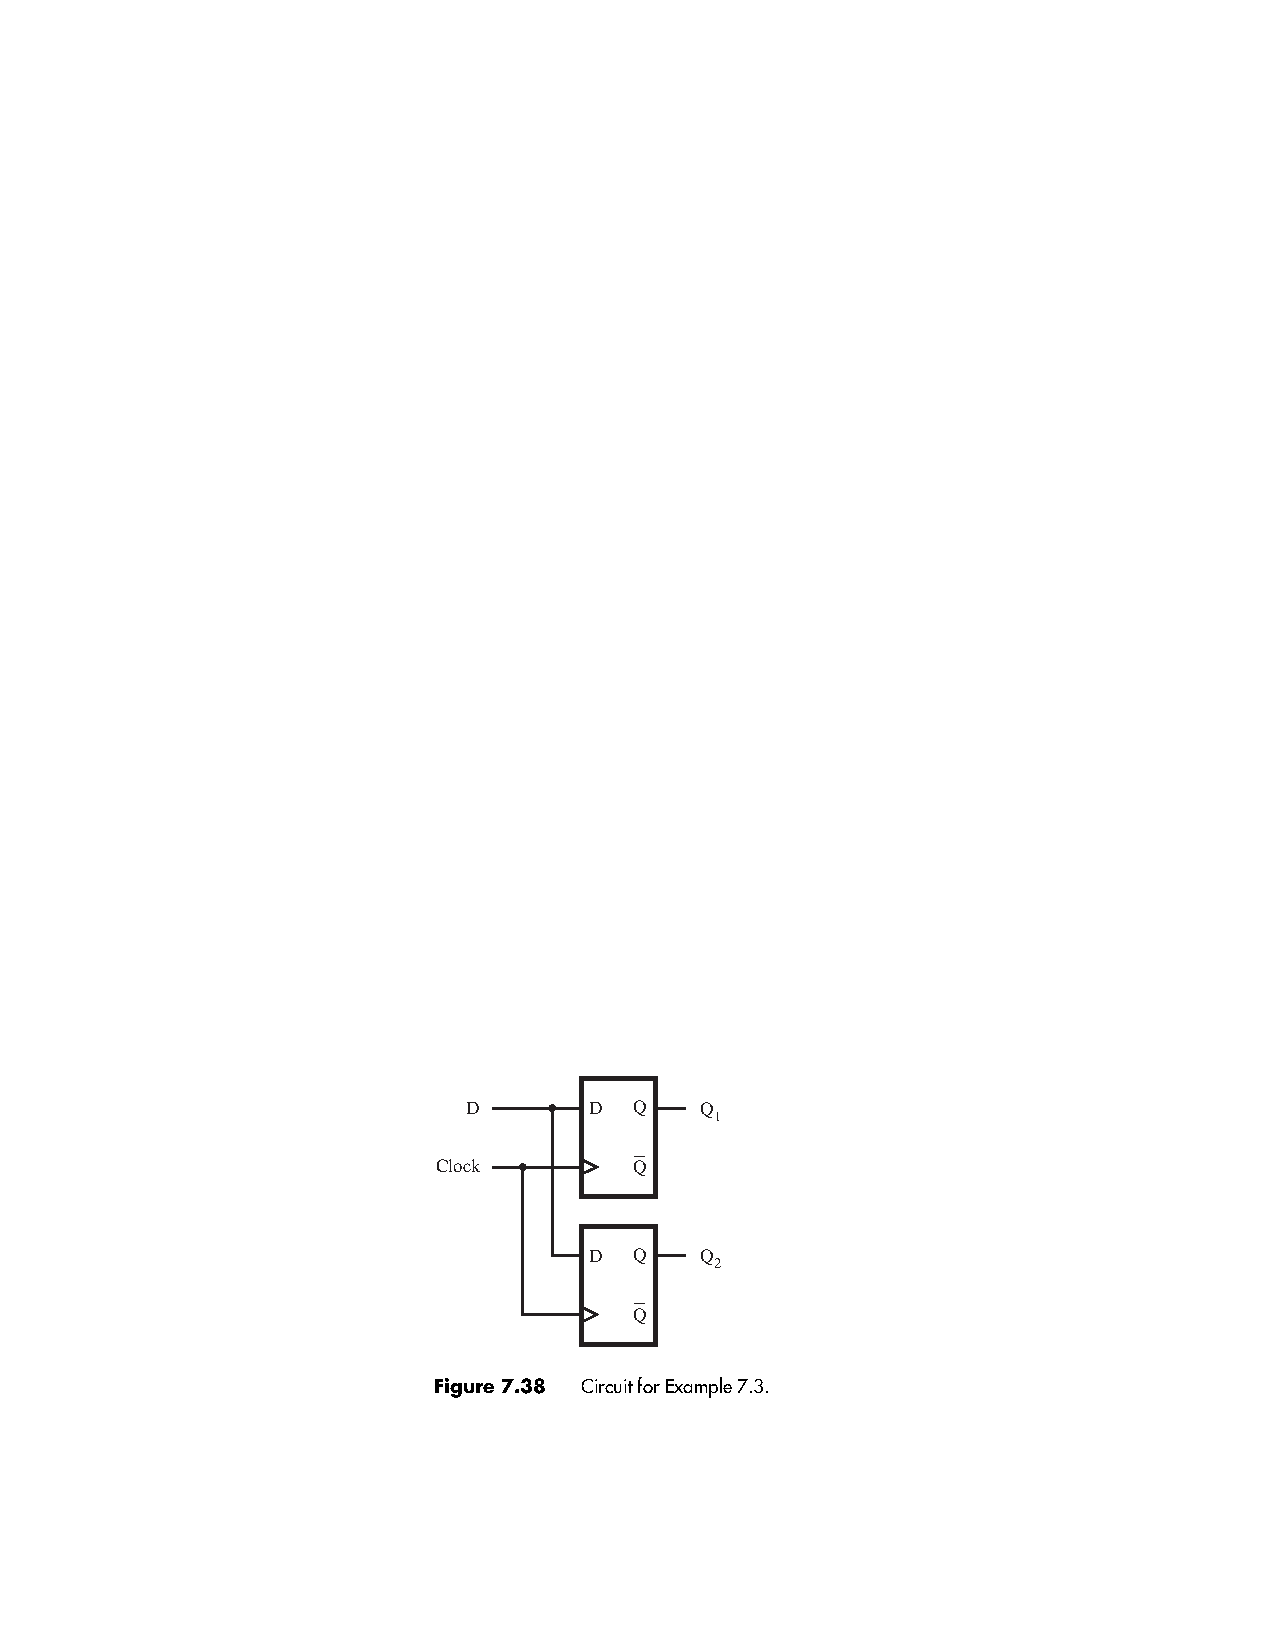
\includegraphics[scale=.7]{figs/VerilogFig7_38}
\end{frame}


\begin{frame}[fragile]
	\frametitle{Non-Blocking}
	\begin{verilogcode}
module example7_4 (D, Clock, Q1, Q2); 
  input D, Clock;
  output Q1, Q2;
  reg Q1, Q2;

  always @(posedge Clock) 
  begin
    Q1 <= D;
    Q2 <= Q1; 
  end
endmodule
	\end{verilogcode}
    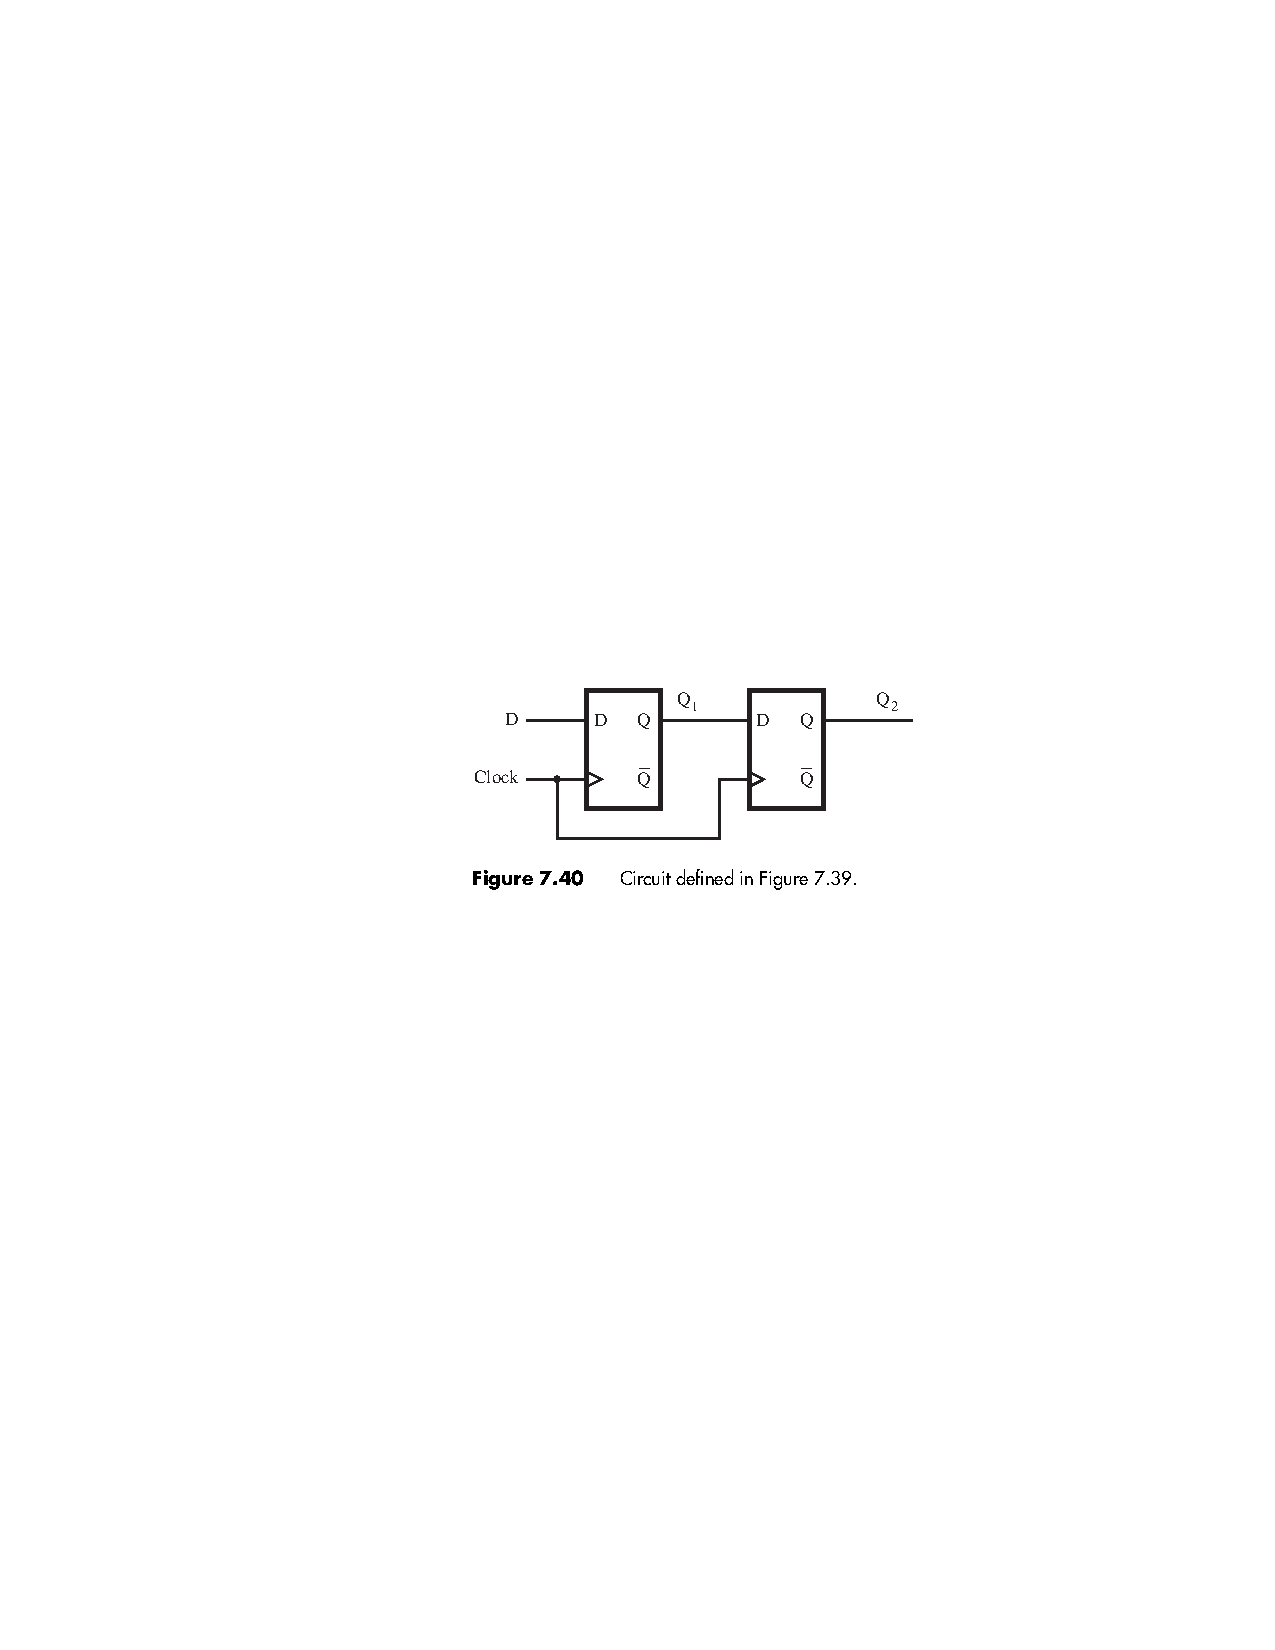
\includegraphics[scale=.7]{figs/VerilogFig7_40}
\end{frame}

\begin{frame}[fragile]
	\frametitle{Blocking}
	\begin{verilogcode}
module example7_5 (x1, x2, x3, Clock, f, g); 
  input x1, x2, x3, Clock;
  output f, g;
  reg f, g;

  always @(posedge Clock) 
  begin
    f = x1 & x2; 
    g = f | x3; // ordem importa!
  end
endmodule
    \end{verilogcode}
    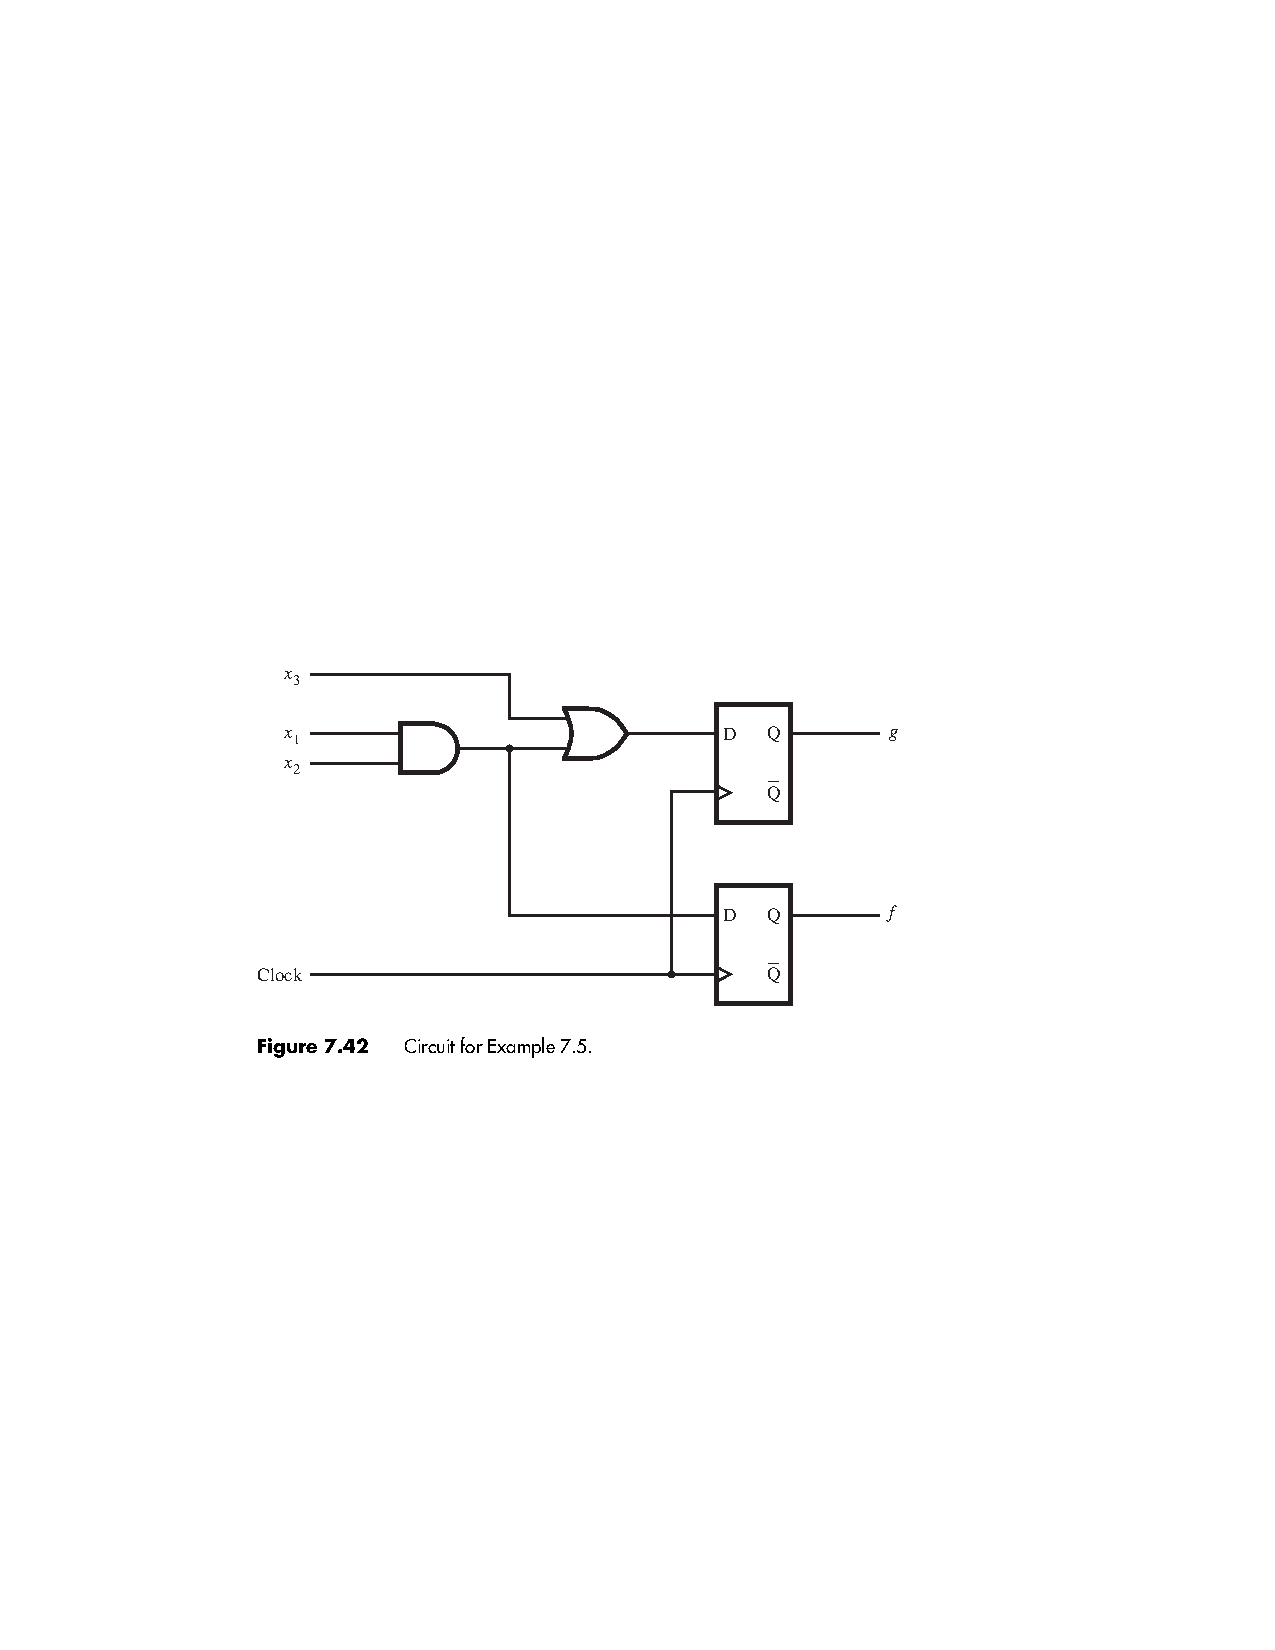
\includegraphics[scale=.6]{figs/VerilogFig7_42}
\end{frame}


\begin{frame}[fragile]
	\frametitle{Non-Blocking}
	\begin{verilogcode}
module example7_6 (x1, x2, x3, Clock, f, g); 
  input x1, x2, x3, Clock;
  output f, g;
  reg f, g;

  always @(posedge Clock) 
  begin
    f <= x1 & x2;
    g <= f | x3; 
  end
endmodule
	\end{verilogcode}
    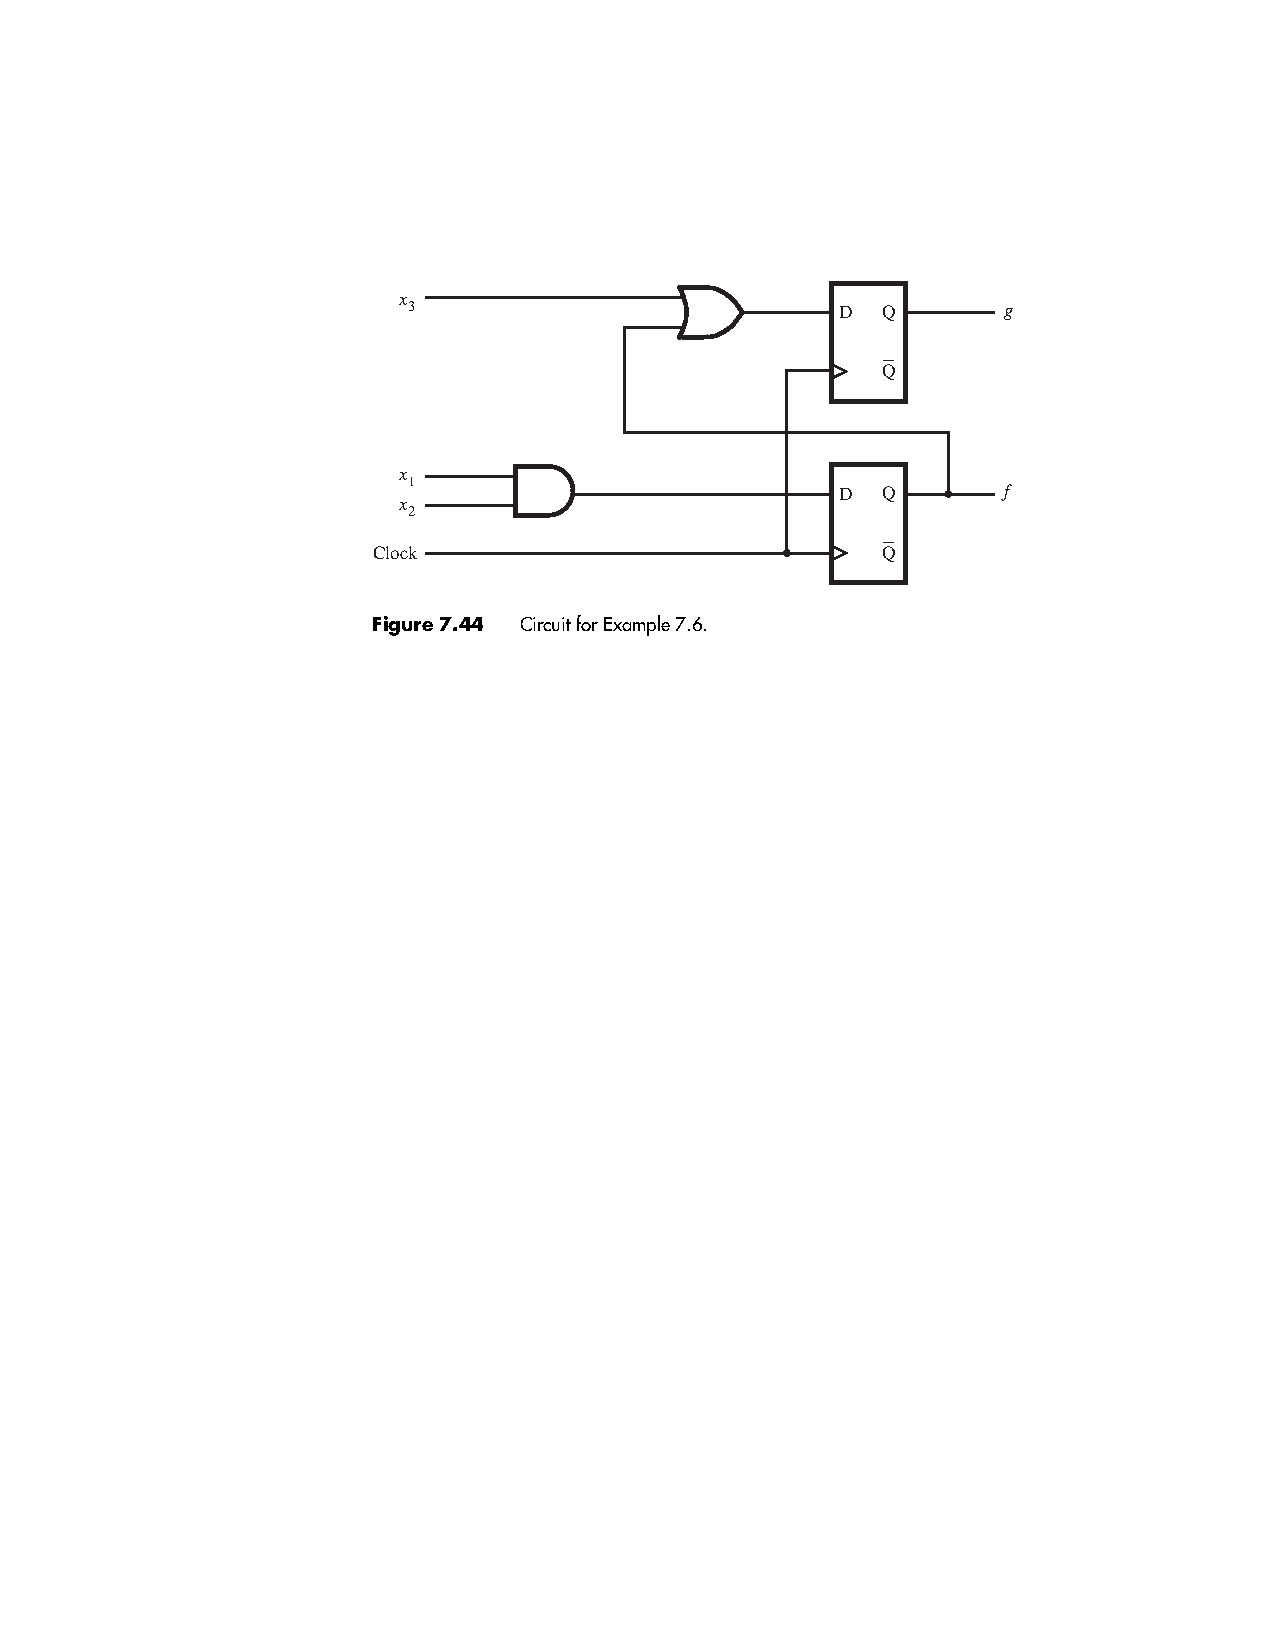
\includegraphics[scale=.6]{figs/VerilogFig7_44}
\end{frame}

\frame{
    \frametitle{Clear e Preset}
    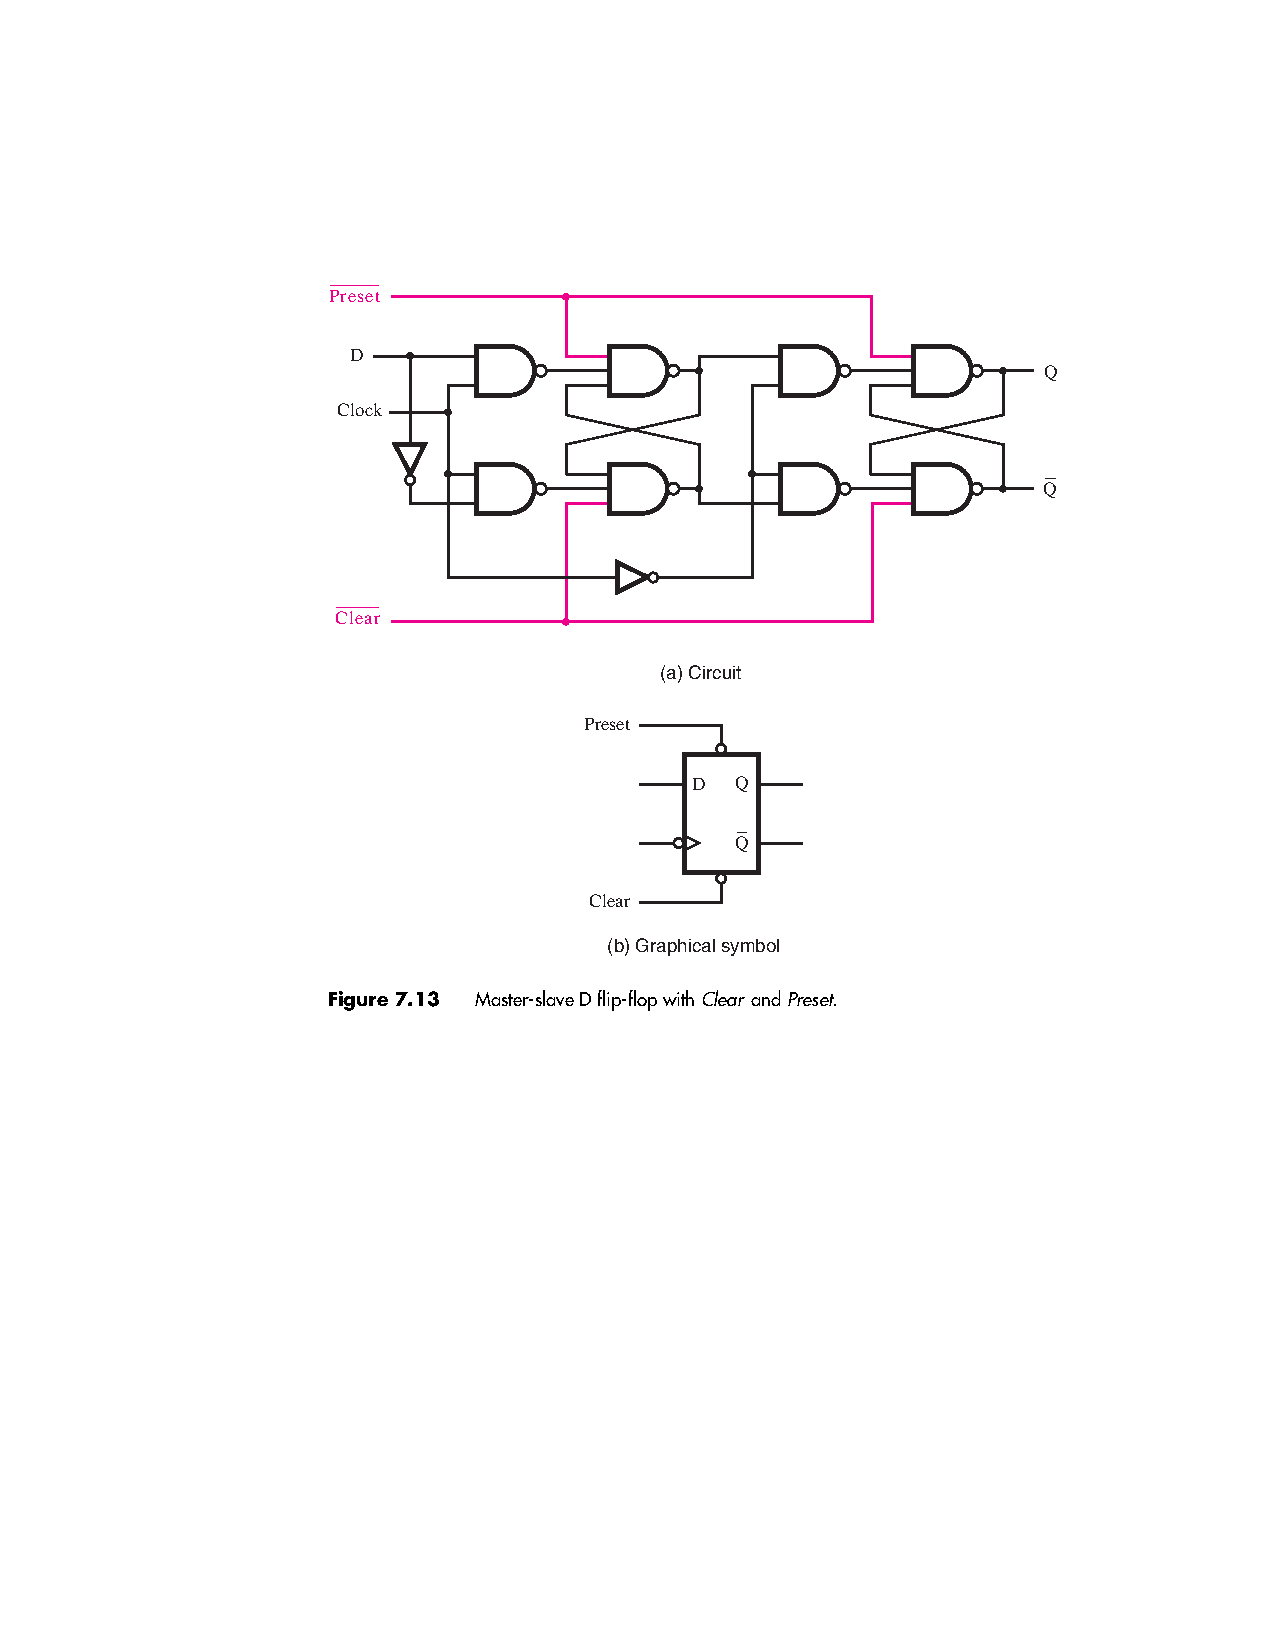
\includegraphics[scale=.7]{figs/VerilogFig7_13}
}

\frame{
    \frametitle{Clear e Preset}
    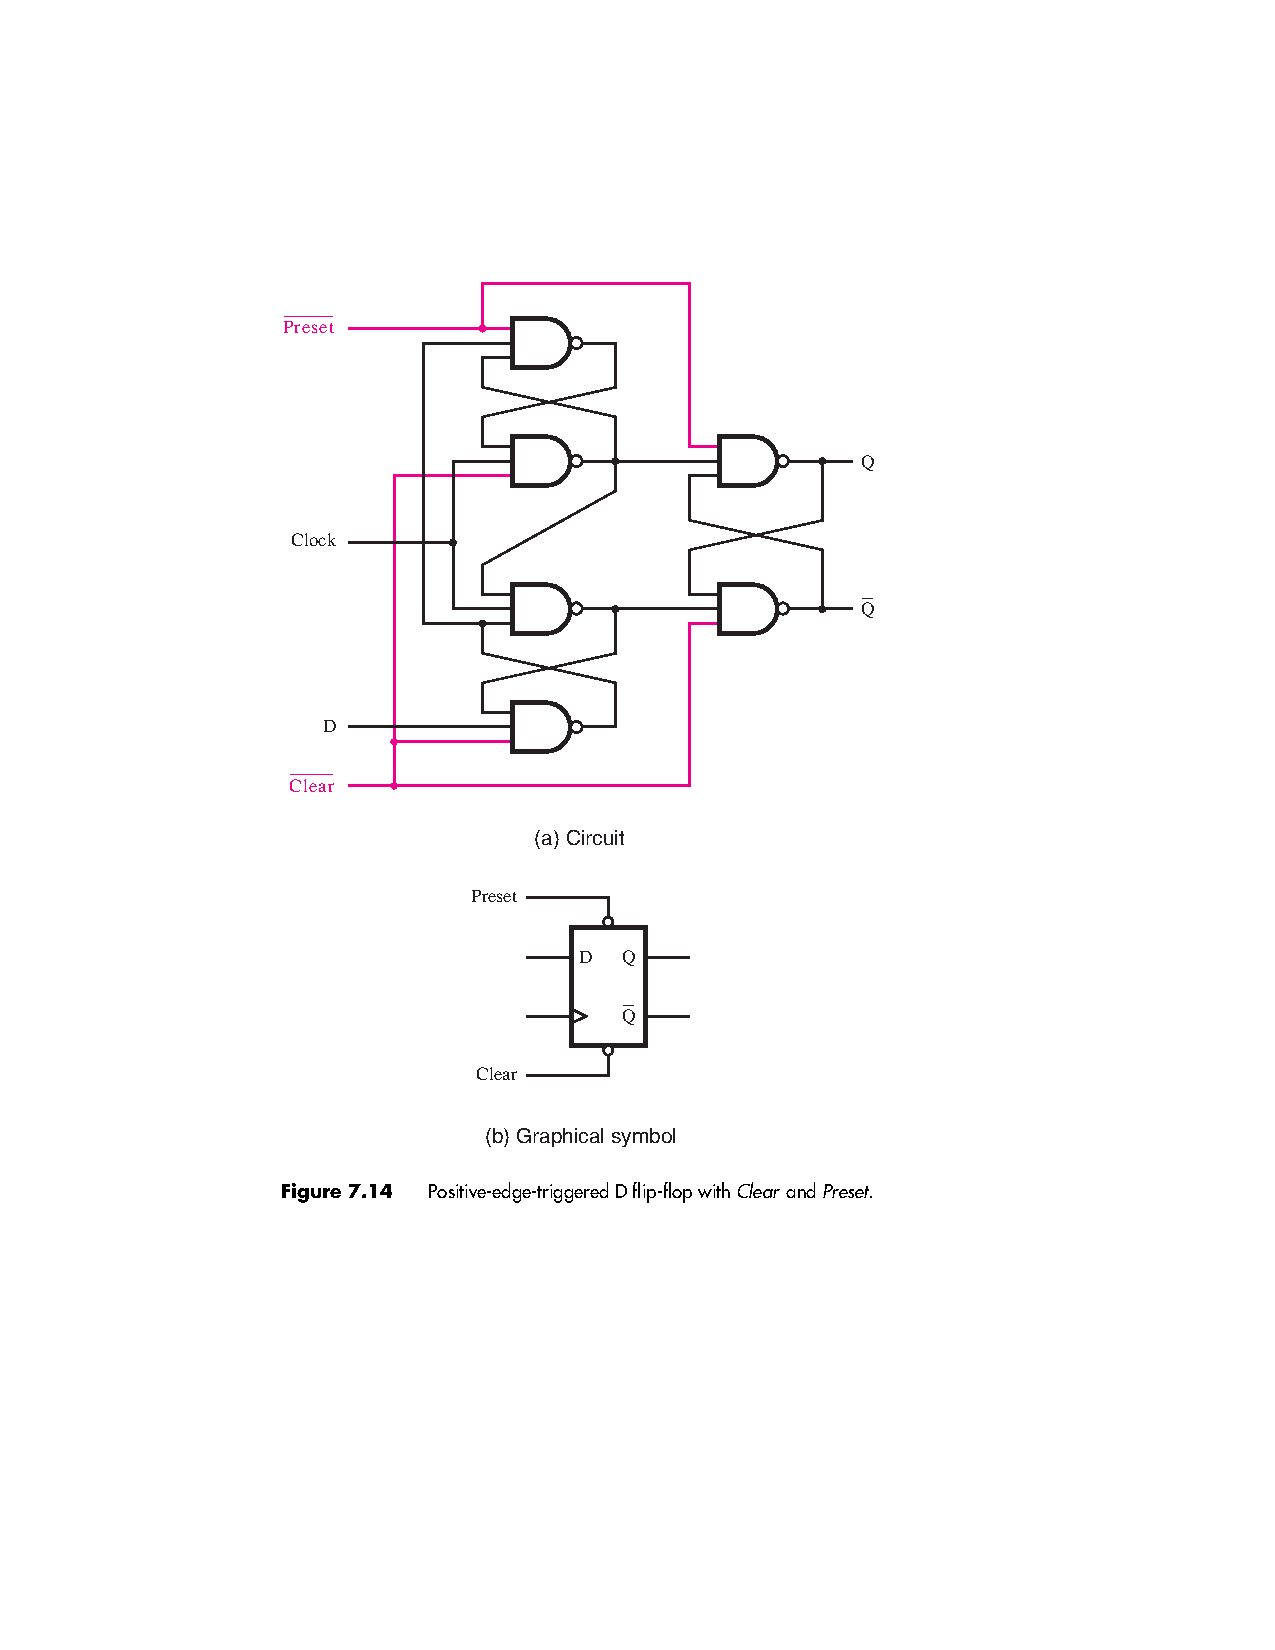
\includegraphics[scale=.55]{figs/VerilogFig7_14}
}

\begin{frame}[fragile]
	\frametitle{Reset Assíncrono (Clear)}
	\begin{verilogcode}
module flipflop(D, Clock, Resetn, Q); 
  input D, Clock, Resetn;
  output Q;
  reg Q;

  always @(negedge Resetn or posedge Clock) 
    if (!Resetn)
      Q <= 0; 
    else
      Q <= D; 
endmodule
	\end{verilogcode}
\end{frame}

\begin{frame}[fragile]
	\frametitle{Reset Síncrono}
	\begin{verilogcode}
module flipflop(D, Clock, Resetn, Q); 
  input D, Clock, Resetn;
  output Q;
  reg Q;

  always @(posedge Clock) 
    if (!Resetn)
      Q <= 0; 
    else
      Q <= D; 
endmodule
	\end{verilogcode}
\end{frame}

\frame{
    \frametitle{Flip-Flop T}
    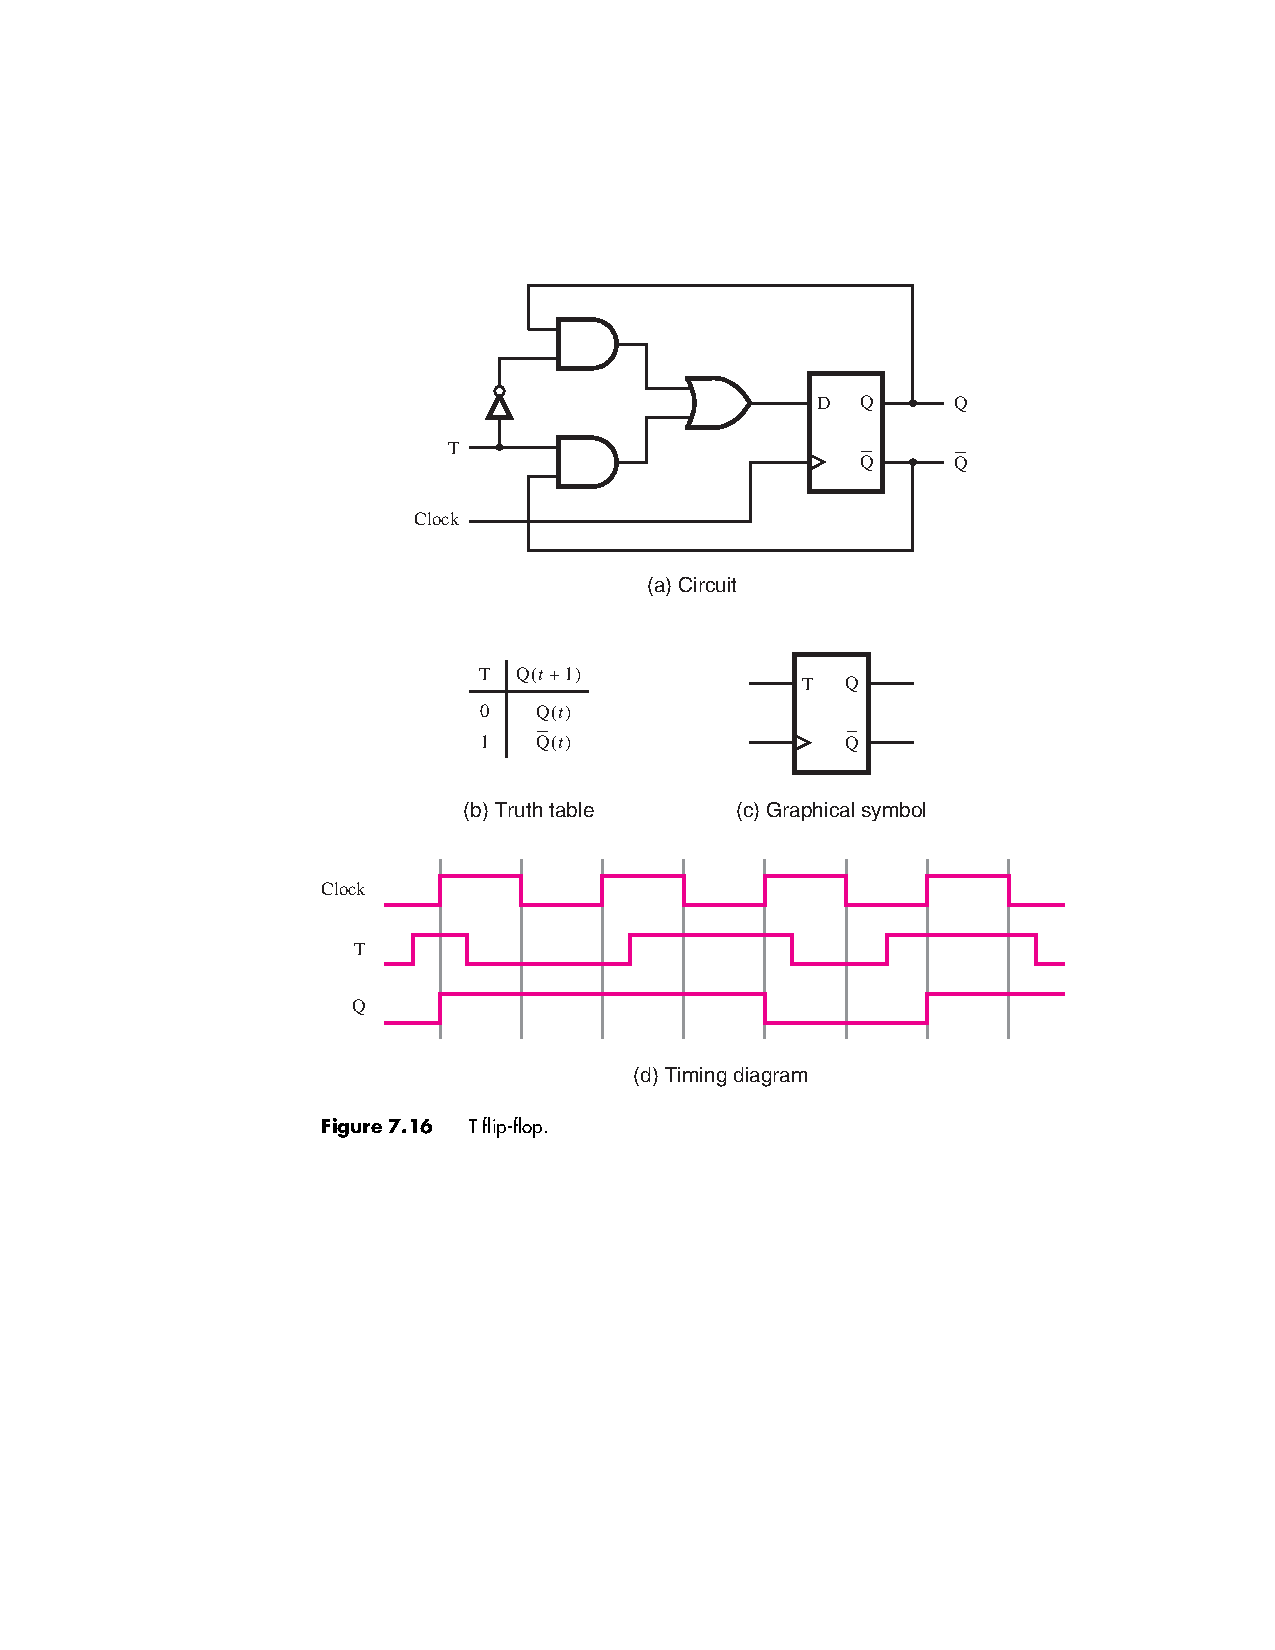
\includegraphics[scale=.6]{figs/VerilogFig7_16}
}

\frame{
    \frametitle{Flip-Flop JK}
    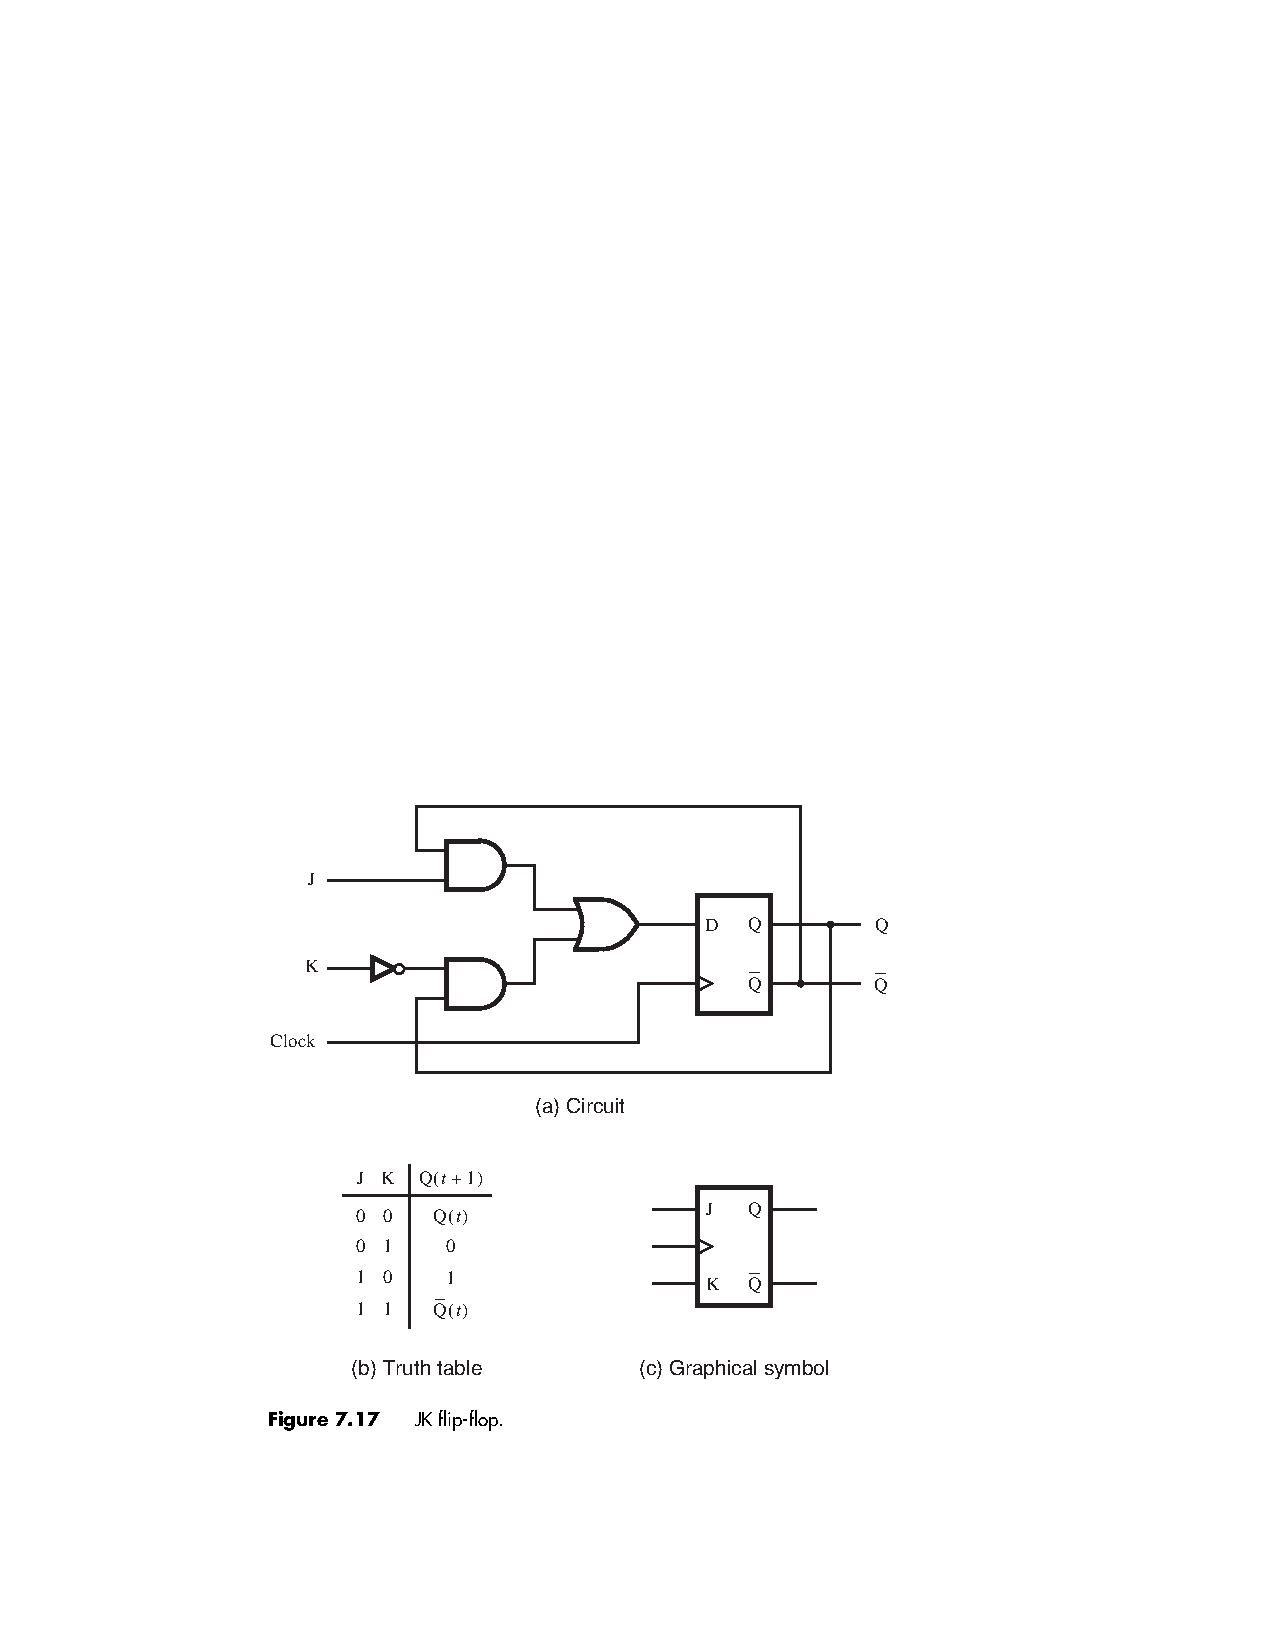
\includegraphics[scale=.6]{figs/VerilogFig7_17}
}

\subsection{Registradores}

\begin{frame}[fragile]
	\frametitle{Registrador de N bits}
	\begin{verilogcode}
module regn (D, Clock, Resetn, Q); 
  parameter n = 16;
  input [n-1:0] D;
  input Clock, Resetn;
  output [n-1:0] Q; 
  reg[n-1:0] Q;

  always @(negedge Resetn or posedge Clock) 
    if (!Resetn)
      Q <= 0; 
    else
      Q <= D; 
endmodule
	\end{verilogcode}
\end{frame}

\frame{
    \frametitle{Registrador de deslocamento}
    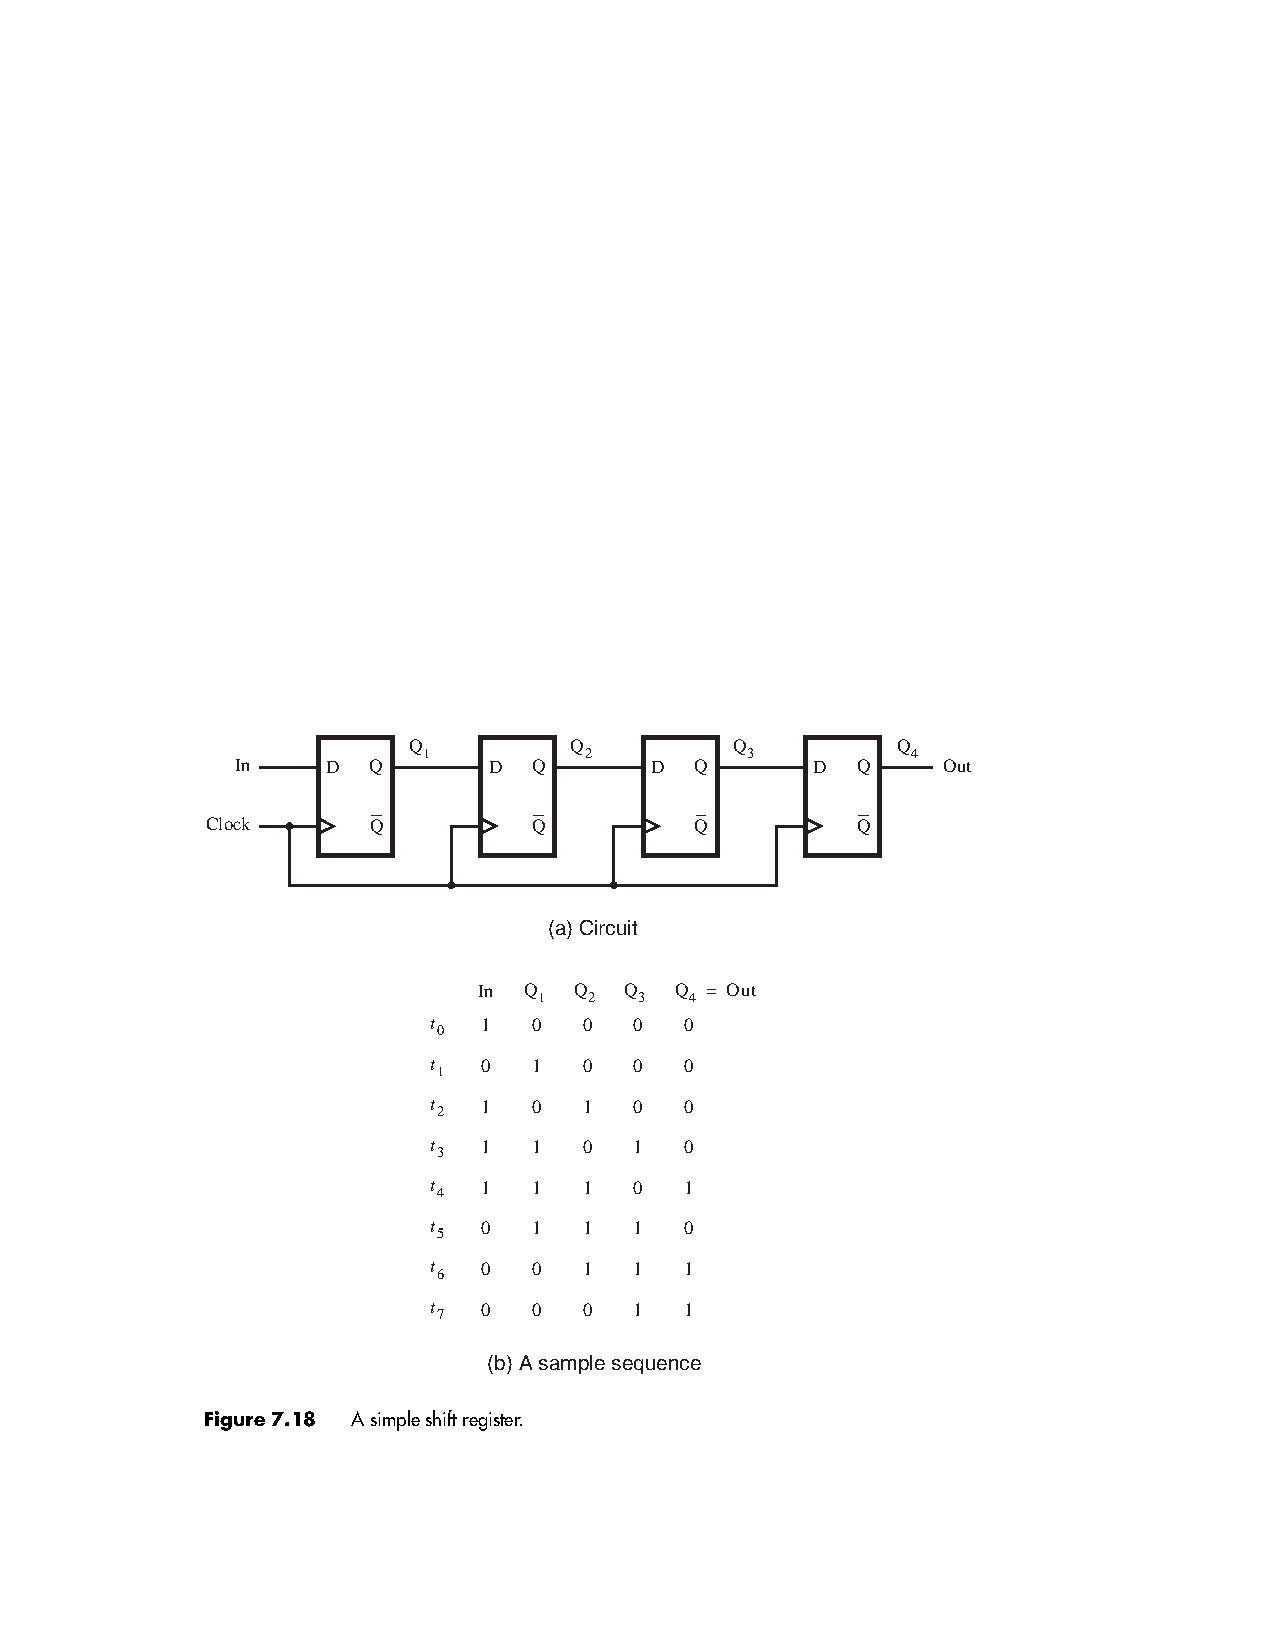
\includegraphics[scale=.7]{figs/VerilogFig7_18}
}

\frame{
    \frametitle{Registrador de deslocamento com acesso paralelo}
    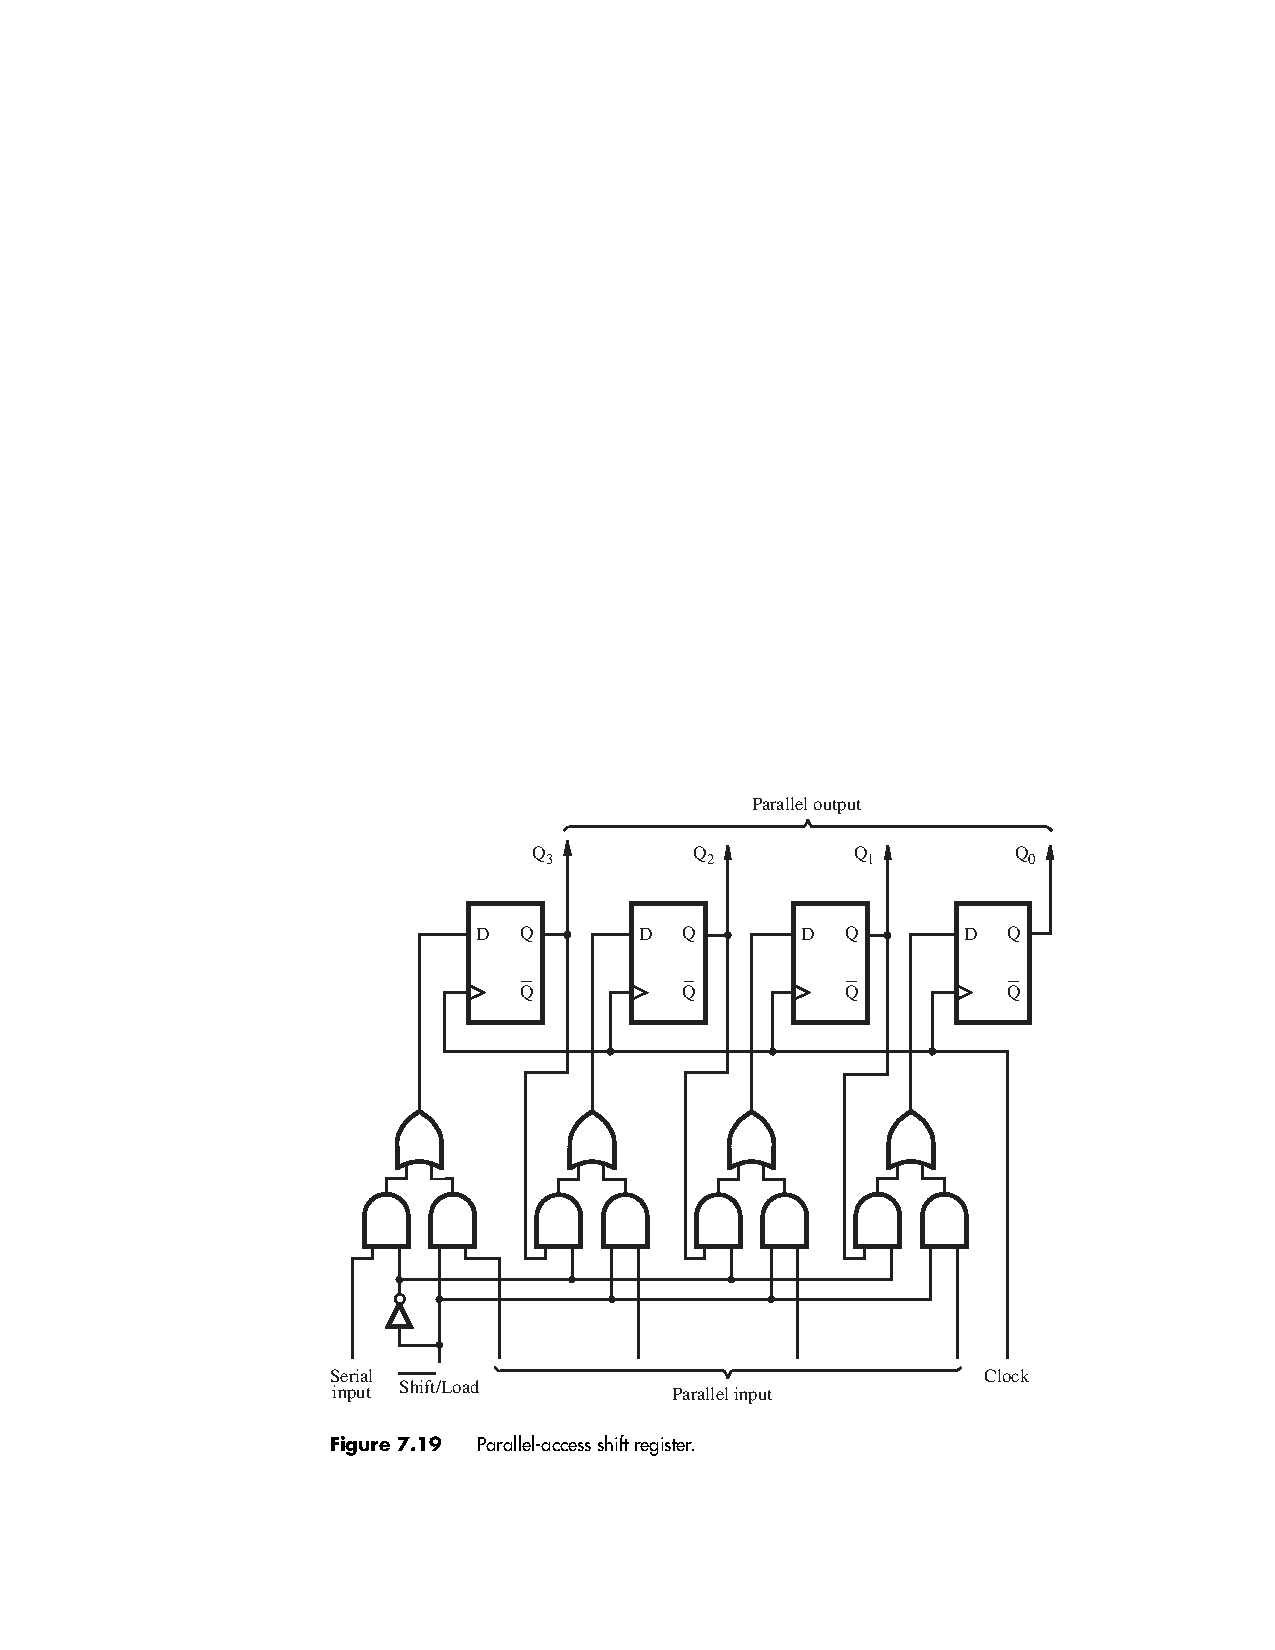
\includegraphics[scale=.7]{figs/VerilogFig7_19}
}

\begin{frame}[fragile]
	\frametitle{Registrador de deslocamento com acesso paralelo}
	\begin{verilogcode}
module muxdff (D0, D1, Sel, Clock, Q); 
  input D0, D1, Sel, Clock;
  output Q;
  reg Q;

  always @(posedge Clock) 
    if (!Sel)
      Q <= D0; 
    else
      Q <= D1; 
endmodule

module shift4 (R, L, w, Clock, Q); 
  input [3:0] R;
  input L, w, Clock;
  output [3:0] Q;
  wire [3:0] Q;
  
  muxdff Stage3 (w,    R[3], L, Clock, Q[3]); 
  muxdff Stage2 (Q[3], R[2], L, Clock, Q[2]); 
  muxdff Stage1 (Q[2], R[1], L, Clock, Q[1]); 
  muxdff Stage0 (Q[1], R[0], L, Clock, Q[0]);
endmodule
	\end{verilogcode}
\end{frame}

\begin{frame}[fragile]
	\frametitle{Implementação alternativa}
	\begin{verilogcode}
module shift4 (R, L, w, Clock, Q); 
  input [3:0] R;
  input L, w, Clock;
  output [3:0] Q;
  reg [3:0] Q;

  always @(posedge Clock) 
    if (L)
      Q <= R; 
    else
    begin
      Q[0] <= Q[1]; 
      Q[1] <= Q[2]; 
      Q[2] <= Q[3]; 
      Q[3] <= w;
    end 
endmodule
	\end{verilogcode}
\end{frame}


\begin{frame}[fragile]
	\frametitle{Implementação genérica}
	\begin{verilogcode}
module shiftn (R, L, w, Clock, Q); 
  parameter n = 16;
  input [n-1:0] R;
  input L, w, Clock;
  output [n-1:0] Q; 
  reg [n-1:0] Q; 
  integer k;

  always @(posedge Clock) 
    if (L)
      Q <= R; 
    else
    begin
      for(k=0; k<n-1; k=k+1)
        Q[k] <= Q[k+1]; 
      Q[n-1] <= w;
    end 
endmodule
	\end{verilogcode}
\end{frame}

\subsection{Contadores}

\frame{
    \frametitle{Contador}
    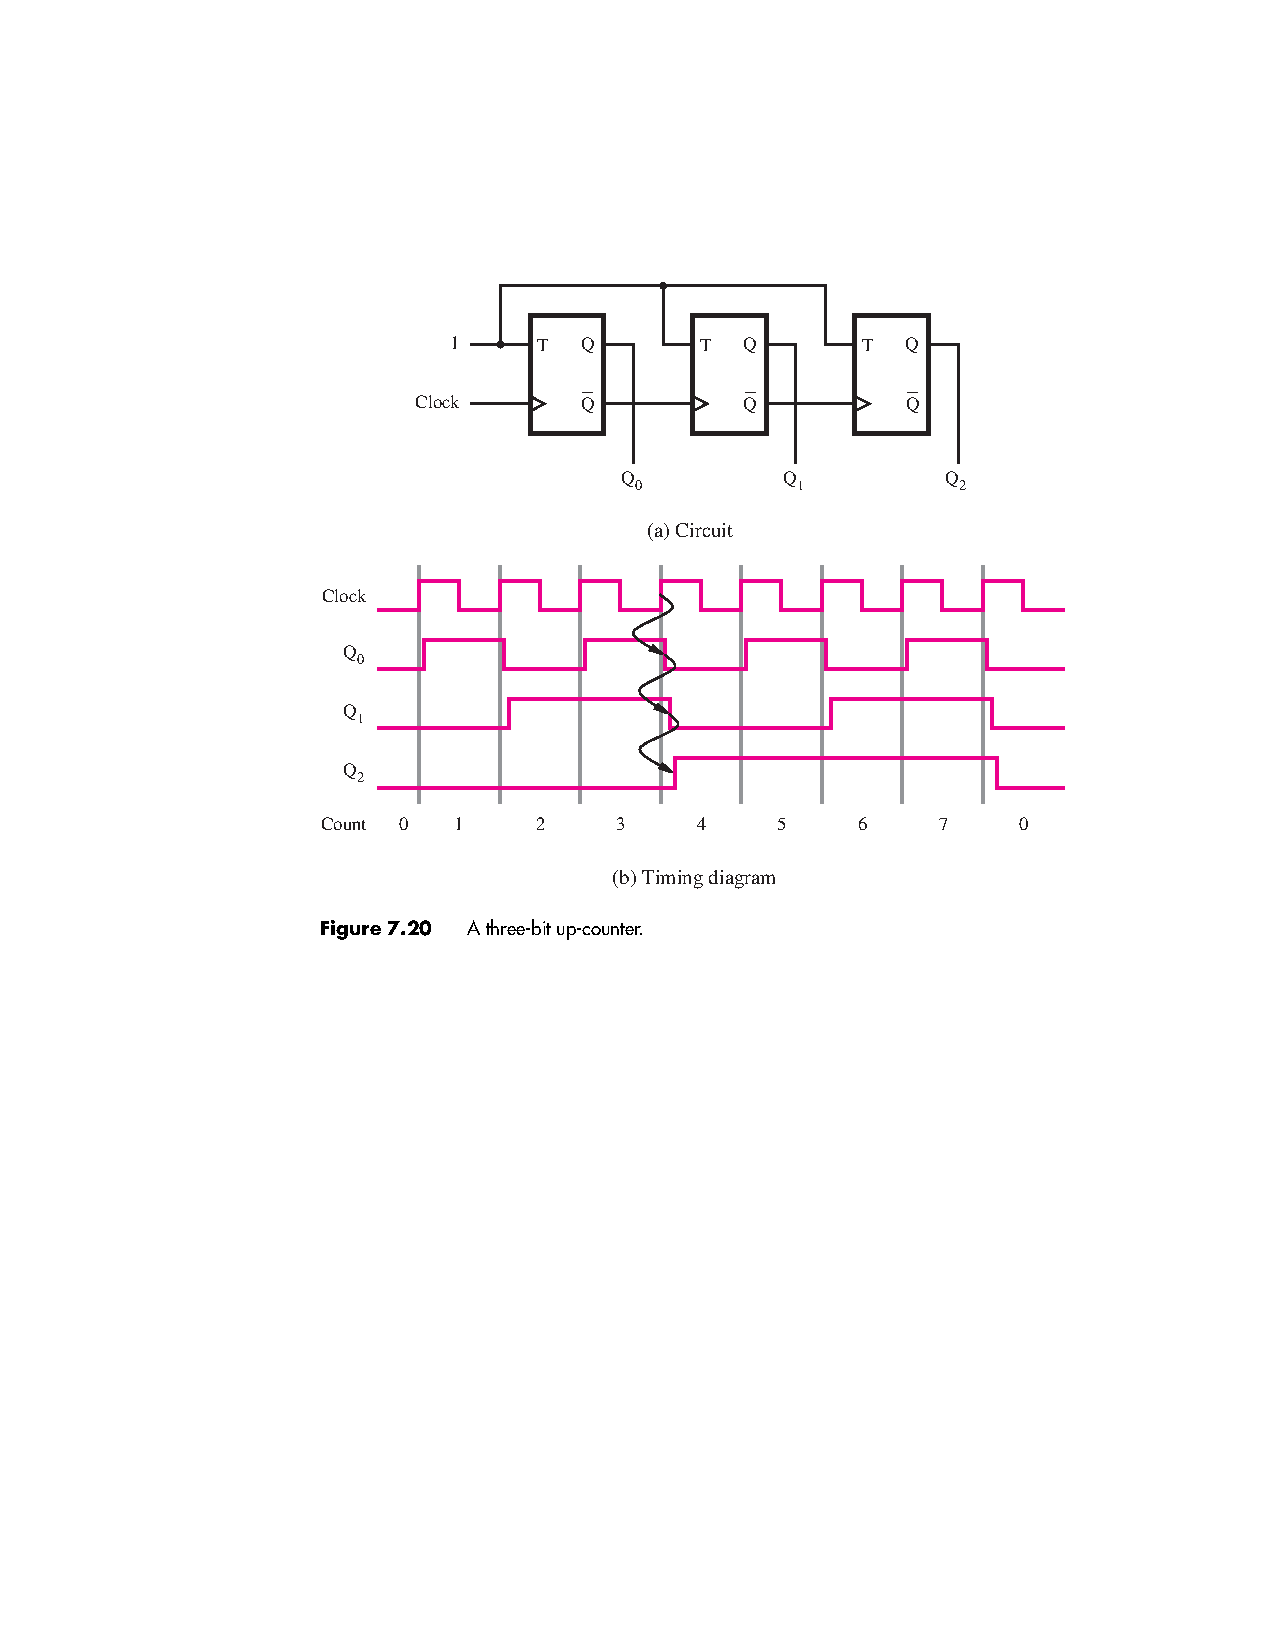
\includegraphics[scale=.7]{figs/VerilogFig7_20}
}

\frame{
    \frametitle{Contador}
    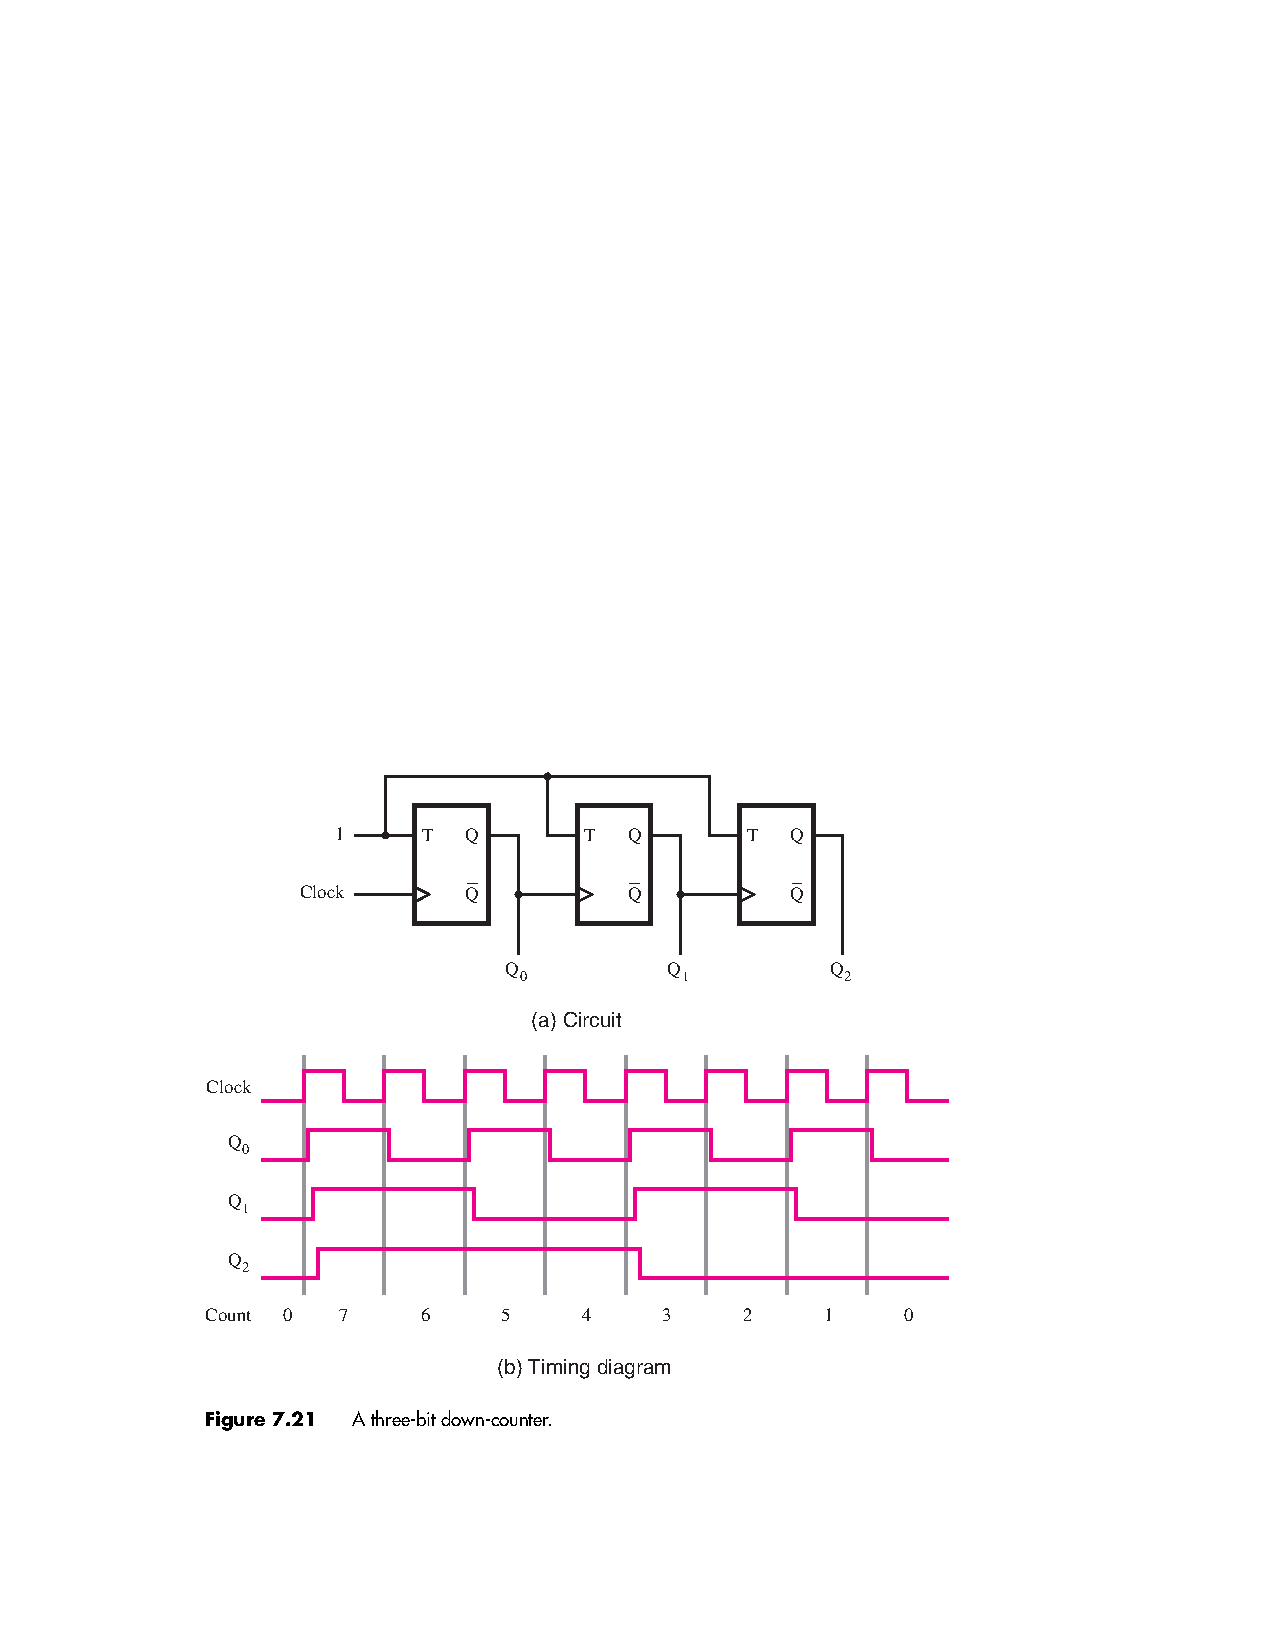
\includegraphics[scale=.7]{figs/VerilogFig7_21}
}

\frame{
    \frametitle{Contador Síncrono}
    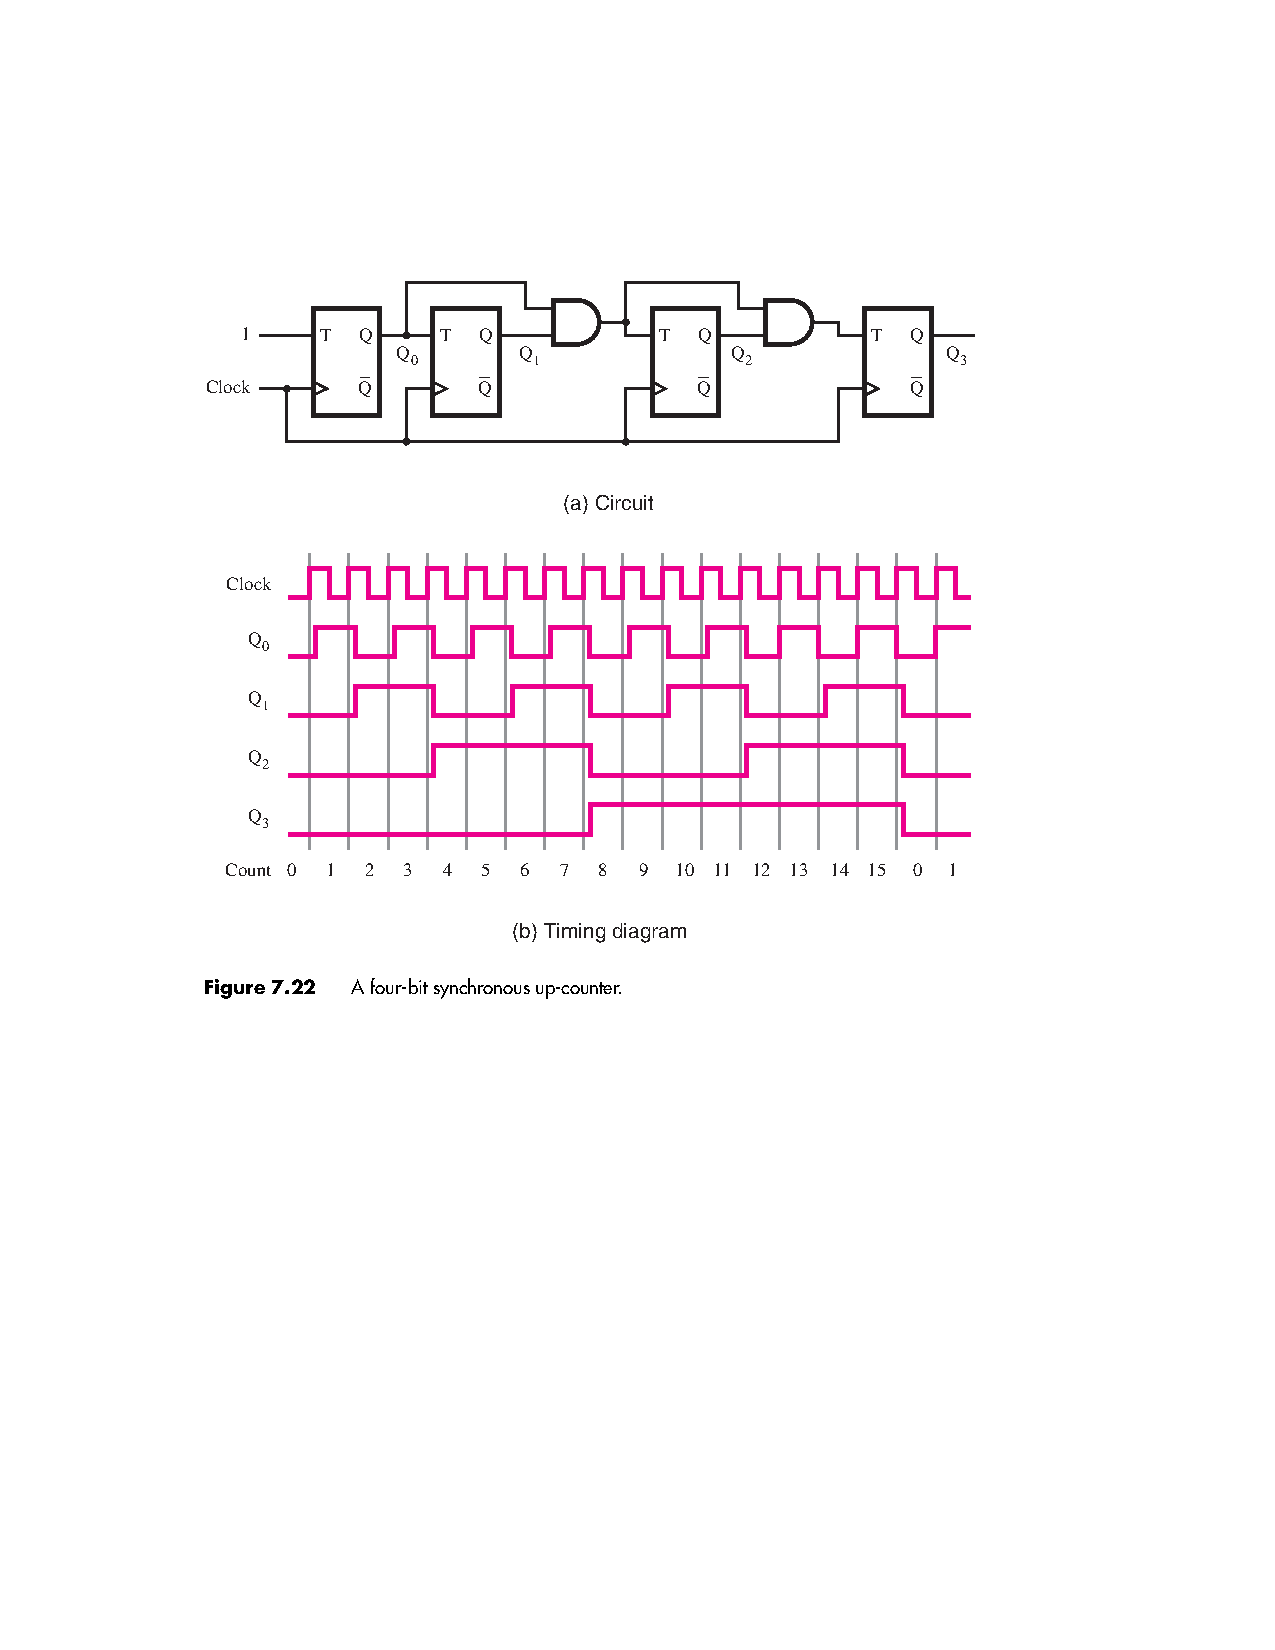
\includegraphics[scale=.7]{figs/VerilogFig7_22}
}

\frame{
    \frametitle{Contador com Enable e Clear}
    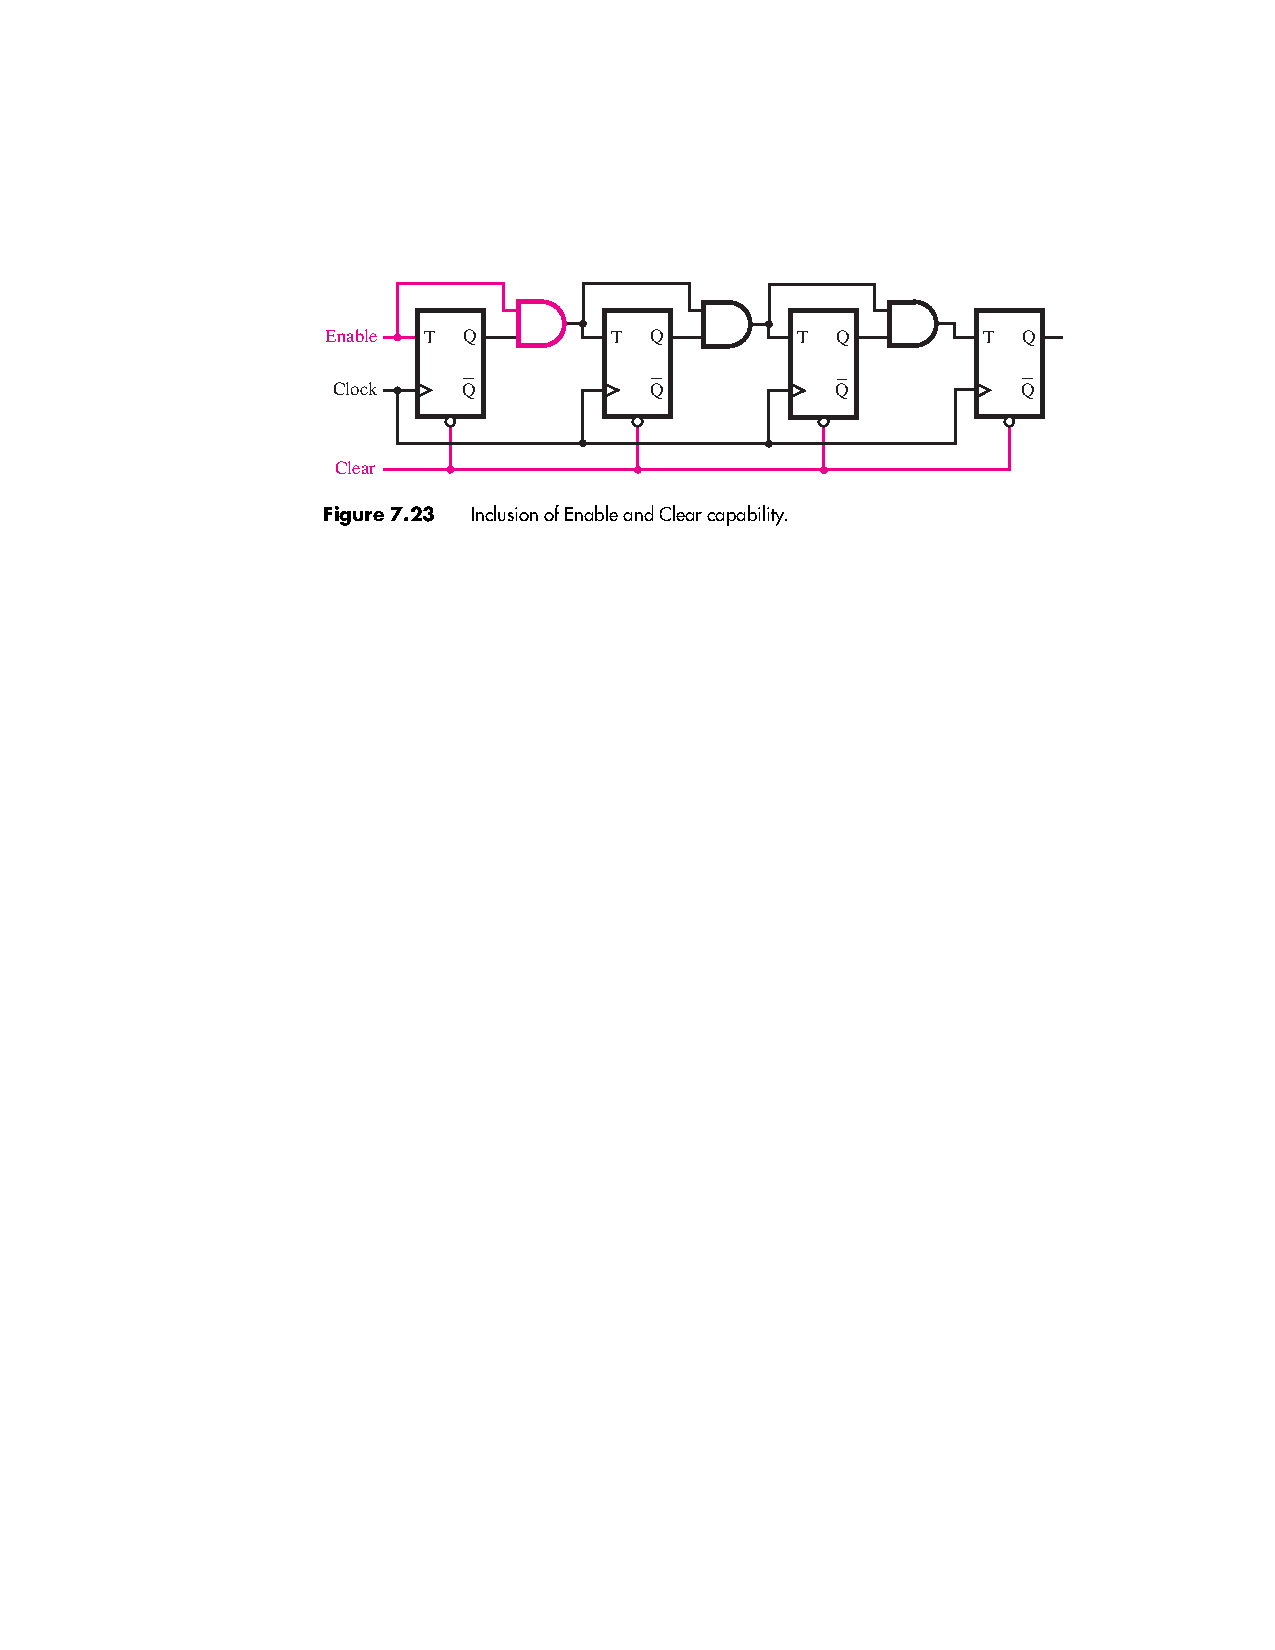
\includegraphics[scale=.7]{figs/VerilogFig7_23}
}

\begin{frame}[fragile]
	\frametitle{Contador com Enable e Reset Assíncrono (Clear)}
	\begin{verilogcode}
module upcount (Resetn, Clock, E, Q); 
  input Resetn, Clock, E;
  output [3:0] Q;
  reg [3:0] Q;

  always @(negedge Resetn or posedge Clock) 
    if (!Resetn)
      Q <= 0; 
    else if (E)
      Q <= Q + 1; 
endmodule
	\end{verilogcode}
\end{frame}

\begin{frame}[fragile]
	\frametitle{Contador com Carga}
	\begin{verilogcode}
module upcount (R, Resetn, Clock, E, L, Q); 
  input [3:0] R;
  input Resetn, Clock, E, L;
  output [3:0] Q;
  reg [3:0] Q;

  always @(negedge Resetn or posedge Clock) 
    if (!Resetn)
      Q <= 0; 
    else if (L)
      Q <= R; 
    else if (E)
      Q <= Q + 1; 
endmodule
	\end{verilogcode}
\end{frame}

\begin{frame}[fragile]
	\frametitle{Contador up/down}
	\begin{verilogcode}
module updowncount (R, Clock, L, E, up_down, Q); 
  parameter n = 8;
  input [n-1:0] R;
  input Clock, L, E, up down;
  output [n-1:0] Q; 
  reg[n 1:0]Q; 
  integer direction;
  
  always @(posedge Clock) 
  begin
    if (up_down) 
      direction = 1;
    else
      direction = -1; 
    if (L)
      Q <= R; 
    else if (E)
      Q <= Q + direction; 
  end
endmodule
	\end{verilogcode}
\end{frame}

\subsection{Implementação (III)}

\begin{frame}[fragile]
	\frametitle{Perigo!: Especificação Incompleta}
	\begin{columns}
        \column{0.4\textwidth}
        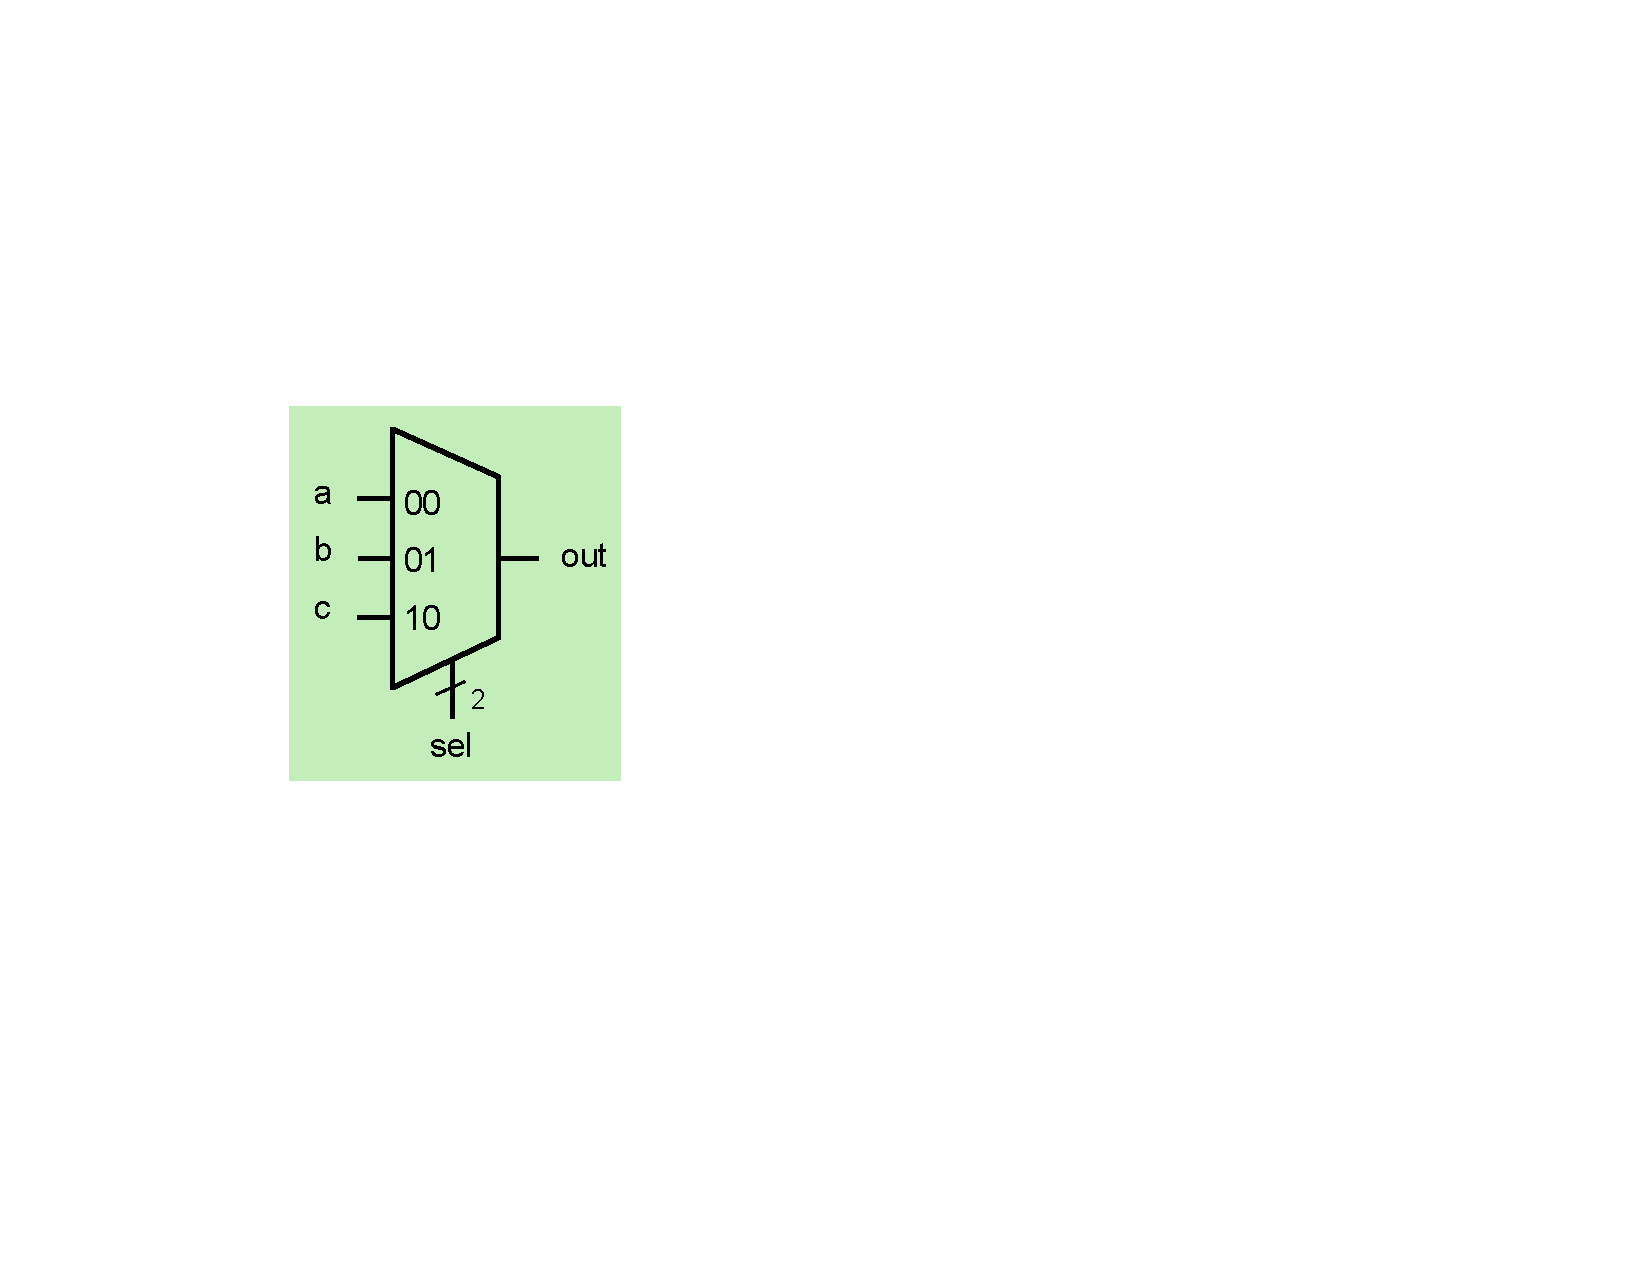
\includegraphics[scale=.5]{figs/Mux3to1}
        \column{0.6\textwidth}
	    \begin{verilogcode}
module mux3to1(a, b, c, sel, out);
  input [1:0] sel;
  input a, b, c;
  output out;
  reg out;
  
  always @(a or b or c or sel)
  begin
    case (sel)
      2'b00: out = a;
      2'b01: out = b;
      2'b10: out = c;
    endcase
  end
endmodule
        \end{verilogcode}
    \end{columns}
\end{frame}

\begin{frame}[fragile]
	\frametitle{Perigo!: Especificação Incompleta}
    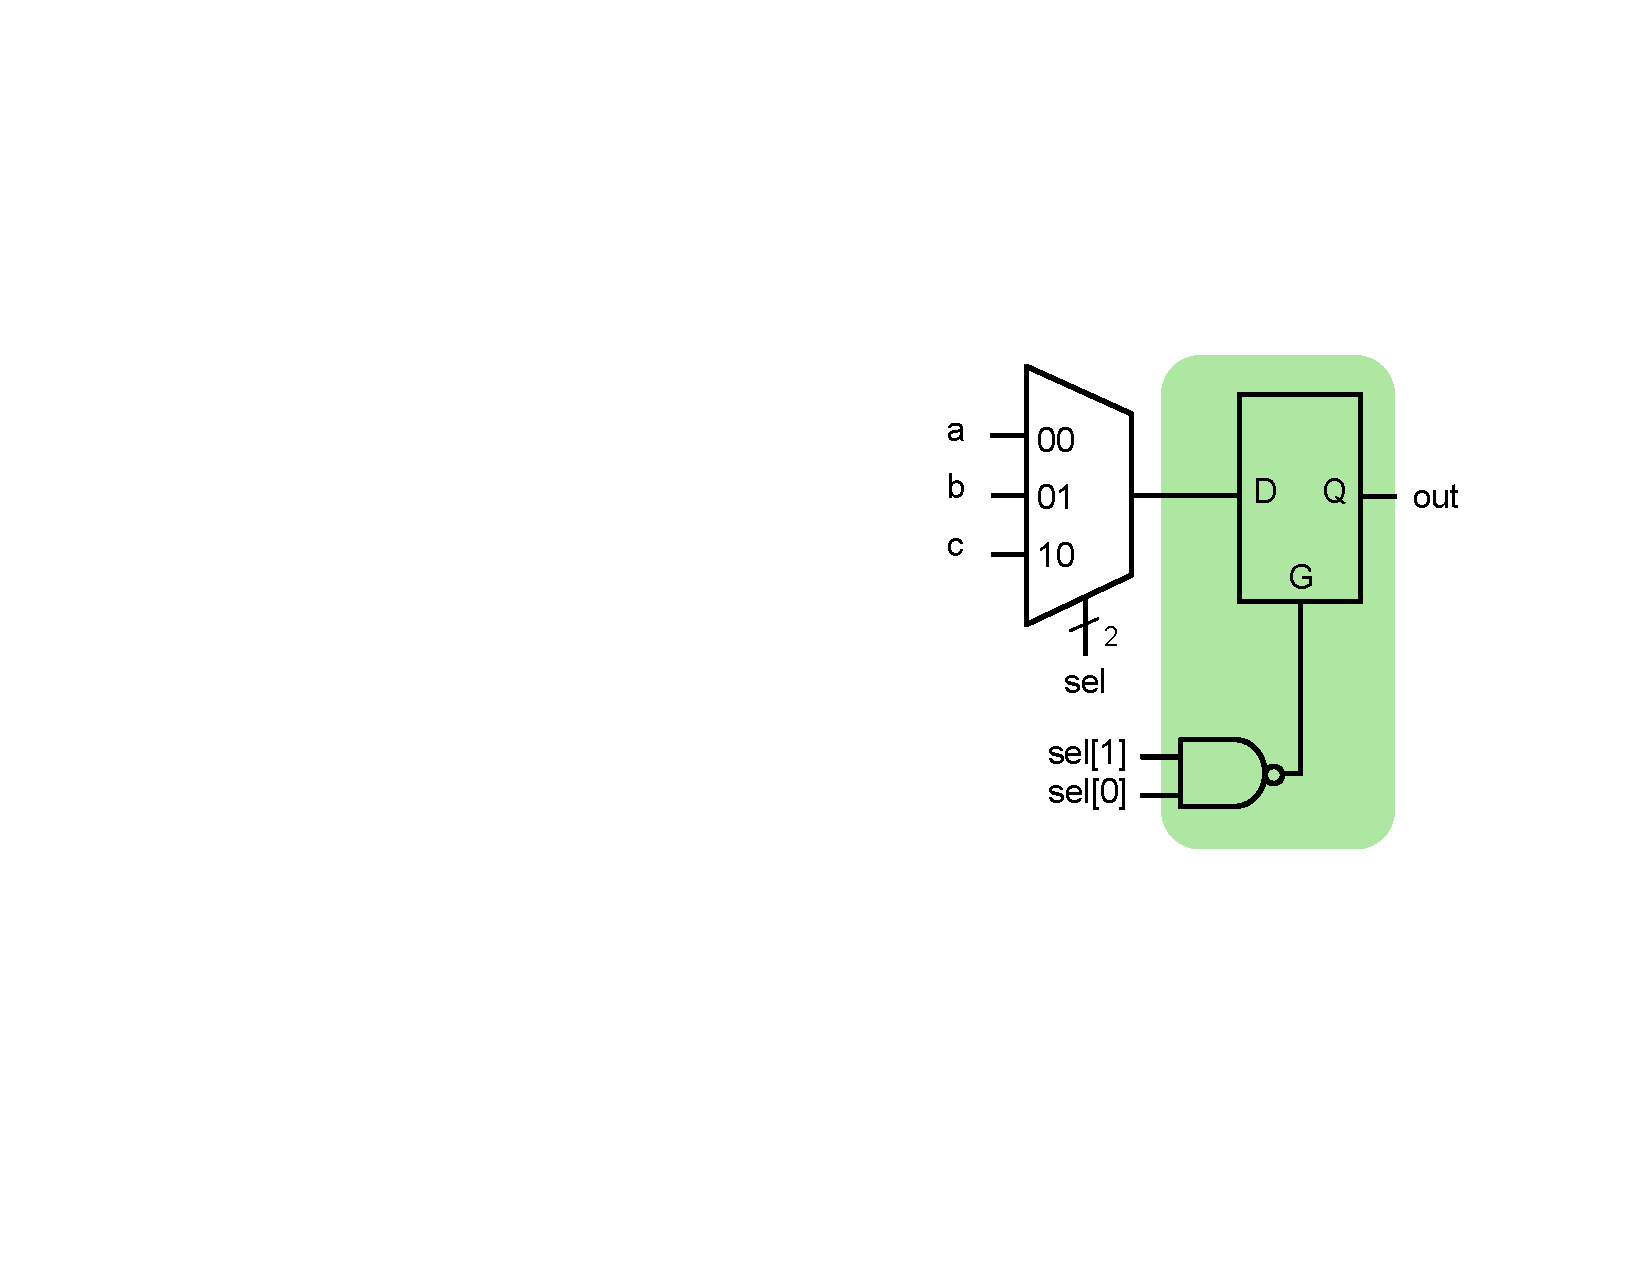
\includegraphics[scale=.5]{figs/Mux3to1Latch}
\end{frame}

\begin{frame}[fragile]
	\frametitle{Evitando a Especificação Incompleta}
	\begin{verilogcode}
  always @(a or b or c or sel)
  begin
    out = 1'bx
    case (sel)
      2'b00: out = a;
      2'b01: out = b;
      2'b10: out = c;
    endcase
  end
    \end{verilogcode}
	\begin{verilogcode}
  always @(a or b or c or sel)
  begin
    case (sel)
      2'b00: out = a;
      2'b01: out = b;
      2'b10: out = c;
      default: out = 1'bx
    endcase
  end
    \end{verilogcode}
\end{frame}

\begin{frame}[fragile]
	\frametitle{Perigo!: Prioridade Indesejada}
	\begin{columns}
        \column{0.4\textwidth}
        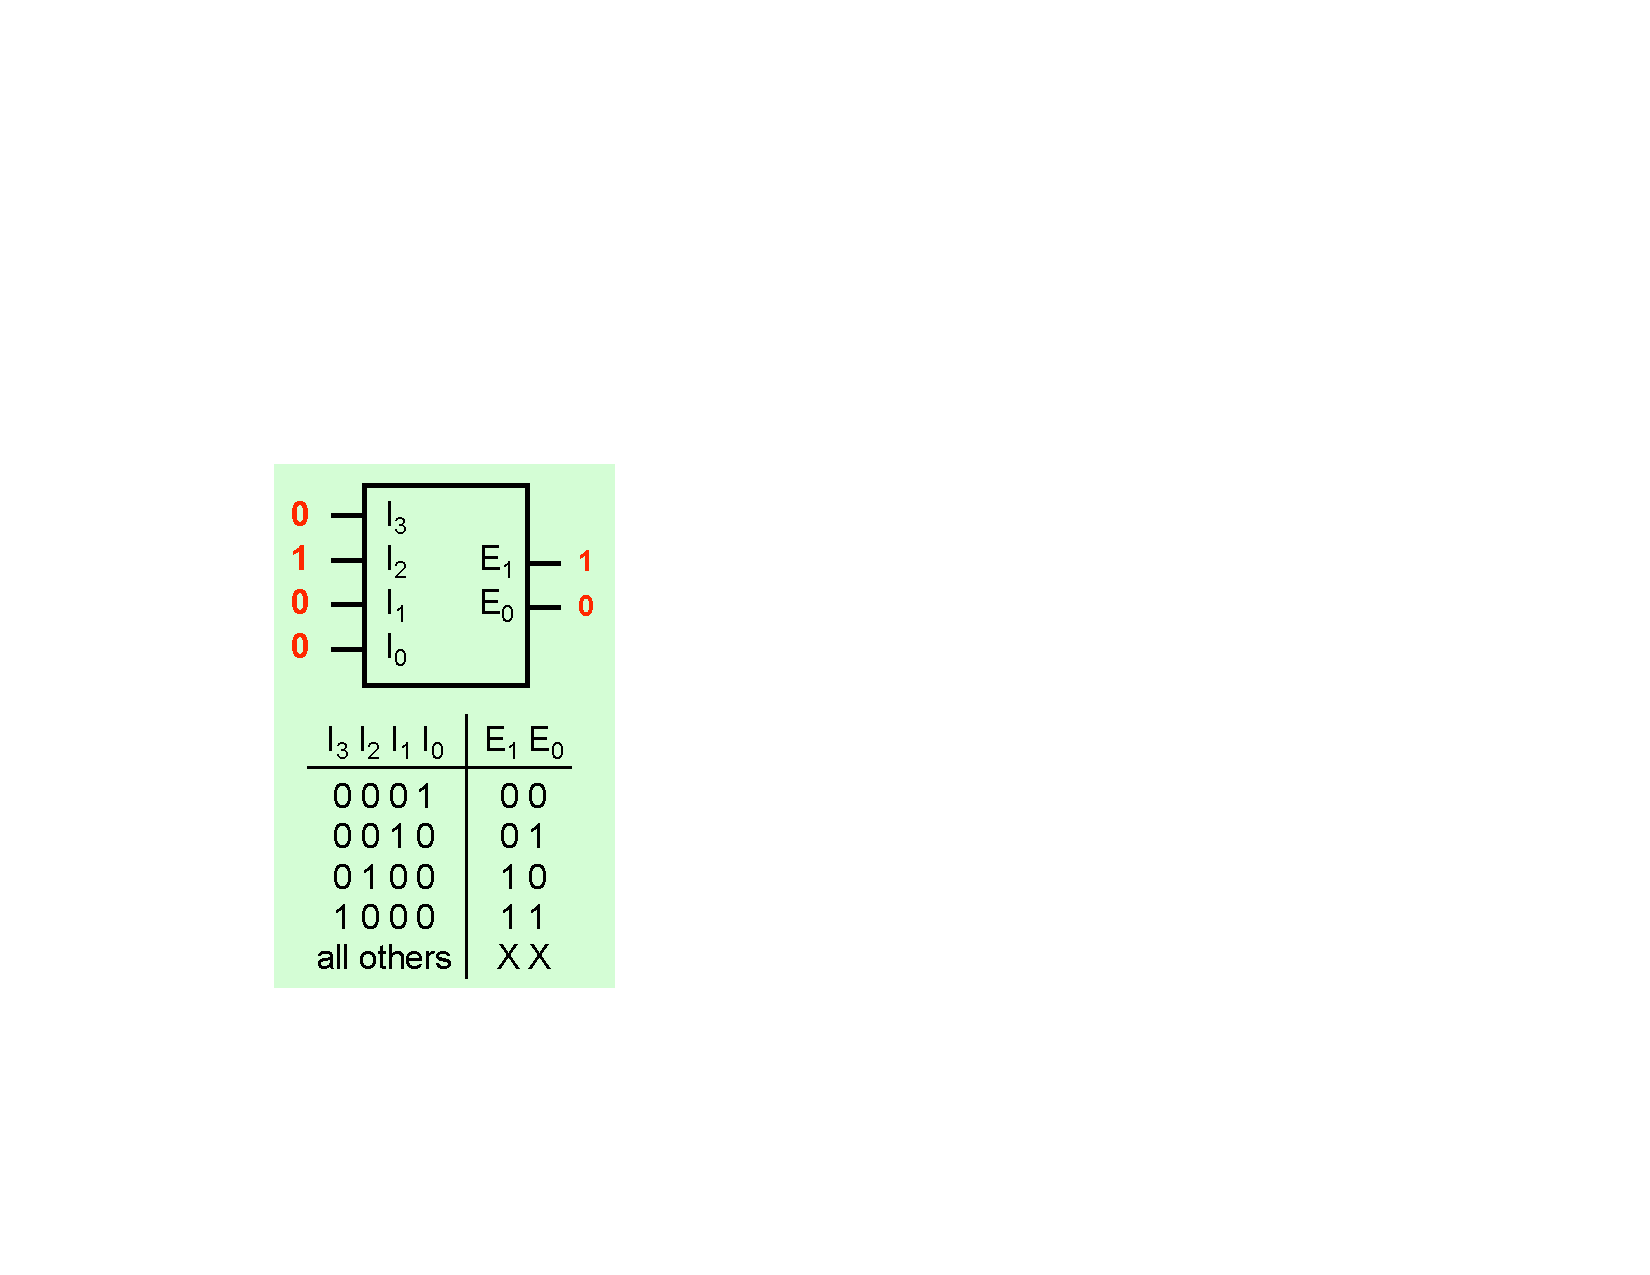
\includegraphics[scale=.5]{figs/Encoder4to2}
        \column{0.6\textwidth}
    	\begin{verilogcode}
module binary_encoder(i, e); 
  input [3:0] i;
  output [1:0] e;
  reg e;
 
  always @(i)
  begin
    if (i[0]) 
      e = 2'b00; 
    else if (i[1]) 
      e = 2'b01; 
    else if (i[2]) 
      e = 2'b10; 
    else if (i[3]) 
      e = 2'b11; 
    else 
      e = 2'bxx;
  end
endmodule
        \end{verilogcode}
    \end{columns}
\end{frame}

\begin{frame}[fragile]
	\frametitle{Perigo!: Prioridade Indesejada}
    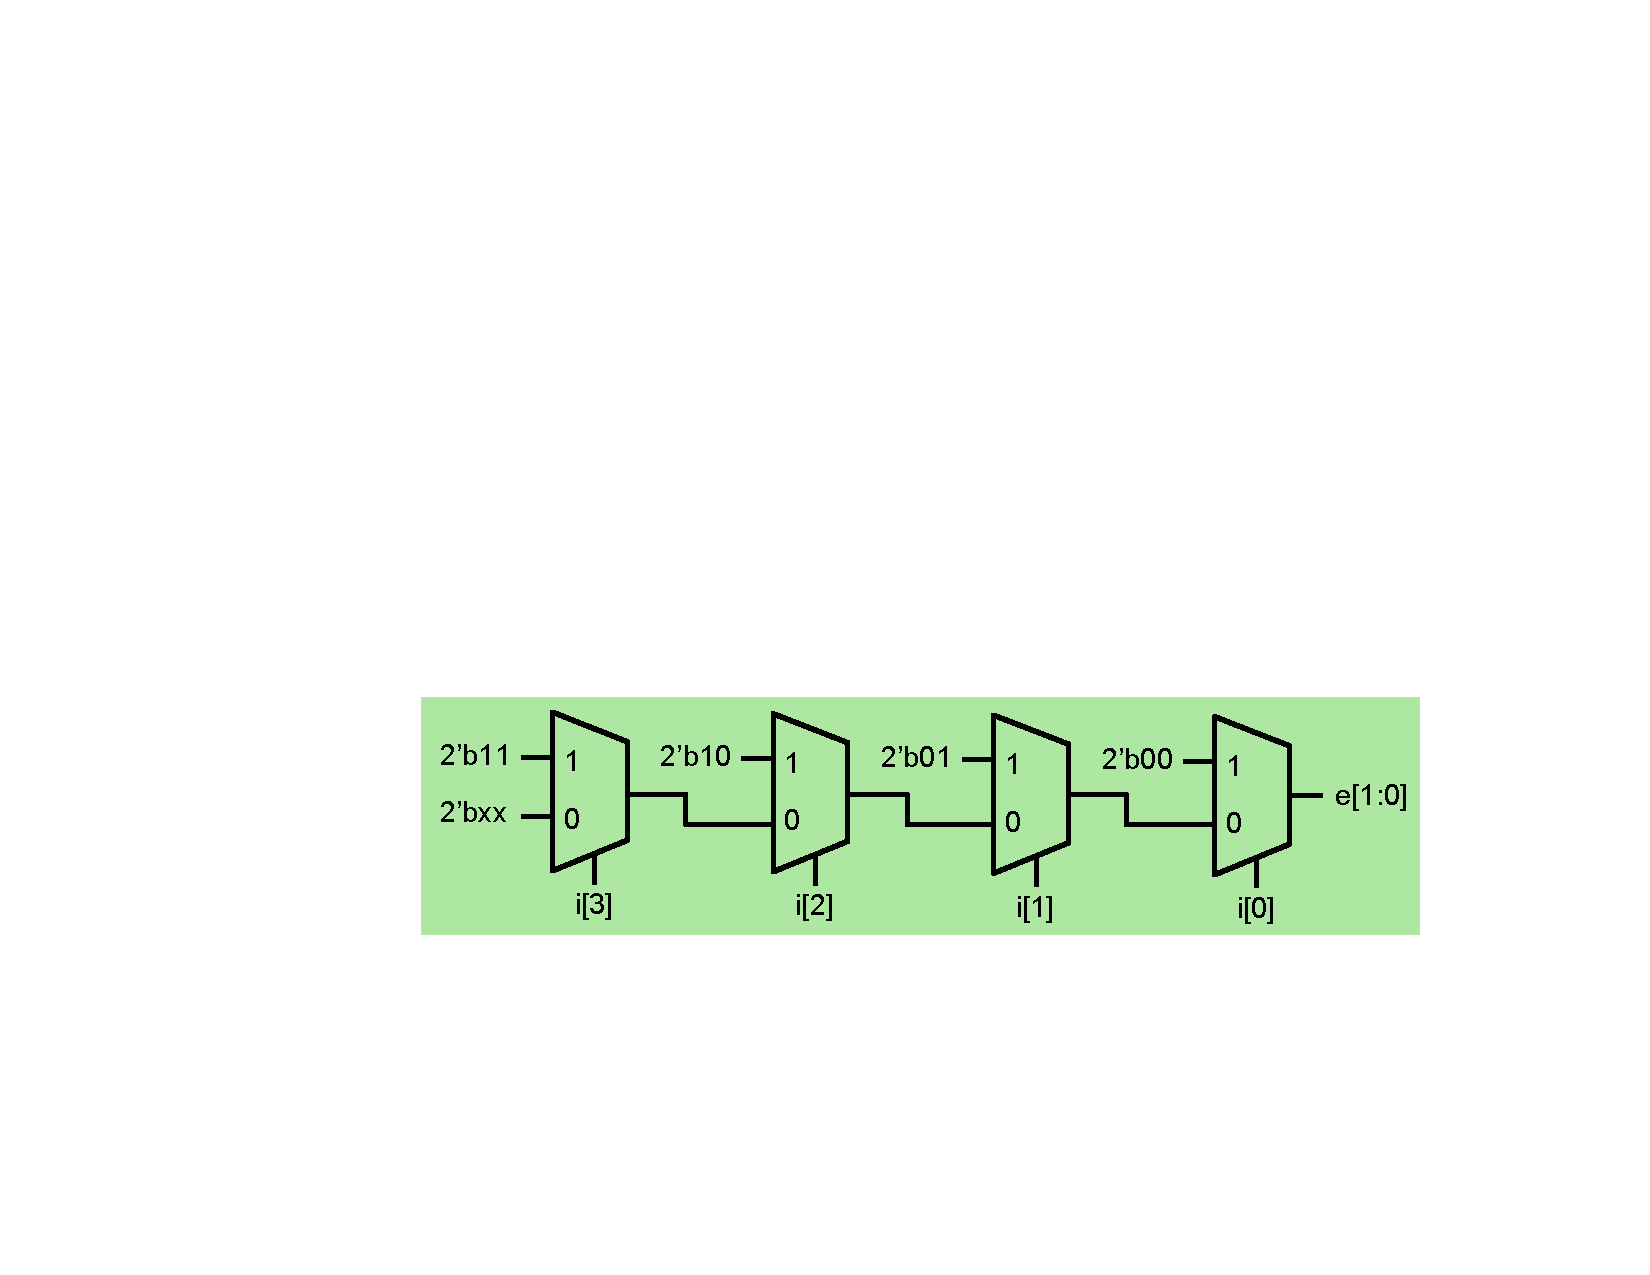
\includegraphics[scale=.5]{figs/Encoder4to2Pri}
\end{frame}

\begin{frame}[fragile]
	\frametitle{Evitando Prioridade Indesejada}
	\begin{columns}
        \column{0.4\textwidth}
        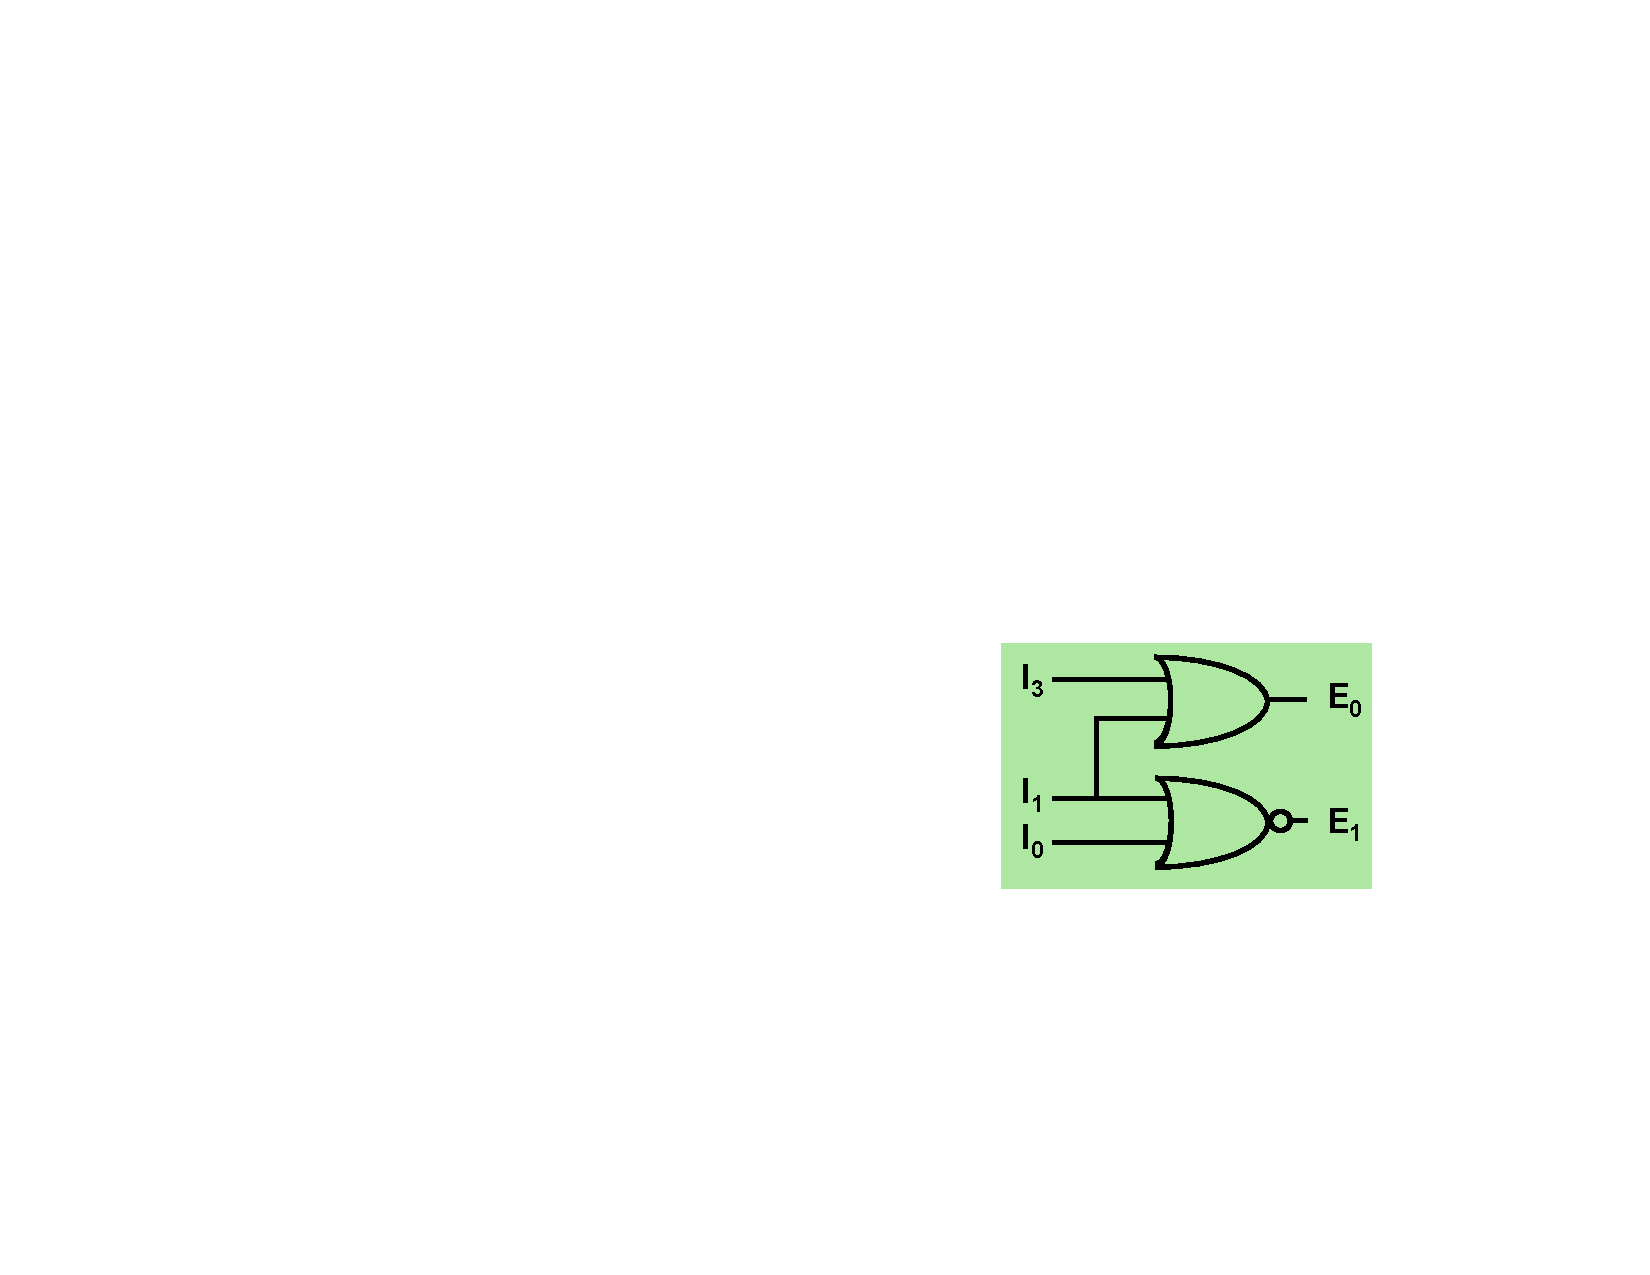
\includegraphics[scale=.5]{figs/Encoder4to2Min}
        \column{0.6\textwidth}
    	\begin{verilogcode}
module binary_encoder(i, e); 
  input [3:0] i;
  output [1:0] e;
  reg e;
 
  always @(i)
  begin
    if (i == 4'b0001) 
      e = 2'b00; 
    else if (i == 4'b0010) 
      e = 2'b01; 
    else if (i == 4'b0100) 
      e = 2'b10; 
    else if (i == 4'b1000) 
      e = 2'b11; 
    else 
      e = 2'bxx;
  end
endmodule
        \end{verilogcode}
    \end{columns}
\end{frame}

\section<presentation>{Bibliografia}

\begin{frame}[allowframebreaks]
  \frametitle<presentation>{Bibliografia}
    
  \begin{thebibliography}{10}
    
  \beamertemplatebookbibitems

    \bibitem{Brown2014}
        Stephen Brown, Zvonko Vranesic 
        \newblock {\em \href{http://mhhe.com/engcs/electrical/brownvranesic/}{Fundamentals of Digital Logic with Verilog Design, 3/e}}.
        \newblock McGraw-Hill, 2014.
  
  \beamertemplatearticlebibitems
  
    \bibitem{Altera2015}
        Altera Corp. 
        \newblock {\em \href{https://www.altera.com/content/dam/altera-www/global/en_US/pdfs/literature/hb/qts/qts_qii5v1.pdf}{Quartus II Handbook Volume 1: Design and Synthesis}}
        \newblock Altera Corp., 2015. 
  
%   % Followed by interesting articles. Keep the list short. 

%   \bibitem{Someone2000}
%     S.~Someone.
%     \newblock On this and that.
%     \newblock {\em Journal of This and That}, 2(1):50--100,
%     2000.
  \end{thebibliography}
\end{frame}

\begin{frame}
	\titlepage
\end{frame} 

\end{document}
